% ---- ETD Document Class and Useful Packages ---- %
\documentclass{ucetd}
\usepackage{subfigure,epsfig,amsfonts}
\usepackage{natbib}
\usepackage{amsmath}
\usepackage{amssymb}
\usepackage{amsthm}
% Add extra packages I need
% Packages used by pandoc when converting Markdown to LaTeX
\usepackage{fixltx2e}
\usepackage{longtable}
\usepackage{booktabs}
% Make cross-references hyperlinks (also format URLs with \url).
% Specify breaklinks so that titles in table of contents linewrap.
\usepackage[breaklinks]{hyperref}
% Fix to use hyperref with UCETD template (from Jason Torres)
\renewcommand{\etdChapterHeadFormat}[1]{\uppercase{#1}}
% Ability to split long captions across pages
\usepackage{ccaption}
% Crop figures
\usepackage{graphicx}
% Add footnote to List of Tables about the supplementary files
\renewcommand{\listtablename}{List of Tables
  \footnote{Note: Due to the large size of some tables, the tables
  have been provided in a supplementary file accompanying the
  dissertation. In such cases, the page number provided below directs
  the reader to a table's caption.
}}
% Nice tilde
% http://tex.stackexchange.com/questions/9363/how-does-one-insert-a-backslash-or-a-tilde-into-latex/9372#comment47661_9372
\newcommand{\mytilde}{\raise.17ex\hbox{$\scriptstyle\mathtt{‌​\sim}$}}


%% Use these commands to set biographic information for the title page:
\title{Investigating susceptibility to tuberculosis using functional genomics approaches}
\author{John David Blischak}
\department{Genetics}
\division{Biological Sciences}
\degree{Doctor of Philosophy}
\date{December 2016}

%% Use these commands to set a dedication and epigraph text
\dedication{Dedication Text}
\epigraph{Epigraph Text}


\begin{document}
%% Basic setup commands
% If you don't want a title page comment out the next line and uncomment the line after it:
\maketitle
%\omittitle

% These lines can be commented out to disable the copyright/dedication/epigraph pages
\makecopyright
%\makededication
%\makeepigraph


%% Make the various tables of contents
\tableofcontents
\listoffigures
\listoftables

% Enter Acknowledgements here
\acknowledgments

I am truly grateful for all the assistance and guidance I have
received during my PhD studies. None of my projects would have been
feasible without the help of my collaborators.

I am very thankful to my advisor, Yoav Gilad. Not only has he had the
largest influence on the development of my scientific thinking, but
just as important, he made my graduate school experience enjoyable. He
found the right balance of letting me explore ideas but also reminding
me to stay on track. I could not have asked for a better PhD advisor.

I am thankful to my committee members. They have also been
instrumental in my path to graduation. My chair, Joe Thornton,
consistently reminded me to remember the ``big picture'' when
describing my research, a very important lesson since I have the
tendency to focus on the details. Matthew Stephens has always had
great patience when explaining statistical concepts to me, from the
basic to the advanced. John Novembre was always ready with a great
piece of advice to improve my projects (e.g. the figures in Chapter 2
are much more interpretable after incorporating his suggestions).

I really enjoyed being a member of the Gilad lab. I learned so much
from my labmates, past and present, and we also had a lot of fun over
the years. I have to specifically thank Darren Cusanovich and Irene
Gallego Romero, who invested a lot of time training me how to think
like a scientist when I was a junior graduate student.

Even more broadly, I have greatly benefited from the Human Genetics
community in Cummings Life Science Center. From the formal
collaborations of TAing with Mark Abney and doing a project with
Silvia Kariuki and Anna Di Rienzo, to the informal interactions with
other professors, postdocs, and graduate students. I am so grateful to
have had the opportunity to spend my PhD years in such a collegial
environment.

My projects on tuberculosis would not have been possible without the
help of Ludovic Tailleux and Luis Barriero. I am thankful to Ludo for
expertly performing the many bacterial infections required for our
studies, and for all his work handling IRB applications and patient
recruitments. I am thankful to Luis for his insightful advice and
enthusiasm.

The single cell sequencing project was also a group effort. I am
thankful for PoYuan Tung for expertly performing all the experimental
work and her extensive knowledge of the single cell literature, for
Joyce Hsiao for her ability to tackle tough statistical problems, and
to Dave Knowles and Jonathan Pritchard for their insightful advice.

I was very fortunate to have made some great friends during my time at
University of Chicago. I wasn't expecting to have so much fun during
my PhD. I am going to really miss them as we all graduate and move on
to other things.

My family has been super supportive of me my whole life. I am
especially appreciative of my parents. They've supported me even
during those times I was not enjoying graduate school.

Lastly, I cannot thank my wife enough. She has made so many sacrifices
so that I could complete my research and earn my PhD. None of this
would have been possible without her.


% Enter Abstract here
\abstract
A major goal of human genetics is to characterize the role of genetic
variation on complex, polygenic phenotypes. With the discovery from
genome-wide association studies (GWAS) that many associated variants
have a small effect size and are located in non-coding regions of the
genome, there has been a large effort to collect functional genomics
data. The hope is that a better understanding of how the genome
functions in diverse developmental states and environments will
provide insight into the context-specific activity of associated
non-coding variants. My research applies this paradigm to the complex
phenotype of susceptibility to develop tuberculosis (TB). It has been
estimated that 10\% of individuals infected with \emph{Mycobacterium
tuberculosis} (MTB) progress to active disease. Despite being
heritable, very few genetic variants have been associated with
susceptibility to TB. For my studies, I use RNA sequencing (RNA-seq)
to interrogate genome-wide transcript levels in \emph{in vitro}
cellular models. In Chapter \ref{ch:tb}, I use a joint Bayesian model
to identify genes which are differentially expressed in macrophages
only after infection with MTB and related mycobacteria, but not other
bacterial pathogens. In Chapter \ref{ch:tb-suscept}, I build a support
vector machine model to classify individuals as susceptible or
resistant to TB based on the gene expression levels in their dendritic
cells. In Chapter \ref{ch:singleCellSeq}, I characterize the technical
variation introduced by batch processing of single-cell RNA-seq
(scRNA-seq) and propose an effective study design that accounts for
technical variation while minimizing replication.  In addition to
providing insight into the genes important for the innate immune
response to MTB infection, my work is informative for the design and
analysis of future functional genomics experiments.  (Note:
Supplementary tables are provided in a .zip file available
online. Captions for the tables are provided within the dissertation.)


\mainmatter
% Main body of text follows

% Chapter 01 - Introduction
\chapter{Introduction}

\section{Human Genetics and the search for the genetic basis of human phenotypes}

The field of Human Genetics aims to discover the genetic basis of the
variation observed in human phenotypes. The difficulty of this goal
depends on the genetic architecture of the phenotype. On the one hand
are monogenic traits (also referred to as Mendelian traits), which are
caused by mutations in a single gene. Isolating the causal gene is
relatively tractable. On the other hand are polygenic (or complex)
traits, which are the result of many genes acting in
concert. Furthermore, the genes can interact with each other in
non-additive manner (gene-gene interactions, or epistasis) and the
environment can play a significant role (gene-environment
interactions).

As an example, consider human height. A disabling mutation in just one
gene, the growth hormone receptor (HGR), nullifies the effect of
growth hormone leading to very short stature and other metabolic
abnormalities (Laron Syndrome). Because of its easy to identify
phenotype and single gene origin, the genetic basis of Laron Syndrome
was discovered in the late 1980s using a small number of pedigrees. In
contrast, the considerable variability in height in the human
population is not caused by rare mutations in a single or few genes,
but instead is due to the aggregate effect of many mutations of small
effect size interacting with each other and the environment
(e.g. diet, pollution, etc.). Thus although height has been determined
to be highly heritable, genetic studies involving hundreds of
thousands of individuals that identified thousands of associated
variants which affect height still only explain a small percentage of
the heritable variation. Larger studies with increased power will only
continue to find associated variants with even smaller effect size (or
otherwise they would have already been discovered), thus the genetic
basis of a highly polygenic trait subject to millennia of natural
selection may unsatisfyingly be that most of the genome makes a minute
contribution to the height of an individual.

The current state-of-the-art technique of mapping genetic variants
that affect a polygenic trait is the genome-wide association study
(GWAS). This technique was made possible by the sequencing of the
human genome and the cataloging of the common genetic variation
segregating in the human population (the latter done via the
International HapMap Project). For a GWAS, individuals are phenotyped
(e.g. height is measured) and genotyped at millions of common single
nucleotide polymorphisms (SNPs).  Then each SNP is tested individually
for an association with the trait measurements via a linear regression
or related statistical technique. Similarly, for a binary trait such
as cases with a disease versus controls without a disease, the
phenotype is the presence or absence of a disease and each SNP is
tested for association with a logistic regression or related
statistical technique. GWAS have identified many genetic variants
affecting a diverse set of human polygenic traits, especially as the
sample sizes for GWAS increased into the hundreds of
thousands. Nevertheless, their results have several limitations.

As mentioned above, one of the main issues with GWAS results is the
small effect size of the associated SNPs on the trait of interest. The
hope of finding these SNPs is that they will be useful for predicting
the trait (e.g. how likely are you to develop diabetes). However, with
such small effect sizes, they have little predictive power and thus
are generally not clinically actionable. These disappointing results
could be due to limitations in our knowledge when designing the study
and modeling the data. For example, when recruiting study
participants, it is impossible to record every possible environmental
factor that could have contributed to each person’s trait
value. Furthermore, in case-control studies, the controls will likely
include a subset of individuals that have yet to develop the
disease. Similarly, when modeling the genetic associations, most
models assume an isolated additive effect of each variant on the
trait. This simplifying assumption is made such that the statistical
test is tractable and interpretable. However, it is missing the
contribution of any gene-gene or gene-environment interactions. On the
other hand, the disappointing results of GWAS may not be due to
limitations of the approach, but simply reflect the actual biology of
polygenic traits. Mutations with strong effect, such as those that
disable the GHR and cause Laron Syndrome, are often disruptive to the
complex network of biochemical reactions that sustain a living
individual. For this reason, they face strong negative selection and
are often rare in the population. In contrast, mutations with small
effect on a trait are more likely to be neutral or slight favorable,
and thus are able to rise to higher allele frequencies in the
population. Over millions of years of evolution, the many variants of
small effect could give rise to the large variation in phenotypes
observed today, e.g. the difference in height between a 5 foot person
and a 7 foot person. Supporting this view, when all SNPs assayed in an
experiment are used to explain heritability, known as the “chip”
heritability, this estimate is close to the observed
heritability. This suggests that highly polygenic traits like human
height are indeed the result of millions of variants of small effect
size.

Beyond the ability to predict a disease outcome or trait value,
another goal of GWAS is to elucidate the underlying biological
mechanisms which ultimately determine the trait. This has proven
difficult because most GWAS hits do not affect the protein-coding
sequence of a gene, for which it would be straightforward to predict
and test the effect this would have on gene function, but instead the
associated SNPs are located in non-coding regions of the genome. It is
much more difficult to predict the effect of these variants because
there is no simple code to translate changes in non-coding
sequence. This has motivated the study of gene regulation in the field
of Human Genetics.

\section{Functional genomics and the investigation of the non-coding regions of the genome}

Gene regulation refers to how cells control which genes are turned on
and to what extent. This is critical because all cells in the human
body contain the same genomic material (ignoring the complications of
somatic recombination in certain immune cells and somatic mutations in
general). Thus in order for a liver cell to function differently than
a skin cell, the two cells must have different gene expression
levels. These gene regulatory differences are established during
development as an organism grows from an initial single
cell. Signaling molecules, initially from the mother but subsequently
produced by the offspring’s cells, bind to the receptors of a cell to
initiate signal transduction cascades that ultimately lead to
activation of a transcription factor which binds to DNA at its
degenerate binding sites across the genome to modulate the expression
of many genes. As development continues and cells differentiate into
their final tissue type, the gene expression levels are maintained by
the gene regulatory network established by the transcription factors
active in that cell type.

Just as differences in gene regulation generates extreme diversity in
cellular function among cells with identical genomes in a given
organism, a long standing hypothesis is that differences among humans
and the differences between humans and our closest evolutionary
relatives, the great apes, are due to mutations that affect not the
protein-coding sequence but instead mutations which affect the
spatiotemporal expression of genes. This theory was originally
proposed because of the high similarity of protein-coding sequences
between humans and chimpanzees, and is supported by the finding of
mainly non-coding SNPs from GWAS.

Understanding which transcription factors establish and maintain a
given cellular identity is quite difficult. However, even without this
knowledge, it is possible to learn about the regulatory state of a
given cell type. First, it is possible to measure genome-wide gene
expression levels using technologies like microarrays or RNA
sequencing (more on that below). Second, it is possible to interrogate
the non-coding regions of the genome by measuring chromatin
marks. Chromatin marks are deposited by chromatin-remodeling enzymes
which are recruited by the transcription factors active in the
cell. The most common are methylation of the cysteine base in CpG
dinucleotides (DNA methylation) or chemical modification of the tails
of the protein octamers (histones) which DNA is wrapped around. These
marks signal the state of the region, e.g. active or repressed, and
help to maintain the current state. Histone marks can be assayed with
chromatin immunoprecipitation followed by sequencing (ChIP-seq), and
DNA methylation can be assayed with specialized microarrays or
bisulphite sequencing. Using these technologies, it is possible to
learn about the function of the non-coding SNPs discovered by GWAS.

As an aside, it should be noted that there is a lot of confusion about
the role of chromatin marks and their effect on gene
expression. Chromatin marks are not causal. Instead, they are signs of
a given chromatin state, and at best help maintain that state. As an
analogy, consider viewing a stretch of highway from a helicopter. If
you observe orange signs and barrels, you can conclude that this
section of the highway is a construction zone. Furthermore, because
they notify the motorists to slow down and to merge into one lane, you
can conclude that the constructions signs and barrels help this
section to maintain the characteristics of a construction
zone. However, you would not conclude that the signs and barrels
caused this section of highway to be a construction zone. The decision
to work on this section of road was made by local government officials
and contractors after observing the conditions of the road and
receiving complaints from citizens. In gene regulation, the chromatin
marks are the constructions signs and barrels. If you observe
activating chromatin marks, you can conclude that the nearby gene is
expressed and that the chromatin marks are helping maintain this
transcriptional activity. However, it is the result of transcription
factors receiving input from outside the cell that caused these active
chromatin marks to be established and the gene to be expressed.

Thus using these chromatin marks enables the deciphering of the
non-coding regions of the genome. While not as easy initially
envisioning a readable “histone code,” much progress has been
made. The ENCODE Project assayed the gene expression and many
chromatin marks in a large variety of cell types. Using a hidden
Markov model (HMM), they were able to define distinct regions of the
genome in each of the cell types they collected. This now provides the
context-specificity required to predict and test the effect of
non-coding SNPs identified in GWAS. For example, a GWAS hit for type
II diabetes could be potentially affecting gene expression in the
liver, adipose tissue, brain, or beta cells of the pancreas. If
chromatin profiling reveals that SNP is located in an enhancer region
in only one of those tissues, that would inform the follow-up
experiments to perform. Encouragingly, this sort of relationship is
observed generally. That is, GWAS hits for given disease are more
likely to be found in gene regulatory regions of the genome specific
to tissues relevant to the disease pathogenesis. Furthermore,
knowledge of these genomic annotations has been successfully used as
prior information to increase the power to detect associations in a
GWAS \citep{Wang2016}.

While knowing that an associated SNP is located in an enhancer region
in a particular cell type is extremely helpful for generating testable
hypotheses, it still leaves many unanswered questions. While it is
usually assumed that a variant is affecting the most nearby gene,
there is no guarantee this is true. And even if that assumption is
true, it is unknown which allele is associated with higher
expression. A direct method for addressing these uncertainties is
expression quantitative trait loci (eQTL) mapping (note that the name
is a misnomer; early eQTL studies were performed using linkage in
pedigrees, but current eQTL studies are tests of association in
unrelated individuals like a typical GWAS). In this approach the
phenotype of interest is the expression level of a gene. To reduce the
multiple testing burden (and also because regulatory variants are
often closer to the gene they affect), most eQTL studies test for
eQTLs nearby the transcription start site of each gene. To date, eQTL
studies have been performed in many cell types. Reassuringly, eQTLs
are more likely to be GWAS associated SNPs, consistent with the idea
that GWAS hits in non-coding regions are affecting gene
expression. Furthermore, by combining eQTL results from many tissues
collected by the GTEx Consortium with GWAS results, it is possible to
determine the tissue(s) most affecting a given disease by finding
which tissue is enriched for tissue-specific eQTLs that are also GWAS
hits for the disease \citep{Ongen2016}.

A common functional genomics technique is RNA sequencing (RNA-seq). It
is an efficient method for interrogating cellular function by
measuring genome-wide gene expression levels. RNA-seq has multiple
advantages over its predecessor, gene expression microarrays. For
example, it is not as limited by genome annotations and has a higher
dynamic range. Most importantly for Human Genetics applications, any
polymorphisms present in the coding regions in a population being
studied will be present in the RNA-seq reads. These can be used to
verify the identity of the individual being sequenced (i.e. avoid
sample swaps and contamination), and also to increase power in eQTL
studies by comparing the allele-specific expression measurements to
the eQTL effects.

\section{Tuberculosis}

A major subfield of Human Genetics focuses on understanding the
genetic basis of susceptibility to infectious diseases. There are
multiple reasons that infectious diseases are of particular
interest. First, from a pragmatic standpoint, infectious diseases are
a major public health concern, responsible for the deaths of millions
annually. Thus any increased understanding of who is likely to be
susceptible or potential drug targets has great potential to reduce
human suffering worldwide. Second, from a more theoretical
perspective, because hosts and pathogens engage in a constant
co-evolutionary arms race, natural selection on any mutations
affecting the response to a pathogen are strong and more likely to be
detected via statistical tests (in contrast to the example of height
above). Indeed, genome-wide scans of selection have found an
enrichment of immune-related genes \citep{Fumagalli2014}. Third,
because the immune system is responsible for fighting all pathogens it
encounters but also results in less desirable functions like allergic
reactions and auto-immune disorders, understanding the genetic basis
of the susceptibility to one pathogen informs susceptibility to other
pathogens and also other immune-based phenotypes of interest. As an
example, a GWAS of the auto-immune disorder inflammatory bowel disease
(IBD) found significant overlaps between the IDB susceptibility loci
and not only other immune-related disorders, but also with
susceptibility loci for infection with \emph{Mycobacterium leprae}
(which causes leprosy) \citep{Jostins2012}.

\section{Single cell sequencing technology and the future of functional genomics}

The previous functional genomics techniques discussed above,
e.g. RNA-seq and ChIP-seq, measure averages across many cells. Thus
they are unable to detect the cell-to-cell heterogeneity due to
stochastic noise, different subpopulations of cells, or differences in
the surrounding environment. In recent years, many new technologies
have been developed for assaying genome-wide measurements in single
cells. Most enable measuring gene expression levels via single cell
RNA-seq (scRNA-seq), but techniques have also been developed to
measure DNA methylation, chromatin accessibility, and protein levels
\citep{Genshaft2016} in single cells. The increased resolution
obtained with these single cell technologies has great potential for
improving our understanding of gene regulatory mechanisms.

While there are many applications of single cell technology, one
exciting area of research is investigating the innate immune response
to infection at the resolution of single cells \citep{Satija2014,
 Proserpio2016}. The gene expression differences I have observed in
my bulk RNA-seq experiments of bacterial infection could have arisen
from any combination of the following explanations: a global
difference in the innate immune response to a pathogen, a difference
in only a subset of cells, or a difference in the fraction of cells
that are infected. Interestingly, initial studies of the innate immune
response to bacterial infection have observed substantial
heterogeneity among single cells \citep{Shalek2013, Avraham2015}.

As with any new functional genomics technique, it is important to
investigate and understand the technical biases to avoid during study
design. The initial studies which investigated the technical noise in
scRNA-seq were interested in differentiating between the biological
and technical variation affect cell-to-cell differences in gene
expression. On the other hand, scRNA-seq studies of gene expression
differences across multiple conditions were generating data from many
batches of single cell RNA-seq. Because many of the new technologies
are limited to sorting cells from just one condition in each batch,
many of these studies confounded the biological conditions of interest
with the technical batch processing \citep{Hicks2015}. With this
confounded study design with each biological condition being
represented in only one batch, any technical variation will be
contributed to differences between the biological conditions of
interest. In Chapter \ref{ch:singleCellSeq}, I discuss my research
that measured the technical variation in scRNA-seq introduced by batch
processing and recommended an efficient study design to account for
technical variation while minimizing replication \citep{Tung2016}.


% Chapter 02
% Chapter 02
\chapter{Mycobacterial infection induces a specific human innate immune response}\label{ch:tb}
\section[Abstract]{Abstract\footnotemark}

The innate immune system provides the first response to infection and
is now recognized to be partially
pathogen-specific. \emph{Mycobacterium tuberculosis} (MTB) is able to
subvert the innate immune response and survive inside
macrophages. Curiously, only 5-10\% of otherwise healthy individuals
infected with MTB develop active tuberculosis (TB). We do not yet
understand the genetic basis underlying this individual-specific
susceptibility. Moreover, we still do not know which properties of the
innate immune response are specific to MTB infection. To identify
immune responses that are specific to MTB, we infected macrophages
with eight different bacteria, including different MTB strains and
related mycobacteria, and studied their transcriptional response. We
identified a novel subset of genes whose regulation was affected
specifically by infection with mycobacteria. This subset includes
genes involved in phagosome maturation, superoxide production,
response to vitamin D, macrophage chemotaxis, and sialic acid
synthesis. We suggest that genetic variants that affect the function
or regulation of these genes should be considered candidate loci for
explaining TB susceptibility.

\footnotetext{Citation for chapter: John D Blischak, Ludovic Tailleux,
  Amy Mitrano, Luis B Barreiro, and Yoav Gilad. Mycobacterial
  infection induces a specific human innate immune
  response. Scientific reports, 5:16882, 2015}

\section{Introduction}\label{ch02-introduction}

The innate immune system provides the first line of defense against
microbial pathogens. Broadly speaking, innate immune cells recognize
foreign molecules through pattern recognition receptors (PRRs),
e.g.~Toll-like receptors (TLRs), which bind to highly-conserved
pathogenic motifs known as pathogen-associated molecular patterns
(PAMPs) \citep{Hopkins2005, Mogensen2009}. In addition, innate immune
cells recognize damage-associated molecular patterns (DAMPs) of host
molecules released by infected cells \citep{Chen2010}. The initial
innate response involves the release of proinflammatory cytokines and
lipids to recruit and activate other immune cells, phagocytosis of the
pathogen, and apoptosis \citep{Janeway2002}. If the infection
persists, the phagocytes stimulate the adaptive immune system by
presenting antigens to activate T and B cells. In contrast to the
highly specific adaptive immune response, the innate immune response
has traditionally been viewed as a general response to infection.

Yet, more recent work revealed that the innate immune system also
produces a pathogen-specific response in addition to the general
response \citep{Huang2001, Boldrick2002, Nau2002, Jenner2005}.
Furthermore, this pathogen-specific innate response can in turn affect
the specificity of the adaptive immune response by directing the
differentiation of T cells into distinct subtypes \citep{Iwasaki2004}.
That said, though we developed an appreciation for the importance of
the specific innate immune response, we still do not know the extent
to which the innate immune response differs between infections nor
fully understand the consequences of specific innate immune responses
for fighting pathogens. One of the first challenges is to distinguish
the unique immune response to a specific pathogen from the large core
more general response.

The pathogen-specific innate immune response is determined, at least
in part, by the specificity of the PRRs of the host immune cell. Each
PRR binds to its specific targets and activates certain downstream
signaling pathways \citep{Kawai2009}. For example, treatment of mouse
dendritic cells with lipopolysaccharide (LPS), which is found on the
outer membrane of gram-negative bacteria, or with PAM3CSK4 (PAM),
which is a synthetic lipoprotein that mimics those found on both
gram-negative and gram-positive bacteria, induce different
transcriptional response programs, because the two antigens are bound
by TLR4 and TLR2, respectively \citep{Amit2009}. Different pathogens
not only stimulate different PRRs, but they have also evolved
different evasion mechanisms to manipulate the innate immune response
\citep{Mogensen2009, Hornef2002, Brodsky2009, Diacovich2010}. These
evasion strategies likely also contribute to the specificity of the
response to different pathogens.

In the context of evasion strategies, the case of \emph{Mycobacterium
  tuberculosis} (MTB), the causative agent of tuberculosis (TB), is
especially interesting. In order to increase its success inside
alveolar macrophages - the primary cells that target MTB upon
infection - MTB subverts the immune response through various
mechanisms. MTB disrupts phagosomal maturation, thus preventing
acidification by vesicular proton pumps and lysosomal fusion
\citep{Sturgill-Koszycki1994, Hornef2002, Hestvik2005}, and delays
stimulation of the adaptive immune system by inducing host expression
of anti-inflammatory cytokines \citep{VanHeyningen1997,
  Giacomini2001}. In order to achieve these manipulations, MTB must be
able to secrete bacterial effectors from the phagosome into the
cystosol where they can interact with host factors
\citep{Stanley2013}. For this reason, the ESX-1 secretion system of
MTB is critical for virulence because it permeabilizes the phagosome
membrane \citep{VanderWel2007, Simeone2015}. Not only does this
membrane permeabilization provide a means for bacterial molecules to
access the cytosol, but at later timepoints MTB has been observed to
have escaped into the cytosol \citep{Stanley2013}. One well-studied
consequence of phagosomal permeability is the detection of MTB DNA in
the cytosol by the host sensor cGAS (\emph{MB21D1}) and subsequent
activation of the STING (\emph{TMEM173}) pathway \citep{Dey2015,
  Collins2015, Watson2015, Wassermann2015}. These signaling events
result in immune responses that are both beneficial and detrimental to
MTB survival. On the one hand, the expression of anti-viral type I
interferons are increased, a response which has been observed to
benefit the growth of MTB and other bacteria \citep{Stanley2007}. On
the other hand, MTB is targeted for destruction via autophagy, a key
defense mechanism for fighting intracellular pathogens
\citep{Watson2012}. Thus the survival or destruction of MTB inside the
macrophage depends on complex interactions between secreted bacterial
effectors and host immune factors.

While the adaptive immune system is needed to prevent the spread of
MTB and subsequent onset of TB, infected individuals do not become
immunized against future MTB infections. This property may be related
to the difficulty to develop an effective vaccine for adult TB (the
current vaccine, bacillus Calmette-Gu\'{e}rin, BCG, is partly
effective in children, much less so in adults) \citep{Wang2013}.

Interestingly from a human genetics viewpoint, there are large
inter-individual differences in susceptibility to developing TB. While
it is estimated that roughly a third of the human population is
latently infected with MTB, only approximately 10\% of healthy
infected individuals will develop active TB (immunocompromised
individuals, e.g.~HIV-infected, develop active TB at a much higher
frequency) \citep{North2004}. Despite an inference for a strong
individual genetic component to TB susceptibility, the genetic
architecture remains largely unknown \citep{Kallmann1943,
  Comstock1978, Cobat2010, Moller2010}.  There have been quite a few
reports of candidate-gene associations, but genome wide scans have
only identified two weak associations with disease susceptibility
\citep{Thye2010, Yim2010, Thye2012}.

To begin addressing this gap, we have previously investigated genetic
variation that is associated with inter-individual differences in the
transcriptional response of human phagocytes to infection with MTB
\citep{Barreiro2012}. We found 102 and 96 genes that were associated
with an expression QTL (eQTL) only pre- or post-infection,
respectively. We refer to these loci as response eQTLs since their
association with gene expression is affected by MTB
infection. Interestingly, these response eQTLs were enriched for
significant signal in a genome wide association study of TB
susceptibility \citep{Thye2010}. However, it is unknown if the genes
associated with these response eQTLs are induced specifically in
response to infection with MTB or are a part of the core innate immune
response.

In order to characterize the innate immune response specific to MTB
infection and better understand the role of the response
eQTL-associated genes in the innate immune response, we infected
macrophages isolated from a panel of six healthy individuals with a
variety of bacteria. In addition to MTB, we chose both related
mycobacteria and more distantly related bacteria.

\section{Results}\label{ch02-results}

\subsection{Bacterial infection induces large changes in gene
expression}\label{bacterial-infection-induces-large-changes-in-gene-expression}

To learn about the immune response to infection with different
bacteria, with a particular emphasis on \emph{Mycobacterium
  tuberculosis} (MTB), we investigated the \emph{in vitro} gene
regulatory response of macrophages to infection with multiple MTB
stains, related mycobacterial species, and other bacterial species
(Table \ref{tab:bacteria}). Specifically, we infected cultured
macrophages with either MTB H37Rv, which is a common strain often used
in laboratory experiments \citep{Rivero-Lezcano2012}; MTB GC1237,
which is a strain of the highly virulent Beijing family
\citep{Alonso2011}; bacillus Calmette-Gu\'{e}rin (BCG), which is
attenuated \emph{Mycobacterium bovis} used for vaccinations;
\emph{Mycobacterium smegmatis}, which is non-pathogenic; or
heat-killed MTB H37Rv. In order to compare the response to infection
with mycobacteria to the response to infection with other bacteria, we
also included infection treatments with \emph{Yersinia
  pseudotuberculosis} (gram-negative), \emph{Salmonella typhimurium}
(gram-negative), or \emph{Staphylococcus epidermidis} (gram-positive).

\begin{table}
\centering
\begin{tabular}{@{}llll@{}}
\toprule Abbr. & Name & Description & Gram staining* \\ \midrule none
& control & Mock infection & N/A \\ Rv & MTB H37Rv & A common
laboratory strain of MTB & acid-fast \\ Rv+ & heat-inactivated MTB
H37Rv & Dead MTB H37Rv & acid-fast \\ GC & MTB GC1237 & More virulent
strain of MTB & acid-fast \\ BCG & bacillus Calmette-Gu\'{e}rin &
Vaccine (attenuated \emph{M. bovis}) & acid-fast \\ Smeg &
\emph{Mycobacterium smegmatis} & Non-pathogenic mycobacterium &
acid-fast \\ Yers & \emph{Yersinia pseudotuberculosis} & Facultative
intracellular pathogen & Negative \\ Salm & \emph{Salmonella
  typhimurium} & Facultative intracellular pathogen & Negative
\\ Staph & \emph{Staphylococcus epidermidis} & Extracellular pathogen
& Positive \\ \bottomrule
\end{tabular}
\caption[Description of bacteria.]{\textbf{Description of bacteria.}
  *Mycobacteria are unable to be gram stained due to the low
  permeability of their cell walls. They are more closely related
  evolutionarily to gram-positive bacteria than
  gram-negative. However, their thick cells walls share features of
  gram-negative bacteria, e.g. a ``pseudoperiplasm'' similar to the
  gram-negative periplasm \citep{Hett2008}.}
\label{tab:bacteria}
\end{table}

We infected monocyte-derived macrophages from six individuals with the
bacteria described above (including a non-infected control) and
extracted RNA at 4, 18, and 48 hours post-infection (see Methods;
Supplementary Fig. \ref{fig:ch02-study-design}). We assessed RNA
quality using the Agilent Bioanlyzer (Supplementary Table
\ref{tab:ch02-s6}) and sequenced the RNA to estimate gene expression
levels. Detailed descriptions of our data processing, quality control
analyses, and statistical modeling are available in the Methods
section. Briefly, we mapped the short RNA-seq reads to the human
genome (hg19) using the Subread algorithm \citep{Liao2013}, discarded
reads that mapped non-uniquely, and counted the number of reads mapped
to each protein-coding gene. We normalized the read counts using the
weighted trimmed mean of M-values algorithm (TMM)
\citep{Robinson2010}, corrected for confounding ``batch'' effects
(Supplementary Fig. \ref{fig:pca}), and used limma+voom
\citep{Smyth2004, Smyth2005, Law2014} to test for differential
expression (DE) between cultures infected with each bacteria and their
time-matched controls (Supplementary Table \ref{tab:ch02-s2}). Using
this approach we initially observed the following general patterns: at
four hours post-infection, only \emph{Y. pseudotuberculosis} and
\emph{S. typhimurium} elicitepd a strong transcriptional response
(Fig.  \ref{fig:differential-expression}A); at 18 hours
post-infection, all the bacteria had elicitepd a strong immune
response (Fig. \ref{fig:differential-expression}A-B); and at 48 hours
post-infection, all the bacteria continued stimulating the immune
response (Fig. \ref{fig:differential-expression}A), however, many of
the DE genes were not shared between the 18 and 48 hour timepoints
(Fig. \ref{fig:differential-expression}C). Of note, at 48 hours
post-infection we were unable to collect RNA from macrophages infected
with \emph{S.  epidermidis} (see Methods).

\begin{figure}
\centering
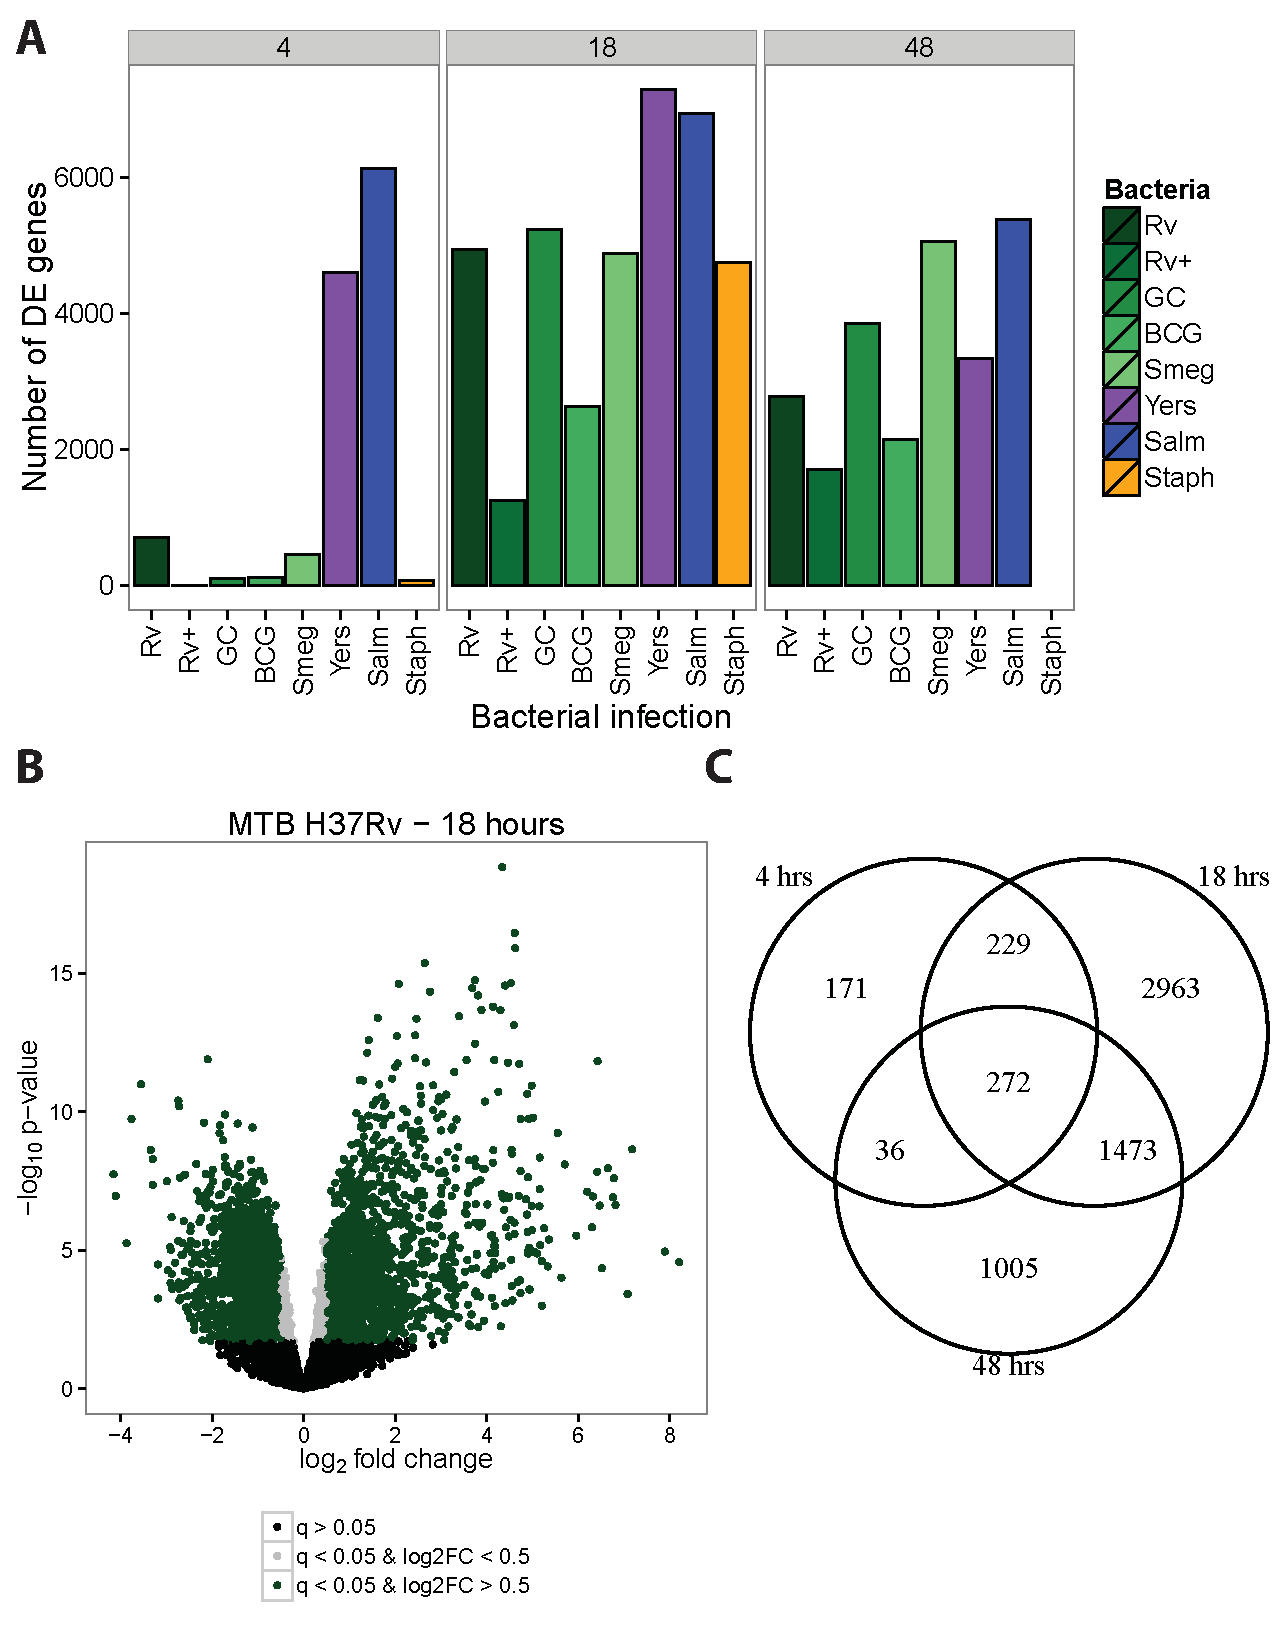
\includegraphics[width=5in]{img/ch02/fig-01-differential-expression.pdf}
\caption[Differential expression analysis.]{\textbf{Differential
    expression analysis.} We tested for differentially expressed genes
  for each bacterial infection by comparing it to its time-matched
  control. (A) We classified genes with q-value \textless{} 5\% as
  differentially expressed. The mycobacteria are labeled in shades of
  green. (B) As expected, there were large transcriptional changes 18
  hours post-infection with MTB H37Rv. Genes with q-value \textless{}
  5\% and absolute log\textsubscript{2} fold change greater than 0.5
  are labeled green, those with q-value \textless{} 5\% and absolute
  log 2 fold change less than 0.5 are labeled grey, and
  non-differentially expressed genes are labeled black. (C) The
  overlap in differentially expressed genes identified at 4, 18, and
  48 hours post-infection with MTB H37Rv.  }
\label{fig:differential-expression}
\end{figure}


\subsection{Joint analysis identifies bacteria-specific response
genes}\label{joint-analysis-identifies-bacteria-specific-response-genes}

In order to learn about variation in the innate immune response to
bacterial infection, we identified genes whose regulation was altered
by treatment with specific bacteria at specific timepoints. We first
used a naïve approach whereby we determined all the pairwise overlaps
between lists of DE genes across treatments (Supplementary Table
\ref{tab:ch02-s7}). The caveat of this strategy is that incomplete
power can result in overestimating the difference between
treatments. In order to account for incomplete power to detect DE
genes when performing multiple pairwise comparisons, we performed a
joint Bayesian analysis, which we implemented using the R/Bioconductor
package Cormotif \citep{Wei2015} (see Methods for more details). Using
this approach, we classified genes into regulatory patterns based on
their expression levels following each of the bacterial infections.

First, we examined the data across all the bacteria-time combinations.
Initially we built a model that classified genes into one of 14
separate patterns based on their expression levels after each
infection relative to their expression level in the non-infected
control (Supplementary Fig. \ref{fig:joint-all-k14}). However, we
found that a model with only six expression patterns
(Fig. \ref{fig:joint-all}; Supplementary Tables
\ref{tab:ch02-s3},\ref{tab:ch02-s4}), where a subset of the original
14 patterns are combined, is more intuitive from a biological
perspective; thus we proceeded with the reduced model. Broadly
speaking, we classified genes as responding in the early, middle, or
late stages of infection, and we characterized the response as
temporary or sustained. Pattern ``non-DE'' includes 4,245 genes whose
expression levels were unchanged in all the experiments. Pattern
``Yers-Salm'' includes 1,414 early response genes whose expression
levels changed at four hours post-infection with either
\emph{Y. pseudotuberculosis} or \emph{S. typhimurium}, but not after
infection with other bacteria. The genes in this pattern are enriched
for gene ontology (GO) annotations related to type I interferon
signaling (e.g. \emph{SP100}, \emph{IFI35}, \emph{STAT2}), antigen
presentation (\emph{HLA-A}, \emph{PSME1}, \emph{CTSS}), and apoptosis
(\emph{CASP8}, \emph{TRADD}, \emph{FADD}) (Supplementary Table
\ref{tab:ch02-s5}). Pattern ``18 h'' includes 3,201 middle response
genes whose expression levels changed exclusively at 18 hours
post-infection in response to all bacteria and is enriched for GO
annotations related to apoptosis (e.g. \emph{E2F1}, \emph{TP53},
\emph{WWOX}). Pattern ``48 h'' includes 1,204 late response genes
whose expression levels changed at 48 hours and is enriched for GO
annotations related to phagocytosis (e.g. \emph{MFGE8},
\emph{COLEC12}) and tumor necrosis factor-mediated signaling
(e.g. \emph{STAT1}, \emph{TRAF2}, \emph{TNFRSF14}). Pattern ``18 \& 48
h'' includes 1,926 middle-sustained response genes whose expression
levels changed at 18 and 48 hours and is enriched for GO annotations
related to the regulation of phagocytosis (e.g. \emph{CD36}) and TLR
signaling (\emph{TLR1}, \emph{TLR2}, \emph{MYD88}). Lastly, pattern
``All'' includes 738 early-sustained genes whose expression levels
changed after infection with all the bacteria across all three
timepoints and is enriched for GO annotations related to type I
interferon signaling (e.g. \emph{IRF1}, \emph{SOCS1}, \emph{IFIT3}),
cytokine secretion (\emph{TNF}, \emph{IL10}, \emph{LILRB1}), and
apoptosis (e.g. \emph{IRF7}, \emph{BCL2A1}, \emph{MCL1}).

\begin{figure}
\centering 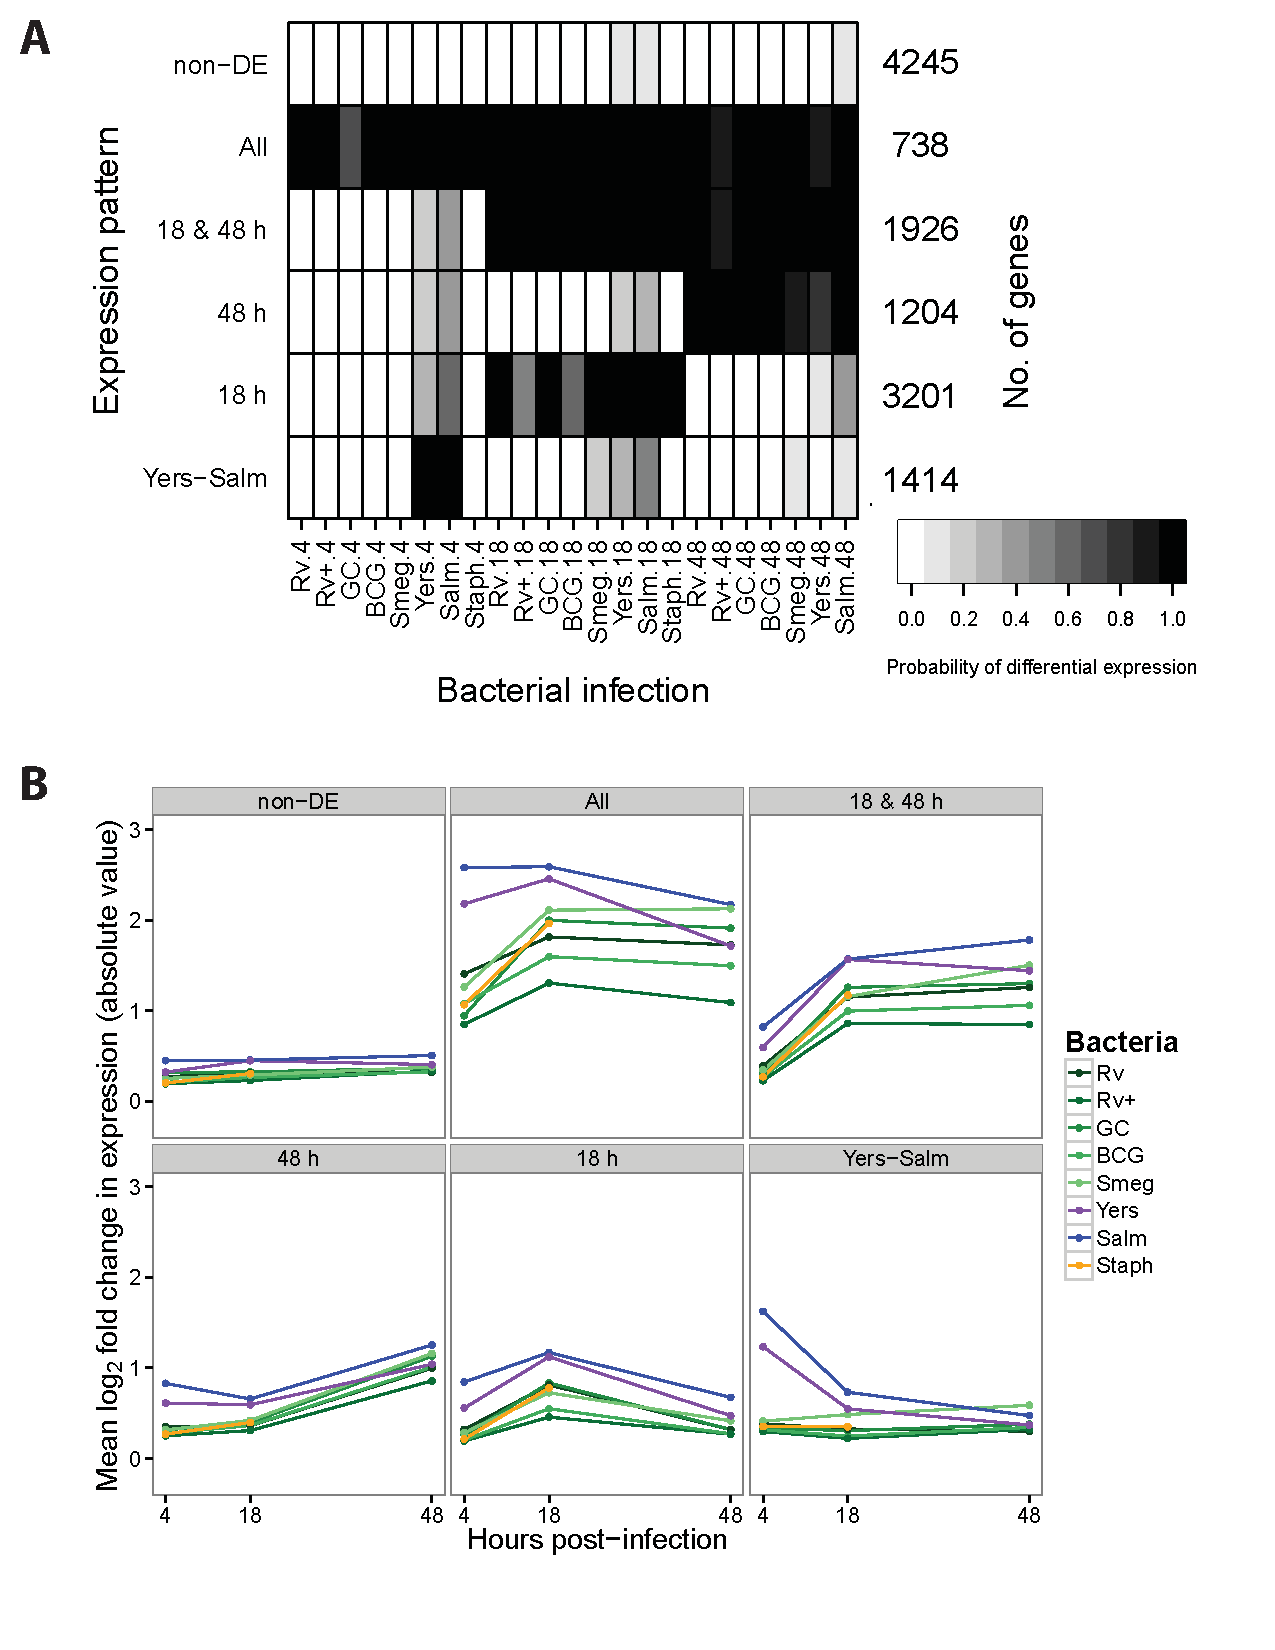
\includegraphics[width=5in]{img/ch02/fig-02-joint-all.pdf}
\caption[Joint Bayesian analysis.]{\textbf{Joint Bayesian analysis.}
  (A) Joint analysis of gene expression data from all three timepoints
  with Cormotif \citep{Wei2015} identified six expression patterns:
  ``non-DE'', ``Yers-Salm'', ``18 h'', ``48 h'', ``18 \& 48 h'', and
  ``All''. The shading of each box represents the posterior
  probability that a gene assigned to the expression pattern (row) is
  differentially expressed in response to infection with a particular
  bacteria (column), with black representing a high posterior
  probability and white a low posterior probability. (B) Each data
  point is the mean log\textsubscript{2} fold change in expression
  (absolute value) in response to infection with the given bacteria
  for all the genes assigned to the particular expression pattern.}
\label{fig:joint-all}
\end{figure}

Next, we tested for more specific patterns by performing Cormotif
separately on the data from the middle (18 h) and late (48 h) stages
of infection. At 18 hours post-infection, we identified five separate
expression patterns (Fig. \ref{fig:joint-18h}; Supplementary Tables
\ref{tab:ch02-s3},\ref{tab:ch02-s4}). Pattern ``non-DE'' includes
5,268 genes whose expression levels were unchanged across all
infections. Pattern ``All'' includes 4,424 genes whose expression
levels were affected by all infections (e.g. \emph{IL24}, \emph{IRF2},
\emph{TLR2}). Pattern ``MTB'' includes 177 genes whose expression
levels changed specifically in response to infection with mycobacteria
(e.g. \emph{NCF2}, \emph{TNFSF13}, \emph{CSF1}). These genes had a
high posterior probability of being DE 18 hours after infection with
MTB H37Rv, heat-killed H37Rv, MTB GC1237, and BCG.  Furthermore, the
gray shading for \emph{M. Smegmatis} (Fig. \ref{fig:joint-18h}A)
signified an intermediate posterior probability for DE. In essence,
this pattern is a merger of two sets of genes that were not large
enough to be separated: one set that was DE across all five
mycobacteria and another that was only DE after infection with the MTB
strains and the closely-related BCG, but not
\emph{M. Smegmatis}. Pattern ``Virulent'', in contrast, includes 1,165
genes whose expression levels were less strongly changed after
infection with heat-inactivated MTB H37Rv or the attenuated vaccine
strain BCG compared to the other bacteria (e.g.  \emph{IL1R1},
\emph{IRF1}, \emph{PILRB}). Also the genes in this category only have
an intermediate probability of responding to the non-pathogenic
\emph{M. smegmatis}. Lastly, pattern ``Yers-Salm'' includes 1,694
genes whose expression levels changed preferentially after infection
with \emph{Y. pseudotuberculosis} or \emph{S.  typhimurium}
(e.g. \emph{TLR8}, \emph{TGFB1}, \emph{IL18}).

\begin{figure}
\centering 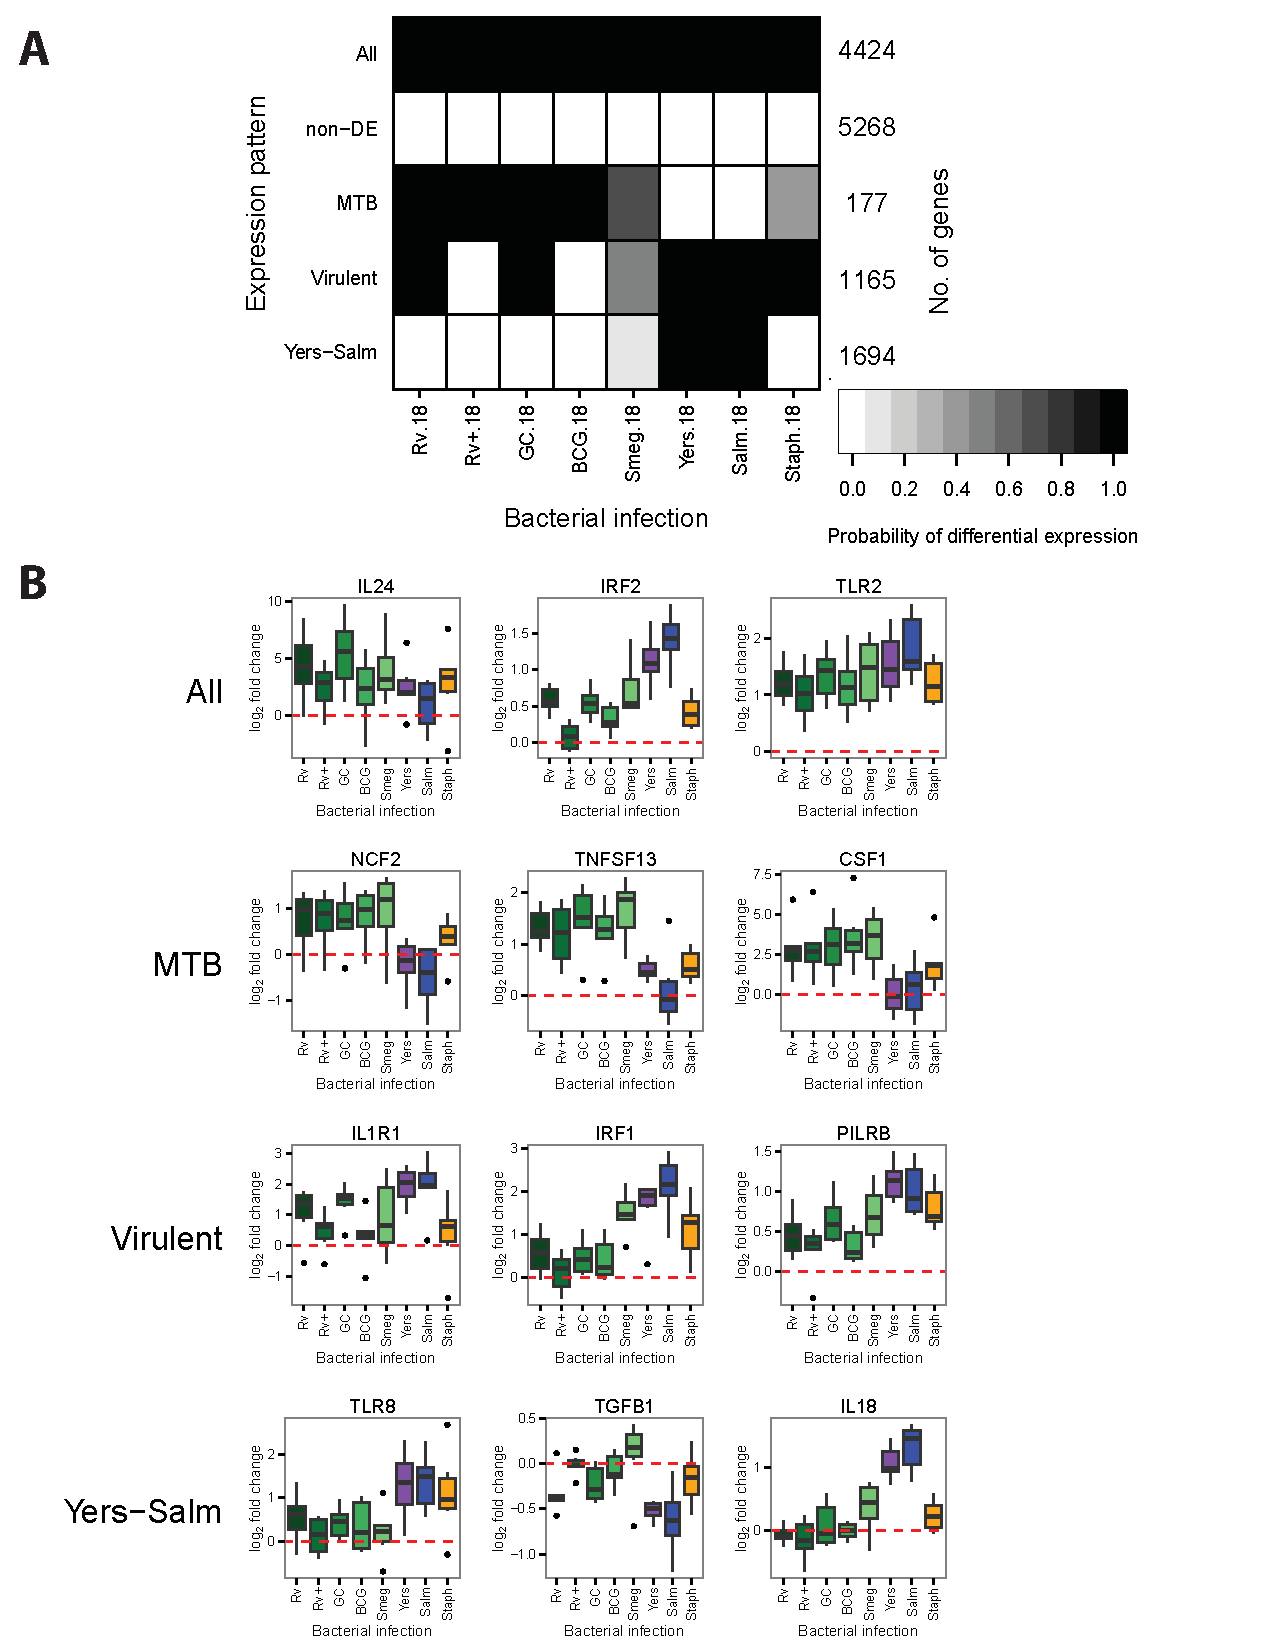
\includegraphics[width=5in]{img/ch02/fig-03-joint-18h.pdf}
\caption[Joint Bayesian analysis - 18 hours
  post-infection.]{\textbf{Joint Bayesian analysis - 18 hours
    post-infection.} (A) Joint analysis of gene expression data from
  18 hours post-infection with Cormotif identified five expression
  patterns: ``Yers-Salm'', ``Virulent'', ``MTB'', ``non-DE'', and
  ``All''. (B) Example genes from the different expression patterns.}
\label{fig:joint-18h}
\end{figure}

At 48 hours post-infection, we also discovered five expression
patterns (Fig. \ref{fig:joint-48h}; Supplementary Tables
\ref{tab:ch02-s3},\ref{tab:ch02-s4}). While many of the patterns have
similar specificities to those observed at 18 hours post-infection,
there is only little overlap across timepoints with respect to the
genes comprising the patterns. For example, pattern ``Yers-Salm'' at
48 hours includes 1,582 genes whose expression levels changed strongly
after infection with \emph{Y. pseudotuberculosis} or
\emph{S. typhimurium} (e.g. \emph{HLA-DPB1}, \emph{IL10RB},
\emph{CD248}), but only 263 of these genes are also in the
corresponding pattern when we considered the data from the 18 hour
timepoint. Similarly, at the 48 hour timepoint, pattern ``MTB''
includes 288 genes whose expression levels changed preferentially
after infection with mycobacteria (e.g. \emph{CCL1}, \emph{ATP6V1A},
\emph{IL27RA}), but only 33 of these genes are in the corresponding
pattern at the 18 hour timepoint. Pattern ``Virulent'' includes 14
genes whose expression levels were not changed after infection with
heat-inactivated MTB H37Rv or the attenuated vaccine strain BCG
(e.g. \emph{MAP3K4}, \emph{SEMA4G}, \emph{BTG1}), and only one of
these also belongs to the pattern ``Virulent'' at 18 hours
post-infection.

\begin{figure}
\centering 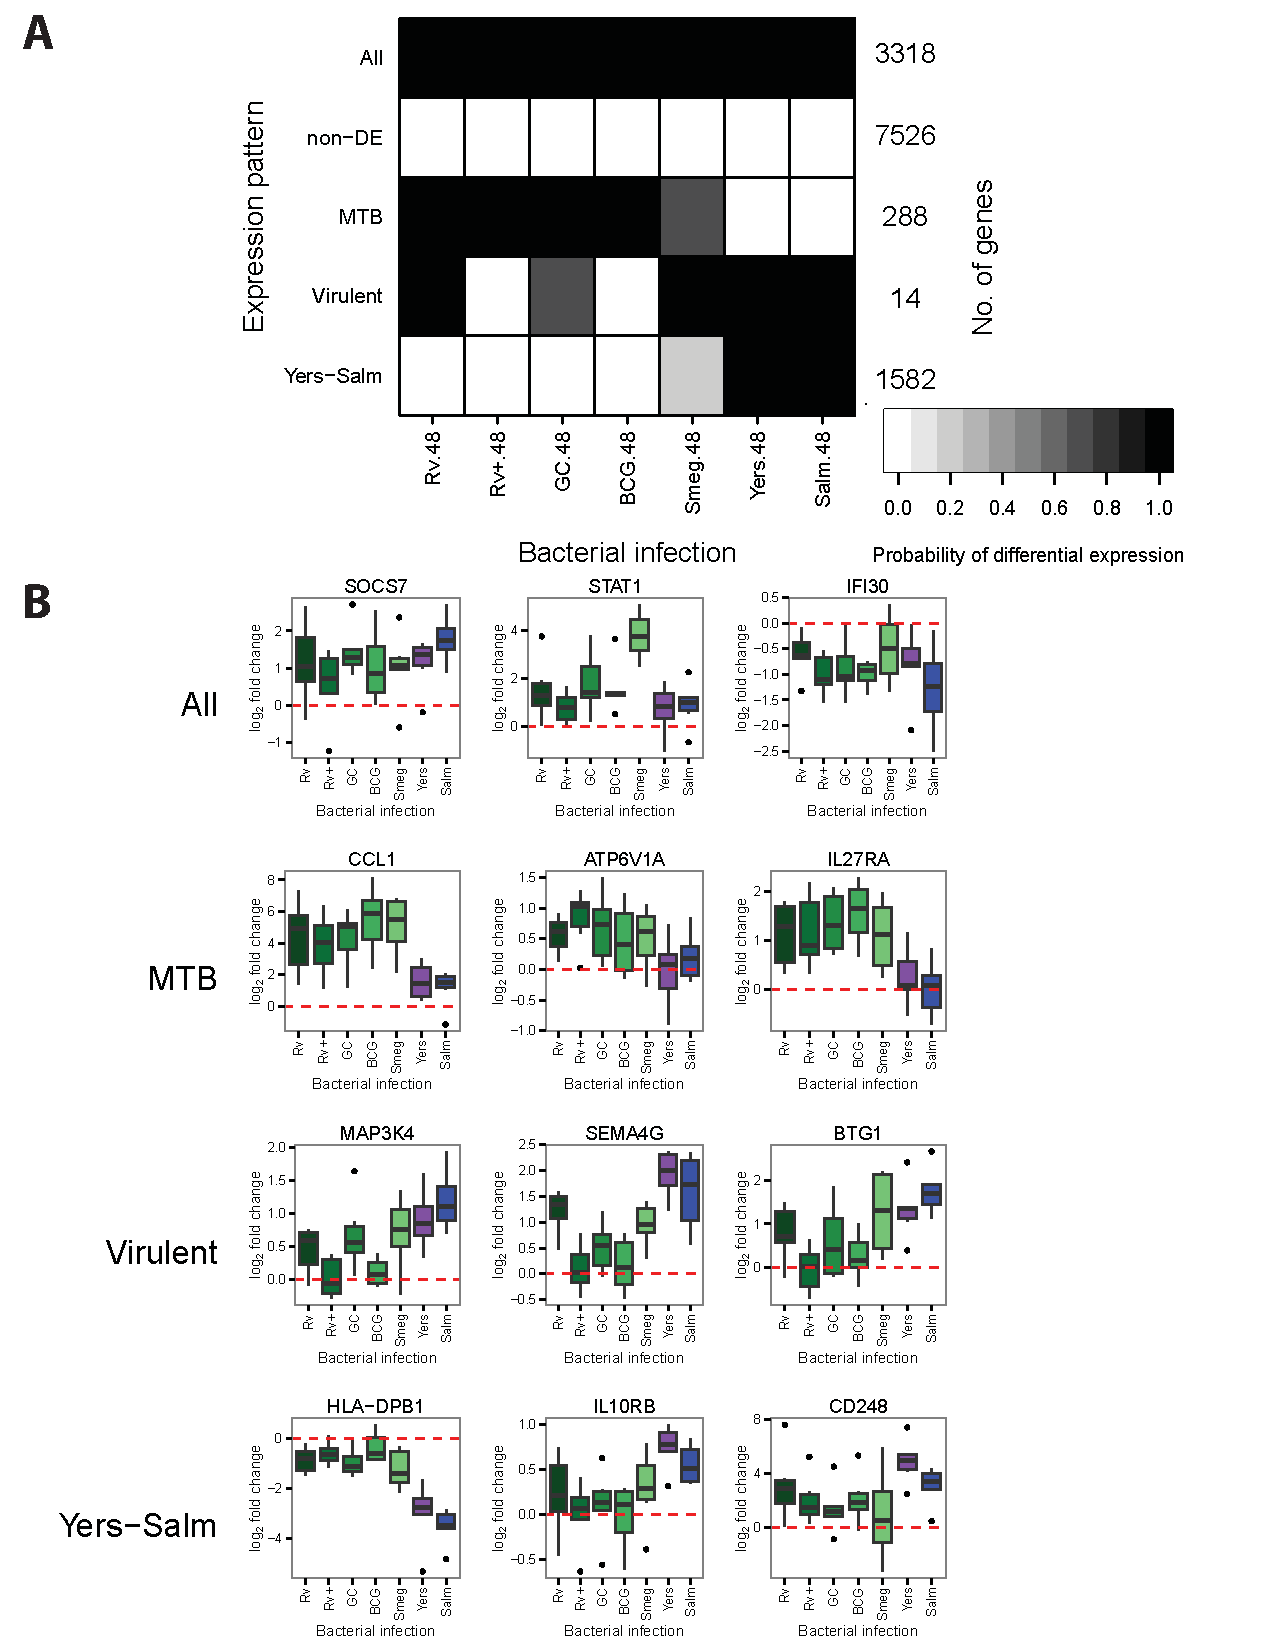
\includegraphics[width=5in]{img/ch02/fig-04-joint-48h.pdf}
\caption[Joint Bayesian analysis - 48 hours
  post-infection.]{\textbf{Joint Bayesian analysis - 48 hours
    post-infection.} (A) Joint analysis of gene expression data from
  48 hours post-infection with Cormotif identified five expression
  patterns: ``Yers-Salm'', ``Virulent'', ``MTB'', ``non-DE'', and
  ``All''. (B) Example genes from the different expression patterns.}
\label{fig:joint-48h}
\end{figure}

\subsection{Infection-induced response eQTLs are shared across
bacterial
infections}\label{infection-induced-response-eqtls-are-shared-across-bacterial-infections}

Using the gene expression patterns we identified by applying the joint
analysis approach, we investigated the specificity of previously
identified response eQTLs to infection with MTB H37Rv
\citep{Barreiro2012}. Since the response eQTLs were identified at 18
hours post-infection, we investigated the distribution of genes
associated with response eQTLs among the five patterns we found at
that timepoint (Fig. \ref{fig:response-eqtl}A). Only one gene
associated with a response eQTL was also DE specifically in response
to MTB (\emph{CMAS}). Otherwise, most of the response eQTL-associated
genes were classified as either DE following infection with all
bacteria or not DE in any infection. That a large proportion of the
genes associated with response eQTLs were not DE in any of these
experiments is likely due to the fact that the eQTL study was
performed in dendritic cells whereas our data were collected from
macrophages. Overall, our observations suggest that most of the
previously identified response eQTLs are genetic variants that affect
the human innate immune response to bacterial infection in general,
and not specifically the response to MTB H37Rv.

To provide further broad support for the interpretation that the
response eQTL genes are important for the innate response to bacterial
nfection in general, we considered the log\textsubscript{2} fold
change in expression values following infection
(Fig. \ref{fig:differential-expression}). For each gene, we calculated
the mean log\textsubscript{2} fold change in expression level across
the eight bacterial infections at the 18 hour timepoint. Next, we
compared the absolute values of the log\textsubscript{2} fold change
in expression between genes associated with response eQTLs, genes
associated with general eQTLs (i.e.~genes associated with an eQTL pre-
and post-infection), and genes not found to be associated with an
eQTL.  Since there was a large difference in the number of genes in
these three classes, we subsampled genes from each and calculated the
mean of the absolute values (and repeated this process 1000 times). We
found that the expression level of genes associated with response
eQTLs is altered to a larger degree (significantly higher effect size;
\emph{P} \textless{} 2.2 x e\textsuperscript{-16};
Fig. \ref{fig:response-eqtl}B) following infection compared to the
genes in the other two classes.

\begin{figure}
\centering
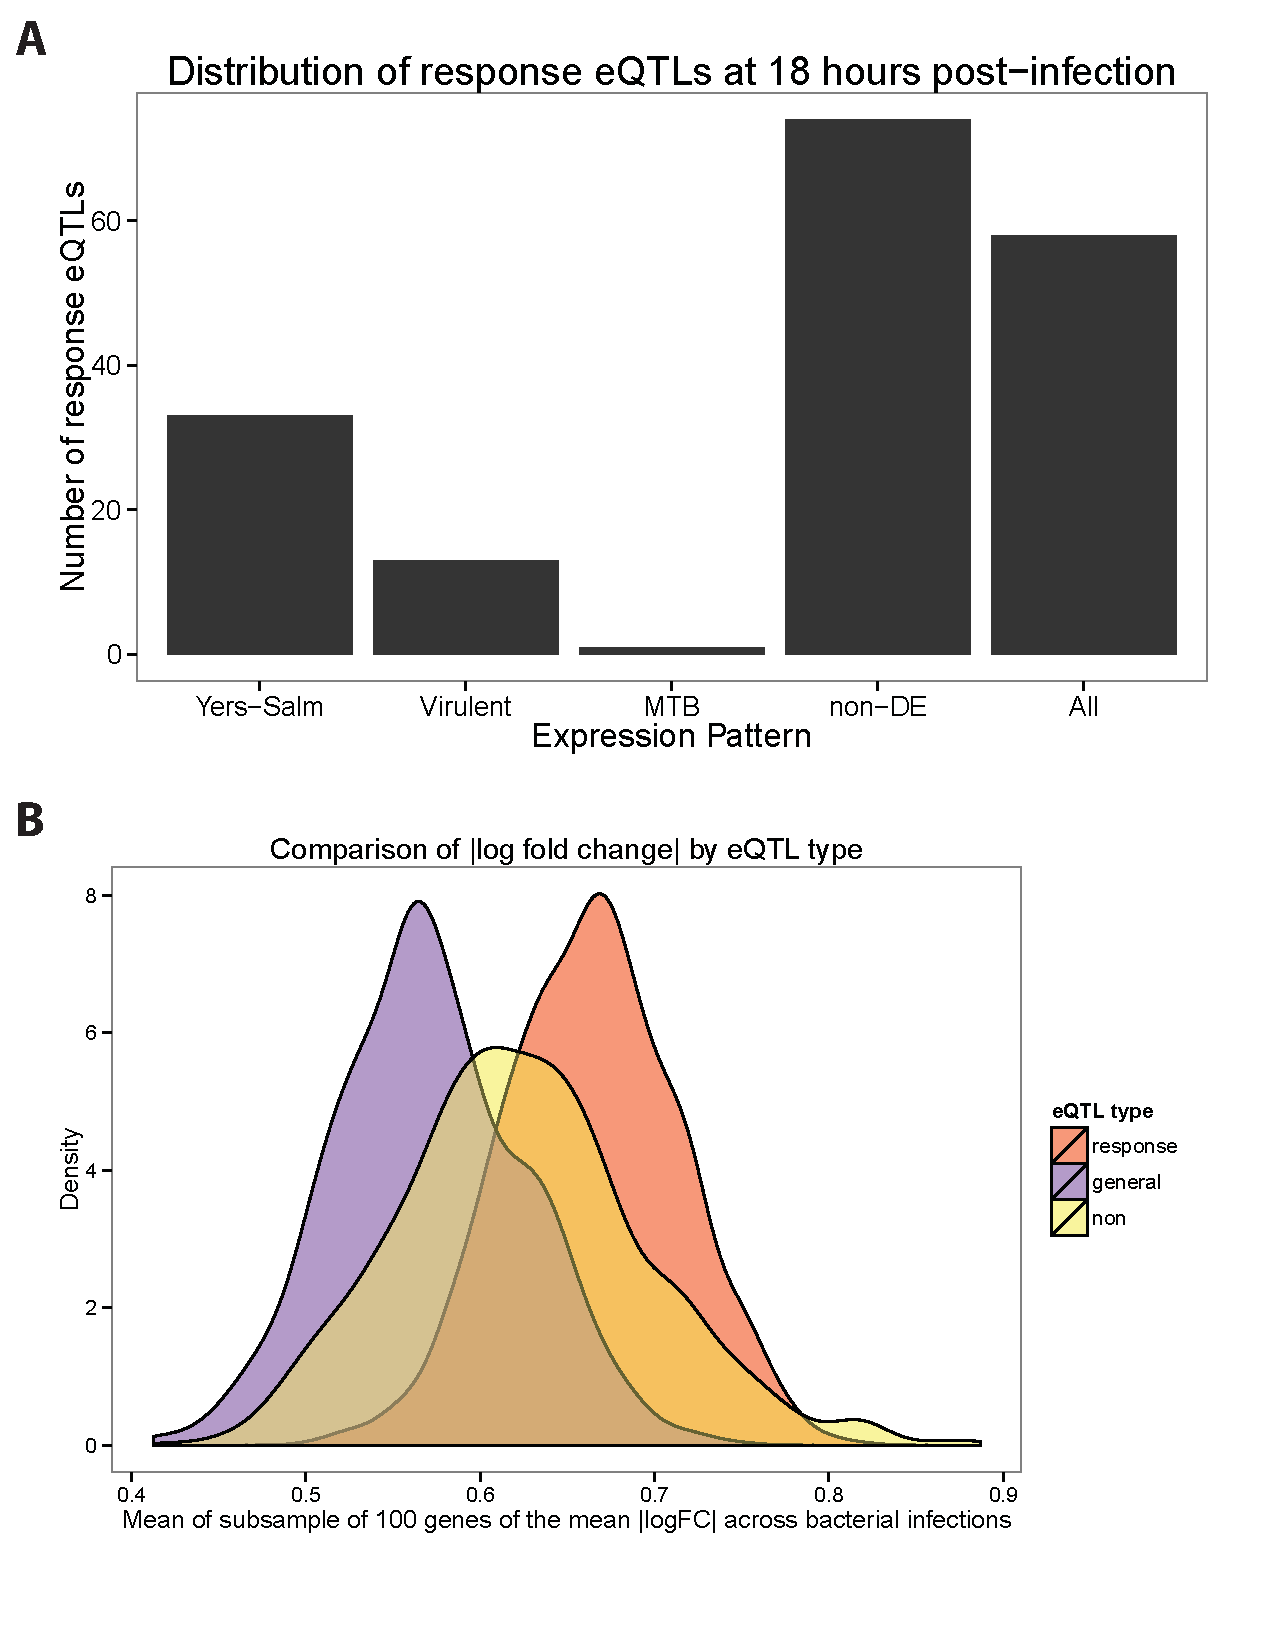
\includegraphics[width=5in]{img/ch02/fig-05-response-eqtl.pdf}
\caption[Response eQTLs at 18 hours post-infection.]{\textbf{Response
    eQTLs at 18 hours post-infection.} (A) We counted the number of
  response eQTLs from Barreiro et al. \citep{Barreiro2012} (179 out of
  the 198 were also expressed in our study) in each of the five gene
  expression patterns at 18 hours post-infection
  (Fig. \ref{fig:joint-18h}).  (B) We compared the mean
  log\textsubscript{2} fold change in expression across the 8
  bacterial infections at the 18 hour timepoint for three classes of
  genes: response eQTL genes (red), general eQTL genes (purple), and
  non-eQTL genes (yellow) (see Methods for details).  }
\label{fig:response-eqtl}
\end{figure}

\section{Discussion}\label{ch02-discussion}

\subsection{Bayesian analysis identified mycobacteria-specific
response
genes}\label{bayesian-analysis-identified-mycobacteria-specific-response-genes}

In order to identify general and treatment-specific gene regulatory
responses, we performed a joint Bayesian analysis of the data using
Cormotif \citep{Wei2015}. By jointly analyzing the data, as opposed to
comparing overlaps between independent lists of differentially
expressed genes generated using an arbitrary cutoff, we minimized the
identification of specific responses due to false negatives
(i.e.~genes that appear to be differentially expressed in response to
a subset of bacterial infections when in reality the response is
similar across all the infections). Similar to previous observations
\citep{Huang2001, Boldrick2002}, we found a large core transcriptional
response to infection. However, we also identified a novel subset of
genes whose regulation is preferentially altered in response to
infection with mycobacteria but not to the other bacteria we
tested. Since these responses are unique to infection with
mycobacteria (at least in the context of our study design), they may
be promising candidates for future studies that focus on the
mechanisms by which mycobacteria successfully subvert the human innate
immune response. Since this study does not extend to investigation of
mechanisms, we do not have empirical data with which to prioritize
such possible candidate genes. Yet, the reported functions of many of
these genes often suggest mechanisms that are relevant, and often
quite specific, to MTB infection. Prioritizing candidate genes in this
way is not statistically valid, and one can argue (and indeed, this
has been shown \citep{Pavlidis2012}) that any list of genes can be
scrutinized to yield ``interesting relevant stories''. We therefore
offer these details in the context of a discussion (rather than
``results''), to provide one set of alternative explanations for our
findings, and generate ideas for further investigations.

For example, when we focused on the mycobacteria-specific regulatory
response 18 hours post-infection, we noticed an intriguing number of
genes that are involved in phagosome maturation (Supplementary
Fig. \ref{fig:phago}). Broadly speaking, phagocytosed bacteria are
killed by vesicular proton pumps, which lower the pH inside the
phagosome, and lysosomal fusion. This process occurs once a phagosome
has matured through a series of steps mediated by the exchange of Rab
GTPases \citep{Vergne2004, Mortellaro2009}. A unique property of
mycobacteria is their ability to survive inside the macrophage by
inhibiting phagosome maturation \citep{Hestvik2005}. As part of this
strategy, the bacterium recruits \emph{RAB22A} to MTB-containing
phagosomes \citep{Roberts2006}. Indeed, we found the \emph{RAB22A}
gene to be upregulated in response to infection with mycobacteria
(Supplementary Table \ref{tab:ch02-s4}). Similar GTPases whose
regulation was altered following mycobacterial infections include
\emph{RAP2A} (upregulated), \emph{RAB3A} and \emph{RAB33A} (both
downregulated). In addition, the vesicular (v)-ATPase subunit
\emph{ATP6V1D} was exclusively upregulated in response to
mycobacterial infection. Thus, the mycobacteria-specific response we
identified includes genes putatively involved in mycobacteria-specific
survival mechanisms.

An additional intriguing example involves the \emph{NCF2} gene. This
is a potential candidate gene whose expression level was affected
specifically by infection with mycobacteria at 18 hours
post-infection.  Neutrophil cytosolic factor 2 (\emph{NCF2}, also
known as \emph{p67phox}) is a subunit of the phagocyte NAPDH oxidase,
which is responsible for generating reactive oxygen species used to
fight intracellular pathogens \citep{Ehrt2001, Myers2003, Babior2004,
  Bustamante2011, Kim2011c, Deffert2014}. These reactive oxygen
species may also serve a signaling role in activating other immune
cell types to ensure proper granuloma formation and killing of
mycobacteria \citep{Deffert2014a}. Loss-of-function mutations in
subunits of the NAPDH oxidase cause chronic granulomatous disease
(CGD) \citep{Deffert2014}, which is characterized by the formation of
granulomas throughout the body due to the inability of phagocytes to
kill the ingested pathogens.  In contrast to wild type animals, mice
with mutations in subunits of the phagocyte NAPDH oxidase develop
tuberculosis after infection with the vaccine strain, BCG
\citep{Deffert2014a}. Humans who are administered the vaccine before
being diagnosed with CGD also develop the disease \citep{Deffert2014}.

At 48 hours post-infection (Fig. \ref{fig:joint-48h}), the
mycobacteria-specific response was enriched with genes annotated
(based on GO) as having a role in ``response to vitamin D''
(Supplementary Table \ref{tab:ch02-s5}; Supplementary
Fig. \ref{fig:vitD}). Individuals with low circulating levels of
vitamin D are more susceptible to developing tuberculosis
\citep{Zodpey2007, Nnoaham2008}, and vitamin D has been investigated
as a supplemental therapy for the treatment of tuberculosis, though
with mixed results \citep{Martineau2007, Lucas2014, Xia2014,
  Kearns2015}. Vitamin D has been found to be important for innate
immune cells to fight MTB \citep{Liu2006, Verway2013, Xu2014};
however, it is also an important pathway for generic bactericidal
activity \citep{Hewison2011}. Consistent with its role in the innate
immune response, both the enzyme that converts vitamin D to its active
form (\emph{CYP27B1}) and its receptor (\emph{VDR}) are upregulated in
response to any of the infections (pattern ``All'';
Fig. \ref{fig:joint-48h}). Yet, the regulation of other genes involved
in the response to vitamin D was only affected by infection with MTB.
\emph{PIM1}, a serine/threonine kinase that binds the VDR and enhances
transcription of its target genes \citep{Maier2012}, is upregulated in
response to the mycobacteria (pattern ``MTB'',
Fig. \ref{fig:joint-48h}). Interestingly, the increased expression
level of \emph{PIM1} in T-cells was successfully used in a six-gene
classifier of patients with active versus latent TB infections
\citep{Jacobsen2011}. Another gene, the chemokine \emph{CXCL10} (also
known as interferon gamma-induced protein 10 or IP-10), is also
upregulated in response to mycobacterial infection (pattern ``MTB'',
Fig. \ref{fig:joint-48h}). Discordant with the observed increase in
expression of \emph{CYP27B1}, \emph{VDR}, and \emph{PIM1} in response
to infection, treatment with vitamin D usually leads to the reduction
of \emph{CXCL10} expression and secretion in multiple cell types
\citep{Gysemans2005, Adorini2005, Scolletta2013}. In fact,
supplementation with vitamin D decreased serum levels of CXCL10 in TB
patients \citep{Coussens2012}. This suggests that the immunosuppresive
effect of vitamin D signaling is insufficient to overcome the
pro-inflammatory response to mycobacterial infection. This observation
is in concordance with past studies which found increased expression
of \emph{CXCL10}, as well as increased secretion level from
macrophages, following infection with MTB \citep{Zhu2006,
  Verway2013}. Interestingly, a polymorphism in \emph{CXCL10} was
found to be associated with susceptibility to tuberculosis in a
Chinese population \citep{Tang2009, Azad2012}. Overall, these
observations provide support for the importance of vitamin D signaling
for specifically fighting mycobacterial infections.

Another gene of interest from the mycobacteria-specific expression
pattern at 48 hours post-infection is chemokine (C-C motif) ligand 1
(\emph{CCL1}), which stimulates migration of human monocytes
\citep{Miller1992} (Fig. \ref{fig:joint-48h}B). Thuong et
al. identified \emph{CCL1} as being induced to a greater extent in
MTB-infected macrophages (4 hours post-infection) isolated from
individuals with pulmonary TB compared to macrophages from individuals
with latent TB infections \citep{Thuong2008}. Put together, our
observations and those of Thuong and colleagues suggest that
\emph{CCL1} is involved in the pathogenesis of TB. Further supporting
this notion, Thuong et al. also found a genetic association between
variants in the \emph{CCL1} region and TB susceptibility
\citep{Thuong2008}. However to date, subsequent genetic association
studies investigating \emph{CCL1} have reported mixed results
\citep{Tang2011, Ozdemir2013}.

One caveat of the joint Bayesian analysis is that we were not able to
classify genes into unusual patterns (because this approach can only
discover expression patterns shared by a large number of genes and, by
definition, only few genes fall into ``unusual'' patterns). For
example, unusual patterns of interest include changes in expression
specifically in response to some but not all of the mycobacterial
infections. One gene that satisfied this pattern is the dual
specificity phosphatase 14 (\emph{DUSP14}). We specifically examined
the expression data for this gene because it was previously associated
with an MTB infection response eQTL in dendritic cells
\citep{Barreiro2012}, and consequently when the eQTL results were used
as a prior - \emph{DUSP14} was found to be significantly associated
with TB susceptibility. Moreover, knocking down \emph{DUSP14}
expression via siRNA in murine macrophages resulted in a lower
bacterial load 90 hours post-infection with MTB H37Rv
\citep{Jayaswal2010}. In our joint Bayesian analysis, \emph{DUSP14}
was not classified as one of the genes whose regulation was altered in
response to infection with mycobacteria. Yet, \emph{DUSP14} was
upregulated at 18 hours post-infection with MTB H37Rv (q-value: 16\%),
MTB GC1237 (q-value: 3\%), and BCG (q-value: 9\%); and downregulated
post-infection with \emph{S. typhimurium} (q-value: 9\%)
(Supplementary Fig. \ref{fig:dusp14}). Thus, our data lends further
support for the role of \emph{DUSP14} as a TB susceptibility gene.

\subsection{Little evidence for strain-specific transcriptional
response to
infection}\label{little-evidence-for-strain-specific-transcriptional-response-to-infection}

There are six major families of MTB that differ in their geographic
distribution and virulence \citep{Gagneux2006, Comas2009}. Strains
from these families are known to differ in their growth rates inside
macrophages \citep{Li2002}, expression levels of bacterial genes
\citep{Homolka2010, Rose2013}, and cell wall lipid composition
\citep{Krishnan2011}. Previous studies have found that different MTB
strains induce different innate immune responses in human cell lines
and other infection models \citep{Coscolla2010}. A dominate narrative
is that MTB strains from East Asia, referred to as the Beijing family
(Gagneux et al. classified it as MTB lineage 2 \citep{Gagneux2006}),
are more virulent because they induce a lower proinflammatory immune
response compared to the common laboratory strains \citep{Manca2001,
  Manca2004, Reed2004, Tanveer2009, Wang2010}. However, other studies
have reported the opposite, namely that Beijing strains induce a
larger proinflammatory response \citep{Chacon-Salinas2005}, or a
conflicting response in which various pro- and anti-inflammatory
cytokines are differentially regulated \citep{Rocha-Ramirez2008,
  Koo2012} compared to laboratory strains.

In our study, albeit with a small sample size, we found no marked
differences between the transcriptional response to infection with MTB
H37Rv or MTB GC1237, a Beijing strain (Supplementary
Fig. \ref{fig:Rv-v-GC}; Supplementary Table
\ref{tab:ch02-s8}). Furthermore, the pro-inflammatory cytokines
\emph{TNF} and \emph{IL6} and the anti-inflammatory cytokine
\emph{IL10} were strongly upregulated in response to both strains of
MTB (Supplementary Fig. \ref{fig:ex-cytokines}). This observation is
in concordance with Wu et al., who also reported no apparent
difference in the transcriptional response of THP-1 cells to infection
with MTB H37Rv versus multiple Beijing strains \citep{Wu2012}. Thus
the increased virulence of the Beijing family of MTB strains may be
due to mechanisms not assayed in this study such as
post-transcriptional effects, cell-cell signaling, and environmental
stimuli. It should be noted, however, that not all Beijing strains are
equally virulent \citep{Dormans2004, Sinsimer2008} and that MTB H37Rv
is a laboratory-adapted strain that has evolved independently in
different laboratories \citep{Ioerger2010}.

\subsection{Differences in response to virulent versus attenuated
pathogens are not
mycobacteria-specific}\label{differences-in-response-to-virulent-versus-attenuated-pathogens-are-not-mycobacteria-specific}

To better understand the interaction between MTB and macrophages, we
included in our study both virulent mycobacteria (MTB strains H37Rv
and GC1237) and attenuated mycobacteria (heat-inactivated MTB H37Rv
and the vaccine strain BCG). Overall, the response to infection with
either virulent or attenuated mycobacteria was similar
(Fig. \ref{fig:joint-18h},\ref{fig:joint-48h}). This observation was
unsurprising because it has been previously demonstrated that
infections with inactivated pathogens (in fact, even individual
pathogen components) are able to largely recapitulate the
transcriptional response to infection \citep{Huang2001, Boldrick2002,
  Nau2002, Jenner2005}. In other words, as expected, the
transcriptional response to infection is largely driven by the
antigens present.

Yet, the responses to inactivated pathogens or individual pathogen
components in past studies were not identical to the responses to live
pathogens, suggesting a potential role for bacterial manipulation of
the immune response. For example, it is known that BCG lacks the locus
containing the ESX-1 secretion system, which is critical for MTB
virulence \citep{Behr1999, Pym2002, Hsu2003, Simeone2009}. In our
study we also observed differences between the response to virulent
and attenuated mycobacteria. Specifically, there are 1,165 genes in
the expression pattern ``Virulent'' at 18 hours post-infection
(Fig. \ref{fig:joint-18h}) and 14 genes that comprise of the
``Virulent'' pattern at 48 hours post-infection
(Fig. \ref{fig:joint-48h}). Importantly, these genes are also
differentially expressed in response to the other virulent infections
in our study, and thus they are not specifically due to the
manipulations of the host cell by virulent mycobacteria.

We attempted to identify a gene expression pattern that specifically
represented differences in virulence only in the mycobacteria, yet we
never saw such a pattern. It is important to note that had we simply
performed a simple pairwise analysis of the overlap of DE genes
between MTB and BCG infections, our results would be quite different
(Supplementary Table \ref{tab:ch02-s7}). Yet, a pairwise analysis is
misleading in the context of the entire study. Indeed, by accounting
for incomplete power by using the joint Bayesian model and including
other bacterial species, we avoided attributing many differentially
expressed genes specifically to the differences in the immune evasion
mechanisms used by MTB and BCG.  We conclude that either a larger
sample size or a different experimental system is required to find
specific differences between the response to infection with MTB and
BCG.

\subsection{Previously identified response eQTLs affect response to
bacterial infection in
general}\label{previously-identified-response-eqtls-affect-response-to-bacterial-infection-in-general}

In a previous study, we identified response eQTLs that were associated
with gene expression levels in MTB-infected human dendritic cells. We
investigated the expression pattern of genes associated with the
response eQTLs in our study. Using the five expression patterns
identified by the joint Bayesian analysis at 18 hours post-infection,
we examined the distribution of response eQTL genes and discovered
that these genes were not enriched in the mycobacteria-specific
expression pattern (Fig. \ref{fig:response-eqtl}A). Instead, many were
differentially expressed across all the infections (pattern
``All''). Thus, response eQTLs modulate the inter-individual response
to infection with diverse types of bacteria.  That said, one gene was
both associated with a response eQTL and specifically differentially
expressed following mycobacterial infection.  Though this result does
not represent a significant enrichment of response eQTL genes among
those whose regulation was affected specifically by infection with
MTB, the identity of the gene renders the observation
intriguing. \emph{CMAS} (cytidine monophosphate N-acetylneuraminic
acid synthetase), is an enzyme that is involved in the processing of
sialic acid, which is then added to cell surface glycoproteins and
glycolipids. Glycoproteins are known to be important in many functions
of the immune response, including initial pathogen detection
(e.g.~TLRs) and antigen presentation (e.g.~major histocompatibility
complex (MHC) molecules) \citep{Wolfert2013, Johnson2013,
  Crespo2013}. We suggest that this gene is an interesting candidate
for further understanding both MTB pathogenesis and inter-individual
susceptibility to tuberculosis.

\subsection{Conclusions}\label{ch02-conclusions}

By jointly considering data from multiple infection treatments, using
a variety of bacteria, we have classified distinct innate immune
transcriptional response patterns. The most inclusive pattern was a
response to all the bacterial infections, indicating that the
receptors that bind the diverse antigens present on the different
bacteria converge to largely similar signaling pathways. We also found
an expression response pattern specific to mycobacterial infections,
the main focus of the current study. At 18 hours post-infection, the
mycobacteria response pattern includes genes involved in phagosome
maturation and the NAPDH oxidase subunit \emph{NCF2}. At 48 hours
post-infection, it includes genes involved in the response to vitamin
D and the chemokine \emph{CCL1}. We found that the response to
infection with different MTB strains was highly similar. Furthermore,
the differences we identified between the response to MTB and the
vaccine strain BCG were not mycobacteria-specific, but likely
represent a difference between the innate immune response to virulent
and non-virulent (or attenuated) pathogens. Lastly, we identified a
single gene, \emph{CMAS}, which is both associated with a response
eQTL to MTB infection, and whose regulation is altered specifically
when we infected the cells with mycobacteria. This gene is thus an
especially promising candidate for future studies of TB
susceptibility.

\section{Methods}\label{ch02-methods}

\subsection{Ethics Statement}\label{ch02-ethics-statement}

Buffy coats were obtained from healthy donors after informed consent.
The blood collection protocols were approved by both the French
Ministry of Research and a French Ethics Committee under the reference
DC-2008-68 collection 2. The blood collection was carried out in
accordance with these approved protocols by the Etablissement Français
du Sang.

\subsection{Sample collection and macrophage
differentiation}\label{sample-collection-and-macrophage-differentiation}

We collected buffy coats (\mytilde50 mL) from six healthy donors. Next
we isolated peripheral blood mononuclear cells (PBMCs) via
Ficoll-Paque centrifugation \citep{Rivero-Lezcano2012} and enriched
for monocytes via positive selection with beads containing CD14
antibodies \citep{Barreiro2012}. Then we differentiated the monocytes
into macrophages by culturing for 6-7 days in RPMI buffer supplemented
with macrophage colony-stimulating factor (M-CSF)
\citep{Tailleux2003}.

\subsection{Bacterial infection}\label{bacterial-infection}

For each bacterial infection (Table \ref{tab:bacteria}), we treated
the macrophages with a multiplicity of infection (MOI) of 2:1. After
one hour, we washed the macrophages five times with phosphate-buffered
saline (PBS) and treated them with gentamycin (50 $mu$g/$mu$L) to kill
all extracellular bacteria.  After one hour of antibiotic treatment,
we changed the medium to a lower concentration of gentamycin (5
$mu$g/$mu$L), which marked the zero timepoint of the study. We allowed
the cells to grow for 4, 18, or 48 hours before lysing them with
QIAzol Lysis Reagent and then storing them at -80° C.  We chose these
timepoints based on a previous analysis of the human transcriptional
response to infection with MTB \citep{Tailleux2008}. No data is
available for 48 hours post-infection with \emph{S.
  epidermidis}. After escaping the macrophages upon cell death,
sufficient \emph{S. epidermidis} were able to proliferate in the
gentmycin-supplemented medium to contiminate the entire well by 48
hours post-infection.

\subsection{RNA extraction, library preparation, and
sequencing}\label{rna-extraction-library-preparation-and-sequencing}

We extracted RNA using the QIAgen miRNeasy kit. There were a total of
13 batches of 12 samples each (6 individuals x 9 conditions x 3
timepoints, minus 48 hours post-infection with
\emph{S. epidermidis}). We designed the batches to maximally partition
the variables of interest (individual, condition, timepoint) in order
to minimize the introduction of biases due to batch processing
\citep{Auer2010}. To assess RNA quality, we measured the RNA Integrity
Number (RIN) with the Agilent Bioanalyzer (Supplementary Table
\ref{tab:ch02-s6}). Importantly, there were no significant differences
in the RIN (mean of 7.8 $\pm$ 2.0) between the bacterial infections or
between the timepoints (Supplementary
Fig. \ref{fig:rin-and-reads}B). In batches of 12 samples, we added
barcoded adapters (Illumina TruSeq RNA Sample Preparation Kit v2) and
sequenced 50 base pairs single end over multiple flow cells on the
Illumina HiSeq 2500.

\subsection{Mapping, counting, and
normalization}\label{mapping-counting-and-normalization}

We mapped the short reads to the human genome (hg19) using the Subread
algorithm \citep{Liao2013} and discarded those that mapped
non-uniquely.  Next, we obtained the read counts for each Ensembl
protein-coding gene (biotype: ``protein\_coding'') with the
featureCounts algorithm, which sums the reads falling in the union of
all exons of a gene and discards reads mapping to more than one gene
\citep{Liao2014}. There were no significant differences in the number
of mapped exonic reads (mean of 41.8 $\pm$ 21.2 million per sample)
between the bacterial infections or between the timepoints
(Supplementary Fig. \ref{fig:rin-and-reads}A). We removed genes with
fewer than one count per million exonic reads in fewer than six
samples.  To account for differences in the read counts at the
extremes of the distribution, we normalized the samples using the
weighted trimmed mean of M-values algorithm (TMM)
\citep{Robinson2010}.

\subsection{Differential expression
analysis}\label{differential-expression-analysis}

To assess the quality of the data, we performed principal components
analysis (PCA) of the TMM-normalized log\textsubscript{2}-transformed
counts per million (CPM). PC2 separated the samples by timepoint, but
PC1 was associated with the RIN score and the processing batch
(Supplementary Fig. \ref{fig:pca}A). After the effects of RIN score
and processing batch were removed with the function removeBatchEffect
from the limma package \citep{Ritchie2015}, PC1 separated the samples
by timepoint and PC2 separated the infected and control samples
(Supplementary Fig. \ref{fig:pca}B). We protected the variables of
interest (individual, bacteria, timepoint) when regressing the effects
of RIN score and processing batch by including them in the linear
model used by removeBatchEffect. However, the result was similar if
they were not protected since the variables of interest were
partitioned across the processing batches (Supplementary
Fig. \ref{fig:pca}C). All figures displaying expression data were
generated using the batch-corrected data.

To confirm that the transcriptional response to MTB infection in our
study was consistent with previous observations, we compared our MTB
infected samples and their time-matched controls to the MTB infected
samples and zero timepoint control from Tailleux et al., 2008
\citep{Tailleux2008}. Despite differences in the technology used to
assay gene expression (RNA-seq versus microarray) and the method used
to isolate the macrophages (positive versus negative selection), we
still observed a common transcriptional signature of infection using
PCA (Supplementary Fig. \ref{fig:tailleux2008}).

For the standard analysis, we tested for differential expression using
limma+voom \citep{Smyth2004, Smyth2005, Law2014} because it has been
shown to perform well with sufficient sample size (n \textgreater{}= 3
per condition) \citep{Rapaport2013, Soneson2013}. Based on the PCA
results, we included RIN score and processing batch as covariates in
the model. We corrected for multiple testing with the Benjamini \&
Hochberg false discovery rate (FDR) \citep{Benjamini1995} and
considered genes with q-value less than 5\% to be differentially
expressed.

Since we were interested in the shared and differential response to
infection with the different bacteria, we performed a joint Bayesian
analysis using the Cormotif algorithm \citep{Wei2015}. Cormotif shares
information across experiments, in this case infections, to identify
the main patterns of differential gene expression (which it refers to
as \emph{correlation motifs}) and assigns each gene to one of these
gene expression patterns. One caveat of the Cormotif algorithm is that
is does not distinguish the direction of the effect across
infections. In other words, a gene that is assigned to an expression
pattern could be differentially expressed in different directions
across the infections.  However, in this data set, this was rarely
observed (Supplementary Table \ref{tab:ch02-s9}).

In practice, we had to make several modifications when using Cormotif.
First, since the method was developed for microarray data, we used the
batch-corrected TMM-normalized log\textsubscript{2}-transformed CPM as
input. Second, the method assumes independence between the
experiments, and we only have one control per timepoint. However,
since this dependence will cause genes to be more likely to be either
uniformly differentially expressed across all the infections or
uniformly unchanged, this caveat is conservative to our results of
gene expression patterns that are specific to subgroups of the
bacterial infections.  Third, the current version of the method
(v1.14.0) does not return the cluster likelihoods, i.e.~the likelihood
that a gene belongs to each of the gene expression patterns. To
facilitate downstream analyses with these sets of genes, we modified
the original code to additionally return this information. Lastly,
Cormotif is non-deterministic. Thus to obtain consistent results, we
ran each test 100 times and kept the result with the largest maximum
likelihood estimate.

We tested for enrichment of gene ontology (GO) biological processes
among the genes in the gene expression patterns using topGO
\citep{Alexa2006}. We tested for significance with the Fisher's Exact
Test, used the weight01 algorithm from topGO to account for the
correlation among GO categories due to its graph structure, and
considered significant any category with p-value less than 0.01.

\subsection{Analysis using previously identified response
eQTLs}\label{analysis-using-previously-identified-response-eqtls}

We downloaded the list of response eQTL genes from Supplementary Table
3 from Barreiro et al. \citep{Barreiro2012}. Of the 198 response eQTL
genes discovered in the dendritic cells in that study, 179 of the
genes were also expressed in the macrophages from this study. In order
to compare the differential expression results of the response eQTL
genes to other genes, we used the log\textsubscript{2} fold changes in
expression estimated by limma \citep{Ritchie2015}. First, we
calculated the mean log\textsubscript{2} fold change at 18 hours
post-infection for each gene across the eight bacteria. Second, we
converted these mean estimates to their absolute values. Third, we
subsampled 100 genes from each of the three categories (response eQTL,
general eQTL, and non-eQTL genes) and calculated the mean of the
absolute values. We performed this subsampling 1000 times
(Fig. \ref{fig:response-eqtl}B). Fourth, we performed t-tests to
compare the distribution of response eQTL genes to either that of the
general eQTL genes or the non-eQTL genes.

\subsection{Data and code
availability}\label{ch02-data-and-code-availability}

The data have been deposited in NCBI's Gene Expression Omnibus
\citep{Edgar2002} and are accessible through GEO Series accession
number GSE67427
(\url{http://www.ncbi.nlm.nih.gov/geo/query/acc.cgi?acc=GSE67427}).
Supplementary Table \ref{tab:ch02-s1}, which contains the gene
expression data, and Supplementary Table \ref{tab:ch02-s2}, which
contains the differential expression results from limma, are available
from our lab website: \url{http://giladlab.uchicago.edu}. The code is
available at \url{https://bitbucket.org/jdblischak/tb}.

\section{Acknowledgments}\label{ch02-acknowledgments}

We thank Matthew Stephens and Bryce van de Geijn for advice on the
statistical analyses, and all members of the Gilad lab for helpful
discussions. This work was supported by grant AI087658 to YG and
LT. JDB was partially supported by National Institutes of Health Grant
T32 GM007197.

\section{Author Contributions}\label{ch02-author-contributions}

YG, LT, and LBB conceived of the study and designed the
experiments. LT performed the infection experiments. JDB extracted the
RNA and analyzed the data. AM prepared the sequencing libraries. LBB
and YG supervised the project. JDB and YG wrote the paper with input
from all authors.

\section{Supplementary Information}\label{ch02-supplementary-information}

\subsection{Supplementary Figures}\label{ch02-supplementary-figures}
\clearpage

\begin{figure}[!htb]
\centering
\includegraphics[width=5in]{img/ch02/fig-S01-study-design.png}
\caption[Study design.]{\textbf{Study design.} We infected
  monocyte-derived macrophages isolated from six healthy donors with
  the bacteria described in Table \ref{tab:bacteria}. We isolated RNA
  for sequencing at 4, 18, and 48 hours post-infection.}
\label{fig:ch02-study-design}
\end{figure}

\begin{figure}[!htb]
\centering 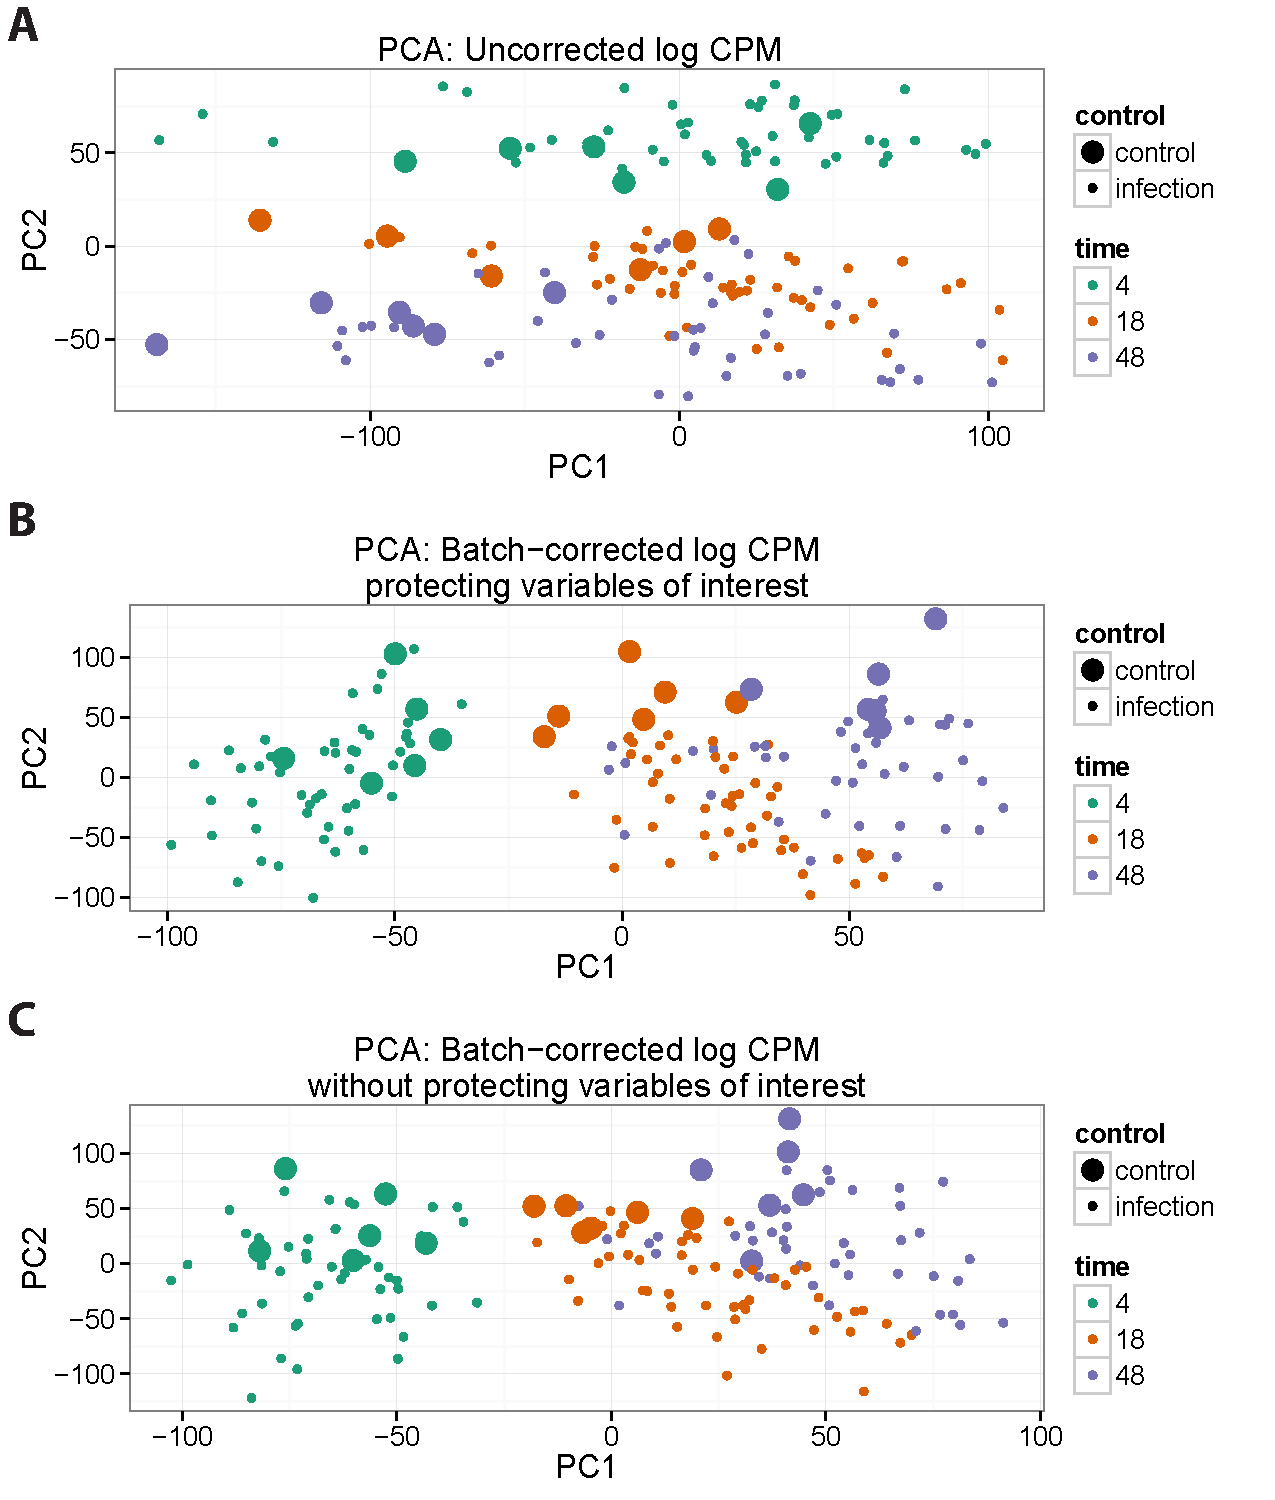
\includegraphics[width=5in]{img/ch02/fig-S02-pca.pdf}
\caption[Principal components analysis (PCA) of uncorrected and
  batch-corrected expression values.]{\textbf{Principal components
    analysis (PCA) of uncorrected and batch-corrected expression
    values.} (A) PCA of the TMM-normalized
  log\textsubscript{2}-transformed counts per million (CPM). Infected
  and control samples are not well separated.  PC2 separates the
  samples by timepoint. (B) PCA of the TMM-normalized
  log\textsubscript{2}-transformed CPM after removing the effects of
  RIN score and processing batch. PC1 separates the samples by
  timepoint. PC2 separates the infected and control samples. (C) PCA
  of the TMM-normalized log\textsubscript{2}-transformed CPM after
  removing the effects of RIN score and processing batch without
  protecting the variables of interest (individual, bacteria,
  timepoint).}
\label{fig:pca}
\end{figure}

\begin{figure}[!htb]
\centering
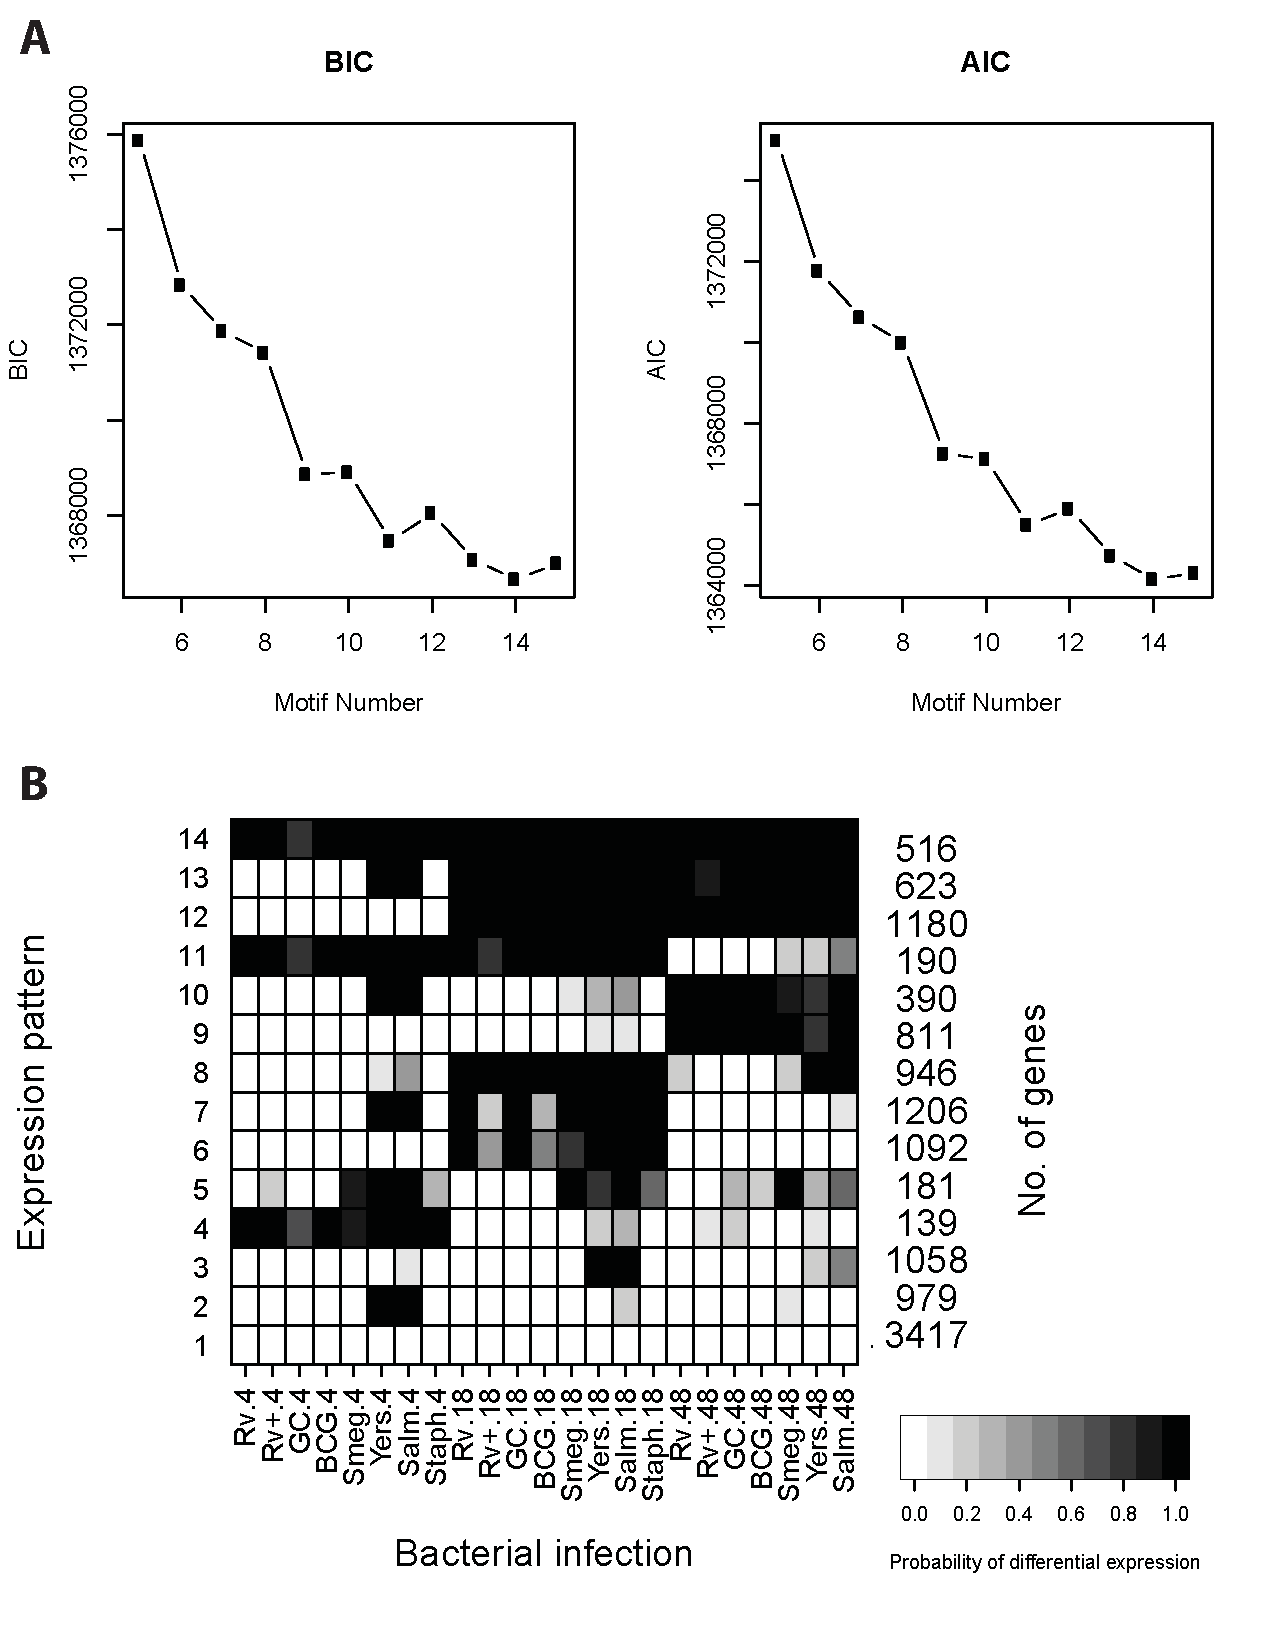
\includegraphics[width=5in]{img/ch02/fig-S03-joint-all-k14.pdf}
\caption[Joint Bayesian analysis with 14 expression
  patterns.]{\textbf{Joint Bayesian analysis with 14 expression
    patterns.} (A) Cormotif \citep{Wei2015} estimates the number of
  expression patterns (i.e.~motifs, using their terminology) to use by
  calculating the Bayesian information criterion (BIC) and the Akaike
  information criterion (AIC). These criteria penalize models for
  additional parameters to avoid overfitting. The model with the
  lowest BIC/AIC is considered the best fit, which in this context is
  the model with 14 expression patterns. (B) Joint analysis with
  Cormotif. The shading of each box represents the posterior
  probability that a gene assigned to the expression pattern (row) is
  differentially expressed in response to infection with a particular
  bacteria (column), with black representing a high posterior
  probability and white a low posterior probability.}
\label{fig:joint-all-k14}
\end{figure}

% Continues caption on next page. Requires package ccaption.
\begin{figure}[!htb]
  \contcaption{(continued) The expression patterns have the following
    interpretations: ``non-DE'' - Genes that do not respond to
    infection; ``Yers-Salm-4h'' - Genes that respond 4 hours
    post-infection with \emph{Y. pseudotuberculosis} or
    \emph{S. typhimurium}; ``Yers-Salm-18h'' - Genes that respond 18
    hours post-infection with \emph{Y. pseudotuberculosis} or
    \emph{S. typhimurium}; ``4h'' - Genes that respond to 4 hours
    post-infection with any bacteria; ``non-MTB'' - Genes that respond
    at 4, 18, and 48 hours post-infection to bacteria that are not MTB
    or BCG (attenuated \emph{M. bovis}); ``Virulent-18h'' - Genes that
    respond 18 hours post-infection with virulent bacteria;
    ``Virulent-18h+Yers-Salm-4h'' - Genes that respond 18 hours
    post-infection with virulent bacteria and 4 hours post-infection
    with \emph{Y. pseudotuberculosis} or \emph{S. typhimurium};
    ``18h+Yers-Salm-48h'' - Genes that respond 18 hours post-infection
    with any bacteria and 48 hours post-infection with \emph{Y.
      pseudotuberculosis} or \emph{S. typhimurium}; ``48h'' - Genes
    that respond 48 hours post-infection with any bacteria;
    ``48h+Yers-Salm-4h'' - Genes that respond 48 hours post-infection
    with any bacteria and 4 hours post-infection with \emph{Y.
      pseudotuberculosis} or \emph{S. typhimurium}; ``4\&18h'' - Genes
    that respond 4 and 18 hours post-infection with any bacteria;
    ``18\&48h'' - Genes that respond 18 and 48 hours post-infection
    with any bacteria; ``18\&48h+Yers-Salm-4h'' - Genes that respond
    18 and 48 hours post-infection with any bacteria and 4 hours
    post-infection with \emph{Y. pseudotuberculosis} or
    \emph{S. typhimurium}; ``All'' - Genes that respond at 4, 18, and
    48 hours post-infection with any bacteria.}
\end{figure}

\begin{figure}[!htb]
\centering \includegraphics[width=5in]{img/ch02/fig-S04-phago.pdf}
\caption[Expression of genes involved in phagosome
  maturation.]{\textbf{Expression of genes involved in phagosome
    maturation.} \emph{RAB22A}, \emph{RAP2A}, and \emph{ATP6V1D} are
  upregulated in response to infection with mycobacteria at 18 hours;
  whereas, \emph{RAB3A} and \emph{RAB33A} are downregulated (pattern
  ``MTB'' in Fig. \ref{fig:joint-18h}).}
\label{fig:phago}
\end{figure}

\begin{figure}[!htb]
\centering 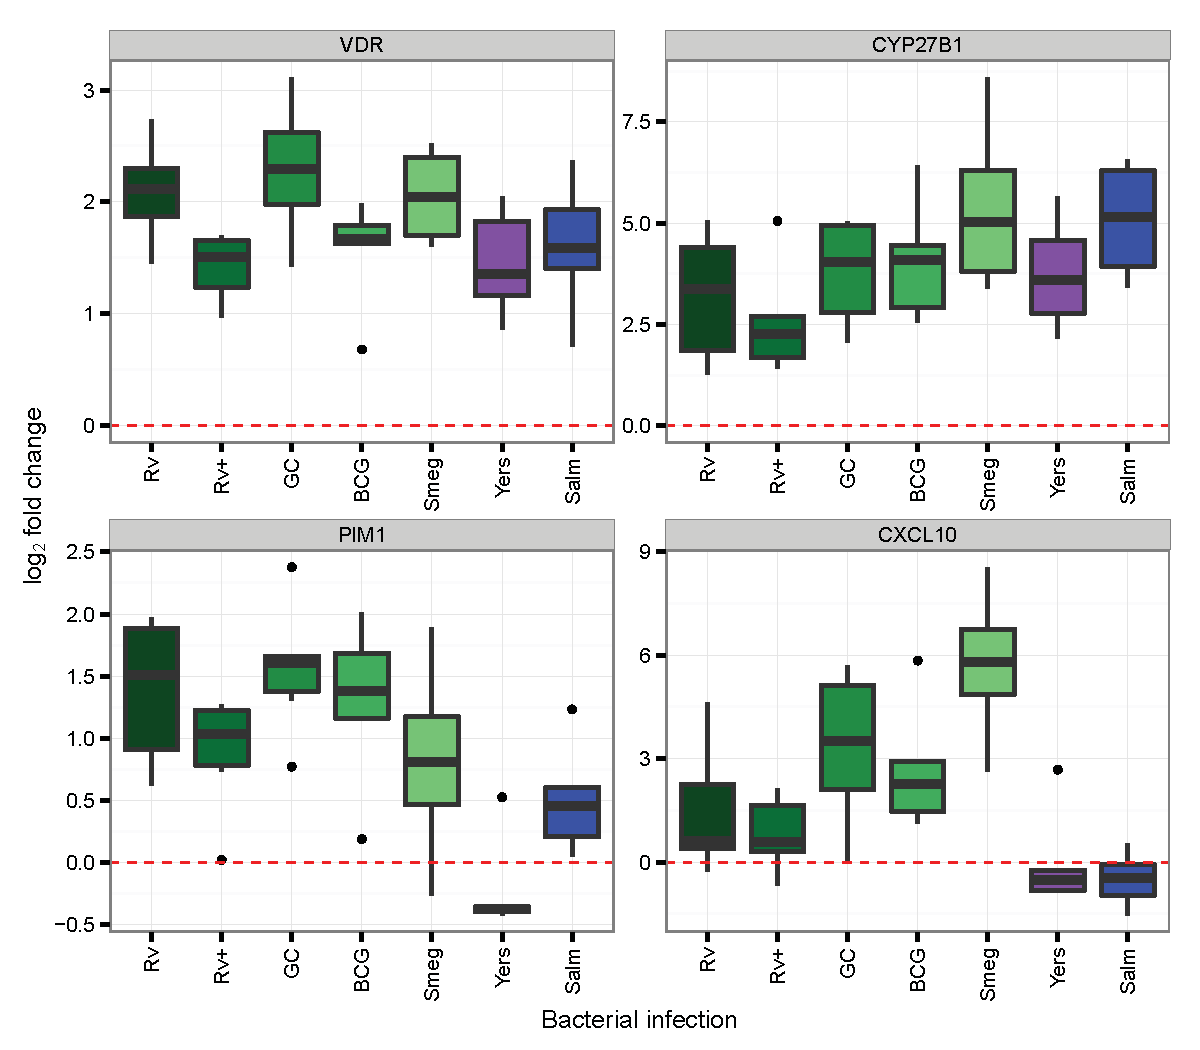
\includegraphics[width=5in]{img/ch02/fig-S05-vitD.pdf}
\caption[Expression of genes involved in vitamin D
  signaling.]{\textbf{Expression of genes involved in vitamin D
    signaling.}  \emph{VDR} and \emph{CYP27B1} are upregulated at 48
  hours post-infection with all bacteria (pattern ``All'' in Fig.
  \ref{fig:joint-48h}). \emph{PIM1} and \emph{CXCL10} are upregulated
  at 48 hours post-infection with the mycobacteria (pattern ``MTB'' in
  Fig. \ref{fig:joint-48h}).}
\label{fig:vitD}
\end{figure}

\begin{figure}[!htb]
\centering \includegraphics[width=5in]{img/ch02/fig-S06-dusp14.pdf}
\caption[Expression of \emph{DUSP14} at 18 hours
  post-infection.]{\textbf{Expression of \emph{DUSP14} at 18 hours
    post-infection.} \emph{DUSP14} is an example of an interesting
  gene not identified with our approach. At 18 hours, it is
  upregulated after infection with MTB H37Rv (q-value: 16\%), MTB
  GC1237 (q-value: 3\%), and BCG (q-value: 9\%) (the change in
  heat-inactivated MTB H37Rv had a q-value of 26\%); and downregulated
  post-infection with \emph{S. typhimurium} (q-value: 9\%).  Because
  it did not fit well into one of the main patterns of gene expression
  identified at 18 hours post-infection, it was classified as the
  ``non-DE'' pattern.}
\label{fig:dusp14}
\end{figure}

\begin{figure}[!htb]
\centering \includegraphics[width=5in]{img/ch02/fig-S07-Rv-v-GC.pdf}
\caption[Little difference in transcriptional response to infections
  with different MTB strains.]{\textbf{Little difference in
    transcriptional response to infections with different MTB
    strains.} Few statistically significant differences were
  identified when explicitly testing gene expression levels
  post-infection with MTB H37Rv and MTB GC1237 at 4, 18, or 48 hours
  post-infection (top, middle, and bottom panels, respectively). The
  volcano plots (left) display the -log\textsubscript{10} transformed
  p-value versus the log\textsubscript{2} fold change in expression
  level. The MA plots (right) display the log\textsubscript{2} fold
  change in expression level versus the average expression level. Most
  of the genes are labeled black indicating that their FDR value is
  greater than 5\%. Two genes (labeled green) at 4 hours
  post-infection had a q-value \textless{} 0.05 and
  log\textsubscript{2} fold change greater than 0.5 (see Supplementary
  Table \ref{tab:ch02-s8}).}
\label{fig:Rv-v-GC}
\end{figure}

\begin{figure}[!htb]
\centering
\includegraphics[width=5in]{img/ch02/fig-S08-ex-cytokines.pdf}
\caption[Response of example cytokines to infection with different MTB
  strains.]{\textbf{Response of example cytokines to infection with
    different MTB strains.} The log\textsubscript{2} fold change in
  expression of the pro-inflammatory cytokines \emph{TNF} and
  \emph{IL6} and the anti-inflammatory cytokine \emph{IL10} is similar
  post-infection with MTB H37Rv or MTB GC1237. \emph{TNF} and
  \emph{IL6} are upregulated at all three timepoints; whereas,
  \emph{IL10} is upregulated only at 4 hours post-infection.}
\label{fig:ex-cytokines}
\end{figure}

\begin{figure}[!htb]
\centering
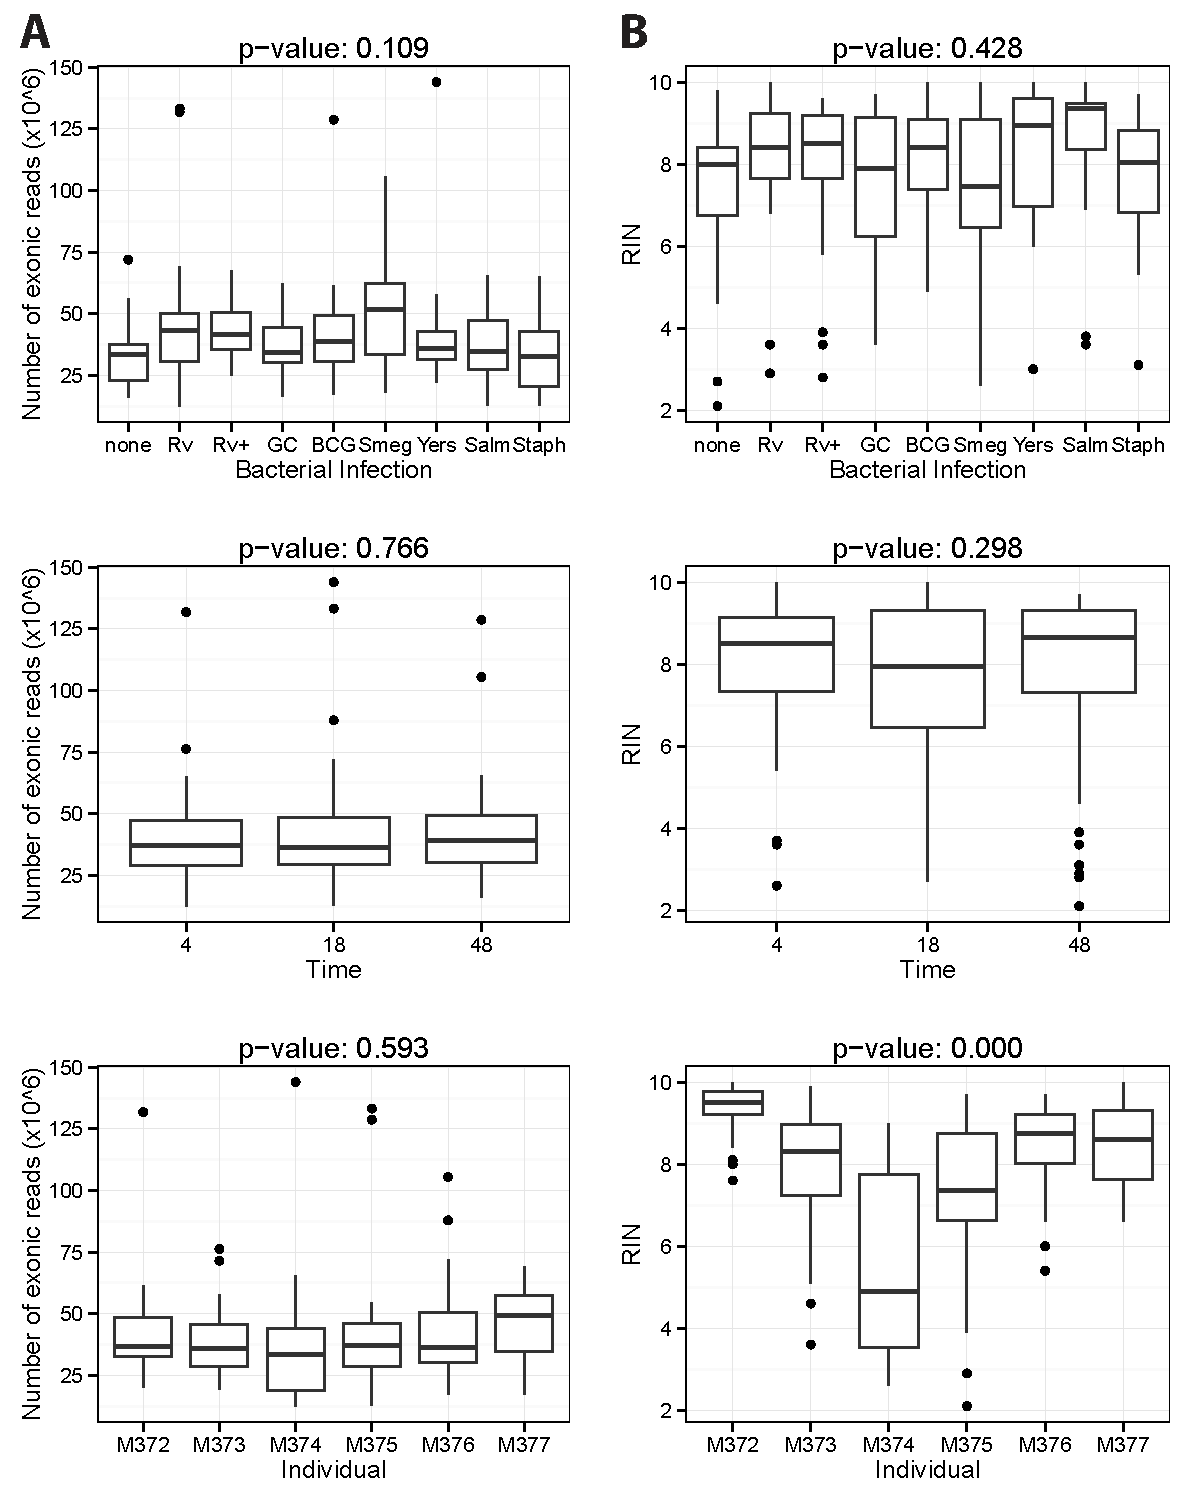
\includegraphics[width=5in]{img/ch02/fig-S09-rin-and-reads.pdf}
\caption[Distribution of the number of exonic reads and RNA quality
  scores (RIN) across variables of interest.]{\textbf{Distribution of
    the number of exonic reads and RNA quality scores (RIN) across
    variables of interest.} (A) The number of exonic reads is evenly
  distributed across the bacterial infections, timepoints, and
  individuals. (B) The RIN scores are evenly distributed across the
  bacterial infections and timepoints; however, the RIN does vary
  between the individuals.  The p-values are from an F-test.}
\label{fig:rin-and-reads}
\end{figure}

\begin{figure}[!htb]
\centering
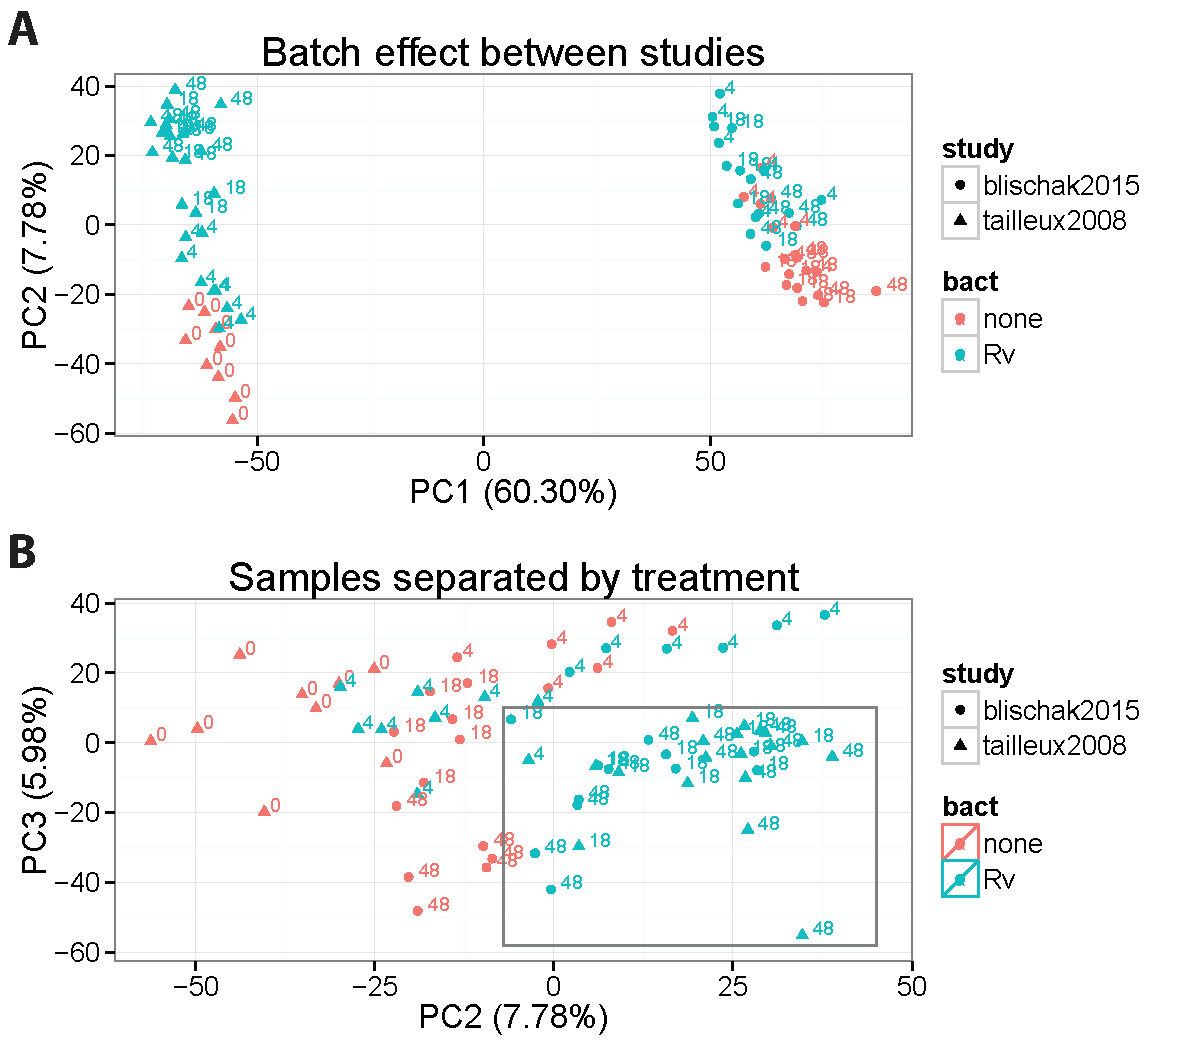
\includegraphics[width=5in]{img/ch02/fig-S10-tailleux2008.pdf}
\caption[Comparison to Tailleux et al., 2008.]{\textbf{Comparison to
    Tailleux et al., 2008.} We compared our RNA-seq data to the
  microarray data of Tailleux et al., 2008 \citep{Tailleux2008} to
  confirm a consistent signature of infection.  From our experiment,
  we used the batch-corrected TMM-normalized
  log\textsubscript{2}-transformed counts per million (CPM) from the
  MTB H37Rv infected macrophages at 4, 18, and 48 hours post-infection
  and their time-matched controls. From their experiment, we used the
  log\textsubscript{2}-transformed quantile-normalized data from the
  MTB H37Rv infected macrophages at 4, 18, and 48 hours post-infection
  as well as the zero timepoint non-infection control. In addition to
  the difference in technology, the macrophages were isolated via
  positive selection in our study and negative selection in
  theirs. Despite these differences, we still observe a common
  transcriptional signature of infection when performing principal
  components analysis (PCA). (A) PC1 is the expected batch effect
  between the two experiments. (B) Plotting PC2 versus PC3, the
  infected samples at 18 and 48 hours (when there is a strong
  transcriptional response; see
  Fig. \ref{fig:differential-expression}A) from the two different
  studies cluster together. The quantile-normalized data from Tailleux
  et al., 2008 \citep{Tailleux2008} is available at
  \url{https://bitbucket.org/jdblischak/tb-data}.}
\label{fig:tailleux2008}
\end{figure}

\clearpage
\subsection{Supplementary Tables}\label{ch02-supplementary-tables}

\begin{table}[!htb]
\caption[Gene expression matrix.]{\textbf{Gene expression matrix.}
  (see supplementary file associated with this dissertation) Contains
  the batch-corrected log\textsubscript{2} counts per million for the
  12,728 Ensembl genes analyzed in this study for each of the 156
  samples. The column names are in the format
  ``individual.infection.time''. It can also be downloaded from
  \url{http://giladlab.uchicago.edu} or
  \url{https://bitbucket.org/jdblischak/tb-data}.}
\label{tab:ch02-s1}
\end{table}

\begin{table}[!htb]
\caption[Differential expression results.]{\textbf{Differential
    expression results.} (see supplementary file associated with this
  dissertation) Contains the differential expression statistics from
  limma. This includes the log\textsubscript{2} fold change (logFC),
  average expression level (AveExpr), t-statistic (t), p-value
  (P.Value), q-value (adj.P.Val), and log-odds (B). The column names
  also contain the infection and timepoint for the given
  comparison. It can also be downloaded from
  \url{http://giladlab.uchicago.edu} or
  \url{https://bitbucket.org/jdblischak/tb-data}.}
\label{tab:ch02-s2}
\end{table}

\begin{table}[!htb]
\caption[Joint Bayesian analysis results.]{\textbf{Joint Bayesian
    analysis results.} (see supplementary file associated with this
  dissertation) Contains the assigned expression patterns for the
  12,728 Ensembl genes analyzed in this study for each of the three
  analyses in Fig. \ref{fig:joint-all}, \ref{fig:joint-18h}, and
  \ref{fig:joint-48h}. The columns ``full\_time\_course'',
  ``time\_18h'', and ``time\_48h'' correspond to Fig.
  \ref{fig:joint-all}, \ref{fig:joint-18h}, and \ref{fig:joint-48h},
  respectively.}
\label{tab:ch02-s3}
\end{table}

\begin{table}[!htb]
\caption[Joint Bayesian analysis results with gene
  descriptions.]{\textbf{Joint Bayesian analysis results with gene
    descriptions.} (see supplementary file associated with this
  dissertation) Contains the assigned expression patterns for the
  12,728 Ensembl genes analyzed in this study for each of the three
  analyses in Fig. \ref{fig:joint-all}, \ref{fig:joint-18h}, and
  \ref{fig:joint-48h}. It is the same information as Supplementary
  Table \ref{tab:ch02-s3}, but with the genes from each pattern from
  each of the three figures in its own sheet of the
  workbook. Furthermore, it contains the gene descriptions from
  Ensembl.}
\label{tab:ch02-s4}
\end{table}

\begin{table}[!htb]
\caption[Gene ontology results.]{\textbf{Gene ontology results.} (see
  supplementary file associated with this dissertation) Contains the
  gene ontology results for each of the expression patterns for the
  three analyses in Fig. \ref{fig:joint-all}, \ref{fig:joint-18h}, and
  \ref{fig:joint-48h}.}
\label{tab:ch02-s5}
\end{table}

\begin{table}[!htb]
\caption[RNA quality.]{\textbf{RNA quality.} (see supplementary file
  associated with this dissertation) Contains the RNA Integrity Number
  (RIN) and molarity (nmol/L) measured with a Bioanalyzer (Agilent)
  for each of the 156 samples.}
\label{tab:ch02-s6}
\end{table}

\begin{table}[!htb]
\caption[Number of differentially expressed genes from intersecting
  gene lists.]{\textbf{Number of differentially expressed genes from
    intersecting gene lists.} (see supplementary file associated with
  this dissertation) Contains the results of intersecting lists of
  differentially expressed genes for all pairwise comparisons (within
  each of the three timepoints).}
\label{tab:ch02-s7}
\end{table}

\begin{table}[!htb]
\caption[Number of differentially expressed genes from pairwise
  tests.]{\textbf{Number of differentially expressed genes from
    pairwise tests.} (see supplementary file associated with this
  dissertation) Contains the number of differentially expressed genes
  when performing all pairwise tests between bacterial infections for
  each of the three timepoints.}
\label{tab:ch02-s8}
\end{table}

\begin{table}[!htb]
\caption[Concordance in direction of effect for genes in each
  expression pattern.]{\textbf{Concordance in direction of effect for
    genes in each expression pattern.} (see supplementary file
  associated with this dissertation) Cormotif does not distinguish
  between the direction of the effect when assigning a gene to a given
  expression pattern. For example, a gene that is upregulated in one
  infection but downregulated in another is indistinguishable from a
  gene that is upregulated in response to both infections. However, in
  this data set, this is a rare effect. We calculated the percent
  concordance for the genes in the expression patterns from the three
  separate analyses. For example, for the expression pattern ``MTB'',
  100\% would indicate the gene is regulated in the same direction in
  the five mycobacterial infections, 80\% would indicate that the gene
  is regulated in the same direction for four of the five
  mycobacterial infections, etc. ``num\_concord'' is the number of
  genes in that expression pattern that are 100\% concordant across
  the infections. ``num\_discord'' is the number of genes in that
  expression pattern that are not 100\%
  concordant. ``mean\_perc\_concord'' is the mean percent concordance
  of all the genes in that expression pattern.}
\label{tab:ch02-s9}
\end{table}


% Chapter 03
\chapter{Predicting susceptibility to tuberculosis based on gene expression profiling}\label{ch:tb-suscept}

\section[Abstract]{Abstract\footnotemark}

Tuberculosis is a deadly infectious disease, which kills millions of
people every year. The causative pathogen, \emph{Mycobacterium
  tuberculosis} (MTB), is estimated to have infected up to a third of
the world's population; however, only approximately 10\% of healthy
individuals progress to active TB disease. Despite evidence for
heritability, it is not currently possible to predict whether a
healthy person is susceptible to TB. To explore approaches to classify
susceptibility to TB, we infected dendritic cells (DCs) from
individuals known to be susceptible or resistant to TB with MTB, and
measured genome-wide gene expression levels in infected and uninfected
cells. We found hundreds of differentially expressed genes between
susceptible and resistant individuals in the non-infected cells. We
further found that genetic polymorphisms in proximity to the
differentially expressed genes between susceptible and resistant
individuals are more likely to be associated with TB susceptibility in
published GWAS data. In particular, we identified two promising
candidate genes: \emph{CCL1} and \emph{UNC13A}. Lastly, we trained a
classifier based on the gene expression levels in the non-infected
cells, and demonstrated decent performance on our data and an
independent data set. Overall, our promising results from this small
study suggest that training a classifier on a larger cohort may enable
us to accurately predict TB susceptibility.

\footnotetext{Citation for chapter: John D Blischak*, Ludovic
  Tailleux*, Marsha Myrthil, Luis B Barreiro, and Yoav
  Gilad. Predicting susceptibility to tuberculosis based on gene
  expression profiling. In preparation. * denotes equal contribution.}

\section{Introduction}\label{ch03-introduction}

Tuberculosis (TB) is a major public health issue. Worldwide, over a
million people die of TB annually, and millions more currently live
with the disease \citep{WHO2015a, WHO2015b, Glaziou2015}. Successful
treatment requires months of antibiotic therapy \citep{Sotgiu2015},
and the difficulty of adhering to the full treatment regimen has lead
to the emergence of drug-resistant strains of \emph{Mycobacterium
  tuberculosis} (MTB) \citep{Seung2015}.

Approximately a third of the world's population has been infected with
MTB, but most are asymptomatic. While these naturally resistant
individuals are able to avoid active disease, MTB persists in a
dormant state inside their innate immune cells, known as a latent TB
infection \citep{Munoz2015}. In contrast, approximately 10\% of
individuals will develop active TB after infection with MTB
\citep{North2004, OGarra2013}. Unfortunately, we are currently unable
to predict if an individual is susceptible. While twin and family
studies have indicated a heritable component of TB susceptibility
\citep{Kallmann1943, Comstock1978, Cobat2010, Moller2010}, genome wide
association studies (GWAS) have only identified a few loci with low
effect size \citep{Thye2010, Mahasirimongkol2012, Thye2012, Png2012,
  Chimusa2014, Curtis2015, Sobota2016}. Due to the highly polygenic
architecture, it may be informative to examine differences between
susceptible and resistant individuals at a higher level of
organization, e.g. gene regulatory networks. Using this approach,
previous studies have characterized gene expression profiles in innate
immune cells isolated from individuals known to be susceptible or
resistant to infectious diseases, including tuberculosis
\citep{Thuong2008} and acute rheumatic fever \citep{Bryant2014}.

We hypothesized that gene expression profiles in innate immune cells
may be used to classify individuals with respect to their
susceptibility to develop an active TB infection. To test this
hypothesis, we isolated innate immune cells from individuals that are
resistant or susceptible to TB and infected them with MTB. We
discovered that the gene expression differences between resistant and
susceptible innate immune cells were present primarily in the
non-infected state, that these differentially expressed genes were
enriched for nearby SNPs with low p-values in TB susceptibility GWAS,
and furthermore, that these gene expression levels could be used to
classify individuals based on their susceptibility status.

\section{Results}

\subsection{Susceptible individuals have an altered transcriptome in the non-infected state}

We obtained whole blood samples from 25 healthy individuals
(Supplementary Table \ref{ch03-s1}). Six of the donors had recovered
from a previous active TB infection, and are thus susceptible. The
remaining 19 tested positive for a latent TB infection without ever
experiencing symptoms of active TB, and are thus resistant. We
isolated dendritic cells (DCs) and treated them with
\emph{Mycobacterium }\emph{tuberculosis} (MTB) or a mock control for
18 hours. To measure genome-wide gene expression levels in infected
and non-infected samples, we isolated and sequenced RNA using a
processing pipeline designed to minimize the introduction of unwanted
technical variation (Supplementary Fig. \ref{fig:process}). We
obtained a mean ($\pm$ SEM) of 48 $\pm$ 6 million raw reads per
sample. We performed quality control analyses to remove non-expressed
genes (Supplementary Fig.  \ref{fig:gene}; Supplementary Table
\ref{ch03-s2}), identify and remove outliers (Supplementary
Fig. \ref{fig:heat-all}, \ref{fig:heat-filt}, \ref{fig:outliers}), and
check for confounding batch effects (Supplementary
Fig. \ref{fig:batch-effect}, \ref{fig:infection}). Ultimately 6
samples failed the quality checks and were removed from all downstream
analyses (Supplementary Fig. \ref{fig:outliers}).

We performed a standard differential expression analysis using a
linear modeling framework (Supplementary Table \ref{ch03-s3}), defined
in equation (\ref{eq:limma}). As expected, there was a strong response
to infection with MTB in both resistant and susceptible individuals
(Supplementary Fig. \ref{fig:limma-supp}). Considering the resistant
individuals, we identified 3,486 differentially expressed (DE) genes
between the non-infected and infected states at a q-value of 10\% and
an arbitrary absolute log-fold change greater than 1. Similarly, 3,789
genes were DE between the non-infected and infected states for
susceptible individuals at a q-value of 10\% and an absolute log fold
change greater than 1. The DE genes included the important immune
response factors \emph{IL12B}, \emph{REL}, and \emph{TNF}. While the
treatment effect was obvious in all individuals, of most interest were
the patterns of gene expression differences between susceptible and
resistant individuals in either the non-infected or infected states
(Fig. \ref{fig:limma}). We identified 645 DE genes between resistant
and susceptible individuals in the non-infected state at a q-value of
10\%, including \emph{ATPV1B2}, \emph{FEZ2}, \emph{PSMA2},
\emph{TNFRSF25}, and \emph{TRIM38}. In contrast, no genes were DE
between resistant and susceptible individuals in the infected state
(q-value of 10\%).

\begin{figure}
\centering \includegraphics[width=5in]{img/ch03/limma.pdf}
\caption[Differential expression analysis.]{ \textbf{Differential
    expression analysis.} The top panel contains the distribution of
  unadjusted p-values after testing for differential expression
  between susceptible and resistant individuals in the (a)
  non-infected or (b) infected state. The bottom panel contains the
  corresponding volcano plots for the (c) non-infected and (d)
  infected states. The x-axis is the log fold change in gene
  expression level between susceptible and resistant individuals and
  the y-axis is the –log\textsubscript{10} p-value. Red indicates
  genes which are significant differentially expressed with a q-value
  less than 10\%.  }
\label{fig:limma}
\end{figure}
\subsection{Differentially expressed genes are enriched with TB susceptibility loci}

We next sought evidence that genes classified as DE in our \emph{in
  vitro} experimental system play a role in determining susceptibility
to TB. To do this, we intersected our results with those from a TB
susceptibility GWAS conducted in The Gambia and Ghana
\citep{Thye2010}.  To perform a combined analysis of the both data
sets, we coupled each gene in our expression data with the GWAS SNP
with the lowest p-value among all tested SNPs located within 50 kb of
the gene's transcription start site (Supplementary Table
\ref{ch03-s4}). We then asked whether the GWAS SNPs coupled with the
genes we classified as DE between susceptible and resistant
individuals in our experiment are enriched for low GWAS p-values
compared to SNPs coupled to randomly chosen genes.  Specifically, we
calculated the fraction of SNPs with a GWAS p-value less than 0.05
among SNPs coupled with ranked subsets of genes whose expression
profiles show increasing difference between susceptible and resistant
individuals (the effect size was the absolute value of the log fold
change in our experiment). In order to assess the significance of the
observations, we performed 100 permutations of the enrichment analysis
to derive an empirical p-value (Fig.  \ref{fig:gwas}b). Using this
approach, we observed a clear enrichment (empirical \emph{P} \textless
\, 0.01) of low GWAS p-values for SNPs coupled with the genes
classified as DE between susceptible and resistant individuals
(Fig. \ref{fig:gwas}a). We obtained similar results for the Ghana
GWAS; see Supplementary Fig.  \ref{fig:gwas-supp}).

We used this combined expression and GWAS data set to identify genes
potentially involved in TB susceptibility. Only two genes, \emph{CCL1}
and \emph{UNC13A}, were associated with a p-value less than 0.01 in
both The Gambia and Ghana GWAS and had an absolute log fold change
greater than 2 between susceptible and resistant individuals in the
non-infected state (these arbitrary cutoffs were chosen to be
stringent; see Supplementary Table \ref{ch03-s4} for the results with
various cutoffs). Interestingly, these two genes were previously shown
to play a role in MTB infection.

\begin{figure}
\centering \includegraphics[width=5in]{img/ch03/gwas.pdf}
\caption[Comparison of differential expression and The Gambia GWAS
  results.]{ \textbf{Comparison of differential expression and The
    Gambia GWAS results.} (a) The y-axis is the fold enrichment
  (y-axis) of genes assigned a SNP with p-value less than 0.05 from
  the GWAS in The Gambia \citep{Thye2010}. The x-axis is bins of genes
  with increasingly stringent effect size cutoffs of the absolute log
  fold change between susceptible and resistant individuals in the
  non-infected state. The effect size cutoffs were chosen such that
  each bin from left to right contained approximately 25 fewer
  genes. The red line is the results from the actual data. The grey
  lines are the results from 100 permutations. The dashed blue line at
  y=1 is the null expectation. (b) The x-axis is each of the 4
  differential expression tests performed.  The y-axis is the area
  under the curve of the fold enrichment. The boxplot is the result of
  the 100 permutations, and the red point is the result from the
  actual data. As a reference, the leftmost boxplot corresponds to the
  enrichment plot in (a).  }
\label{fig:gwas}
\end{figure}

\subsection{Susceptibility status can be predicted based on gene expression data}

Next we attempted to build a gene expression-based classifier to
predict TB susceptibility status (Supplementary Table
\ref{ch03-s5}). We focused on the gene expression levels measured in
the non-infected state both because this is where we observed the
largest gene regulatory differences between susceptible and resistant
individuals (Fig.  \ref{fig:limma}ac), and also because, from the
perspective of a translational application, it is more practical to
obtain gene expression data from non-infected DCs. We trained a
support vector machine using the 99 genes that were differentially
expressed between resistant and susceptible individuals in the
non-infected state at a q-value less than 5\% (see Methods for a full
description of how we selected this model). Encouragingly, we observed
a clear separation between susceptible and resistant individuals when
comparing the predicted probability of being resistant to TB for each
sample obtained from leave-one-out-cross-validation (Fig.
\ref{fig:classifier}a). Using a cutoff of 0.75 for the predicted
probability of being resistant to TB, we obtained a sensitivity of
100\% (5 out of 5 susceptible individuals classified as susceptible)
and a specificity of \mytilde88\% (15 out of 17 resistant individuals
were classified as resistant).

Unfortunately our current data set is too small to properly split into
separate training and testing sets (it is challenging to collect
samples from previous TB patients, who are healthy and have no medical
reason to go back for a GP visit). To our knowledge, there are also no
other similar data sets available. Thus, in order to further assess
the plausibility of our model, we applied the classifier to an
independent study, which collected genome-wide gene expression levels
in DCs from 65 healthy individuals \citep{Barreiro2012}, none with a
previous history of TB. Using the cutoff of 0.75 for the probability
of being resistant to TB (determined to be optimal in the training
set), \mytilde11\% (7 of 65) of the individuals were classified as
susceptible to TB. This result is intriguing similar to the estimate
that roughly 10\% of the general population is susceptible to TB
(Fig. \ref{fig:classifier}b).

\begin{figure}
\centering \includegraphics[width=5in]{img/ch03/classifier-svm.pdf}
\caption[Classifying TB susceptible individuals using a support vector
  machine model.]{ \textbf{Classifying TB susceptible individuals
    using a support vector machine model.} (a) The estimates of
  predicted probability of TB resistance from the
  leave-one-out-cross-validation for individuals in the current
  study. The blue circles represent individuals known to be
  susceptible to TB, and orange those resistant to TB. The horizontal
  dashed red line at a probability of 0.75 separates susceptible and
  resistant individuals. (b) The estimates of predicted probability of
  TB resistance from applying the classifier trained on the data from
  the current study to a test set of independently collected healthy
  individuals \citep{Barreiro2012}.  }
\label{fig:classifier}
\end{figure}

\section{Discussion}

We obtained dendritic cells (DCs) from individuals that were known to
be susceptible or resistant to developing active tuberculosis (TB) and
measured genome-wide gene expression levels in non-infected DCs and
DCs infected with \emph{Mycobacterium tuberculosis} (MTB) for 18
hours. As expected, there were large changes in gene expression due to
MTB infection in both resistant and susceptible individuals
(Supplementary Fig. \ref{fig:limma-supp}). We identified 645 genes,
which were differentially expressed (DE) between susceptible and
resistant individuals in the non-infected state; whereas, we did not
observe any DE genes between susceptible and resistant individuals in
the infected state (Fig. \ref{fig:limma}). This suggests that the
differences in the transcriptomes between DCs of resistant and
susceptible individuals are present pre-infection, and affect the
initial response to MTB. Yet, 18 hours after infection gene expression
profiles in both susceptible and resistant individuals have converged
to the same gene regulatory network to fight the active infection. We
chose to measure gene expression 18 hours post-infection because this
time point was previously associated with a large change in
genome-wide gene expression levels \citep{Tailleux2008}. Given our
observations, however, future studies investigating the difference in
the innate immune response between individuals resistant and
susceptible to TB may want to focus on earlier time points post
infection.

Among the 645 DE genes between resistant and susceptible individuals
in the non-infected state, there were many interesting genes involved
in important innate immune activities critical for fighting MTB and
other pathogens such as autophagy \citep{Deretic2014,
  Castrejon-Jimenez2015}, phagolysosomal acidification, and antigen
processing. In particular, \emph{FEZ2}, a suppressor of autophagosome
formation \citep{Spang2014}, was down-regulated when DCs were infected
with MTB; however, in the non-infected DCs, this gene has elevated
expression level in susceptible compared with resistant individuals.
In turn, \emph{ATP6V1B2}, a gene coding for a subunit of the proton
transporter responsible for acidifying phagolysosomes
\citep{Sturgill-Koszycki1994, Hornef2002, Hestvik2005}, has increased
expression in susceptible individuals compared to resistant in the
non-infected state. Lastly, genes coding for nine subunits of the
proteasome, which is critical for processing of MTB antigens to be
presented via major histocompatibility complex (MHC) class I molecules
\citep{Flynn1992, Grotzke2009, Grotzke2010, LindestamArlehamn2014},
have increased expression in susceptible individuals compared to
resistant in the non-infected state. These genes are candidates for
future functional studies investigating the mechanisms of TB
susceptibility.

To our knowledge, our study was only the second to collect data from
\emph{in vitro} MTB infected innate immune cells isolated from
individuals known to be susceptible to MTB (Thuong et al., 2008).
However, there were substantial differences between our study and that
of Thuong et al., 2008 \citep{Thuong2008}. First, they isolated and
infected macrophages, the primary target host cell in which MTB
resides; whereas, we infected DCs, which play a larger role in
stimulating the adaptive immune response to MTB. Second, the
susceptible individuals in Thuong et al., 2008 had an active TB
infection at the time the cells were isolated; whereas, our
individuals had recovered from a past TB infection. Third, we
collected samples from a larger number of resistant individuals (19
versus 4), increasing our power to distinguish between the gene
expression profiles of susceptible and resistant individuals.

We observed that DE genes in our \emph{in vitro} experimental system
were enriched for lower GWAS p-values (Fig. \ref{fig:gwas}). This
suggests that such \emph{in vitro} approaches are informative for
interrogating the genetic basis of disease susceptibility. That being
said, we recognized multiple caveats with this analysis. First,
assigning SNPs to their nearest gene on the linear chromosome is
problematic because regulatory variants can have longer range effects.
Second, the fold enrichments we calculated, albeit statistically
significant, were modest, indicating there were also many SNPs with
low p-values nearby genes with low effect sizes in our experiment. It
is possible that these variants contribute to TB susceptibility by
affecting gene expression in other cell types or environmental
conditions. Third, the individuals in our study were Europeans;
whereas, the GWAS were conducted in Africans. Nevertheless,
considering these limitations, it was encouraging that we were able to
detect evidence of the genetic basis of TB susceptibility in this
system.

Not only did this analysis identify a global enrichment of TB
susceptibility loci, but by intersecting the expression and GWAS data,
we were able to identify two genes (\emph{CCL1} and \emph{UNC13A})
which were marginally significant in both. Interestingly, both of
these genes were previously shown to play important roles in MTB
infection. \emph{CCL1} is a chemokine that stimulates migration of
monocytes \citep{Miller1992}. In our study, it was upregulated in
susceptible individuals compared to resistant in both the non-infected
and infected states (but did not reach statistical significance in
either) and was statistically significantly upregulated with MTB
treatment. The previous differential expression study of TB
susceptibility mentioned above found that \emph{CCL1} was upregulated
to a greater extent 4 hours post MTB-infection in macrophages isolated
from individuals with an active TB infection (i.e. susceptible)
compared to individuals with a latent TB infection (i.e. resistant)
\citep{Thuong2008}. Additionally they performed a candidate gene
association study and found that SNPs nearby \emph{CCL1} were
associated with TB susceptibility. In a previous study from our lab,
we discovered that \emph{CCL1} was one of only 288 genes that were
differentially expressed in macrophages 48 hours post-infection with
MTB and related mycobacterial species but not unrelated virulent
bacteria \citep{Blischak2015}. \emph{UNC13A} is involved in vesicle
formation \citep{Sudhof2004}. In our study, it was downregulated in
susceptible individuals compared to resistant in both the non-infected
and infected states (but did not reach statistical significance in
either) and was statistically significantly upregulated with MTB
treatment. In our past study mapping expression quantitative trait
loci (eQTLs) in DCs 18 hours post-infection with MTB, \emph{UNC13A}
was one of only 98 genes which was associated with an eQTL
post-infection but not pre-infection, which we called an MTB-specific
eQTL \citep{Barreiro2012}. Thus our new results increased the evidence
that \emph{CCL1} and \emph{UNC13A} play important roles in TB
susceptibility.

Previous attempts to use gene expression based classifiers in the
context of TB have focused on predicting the status of an infection
rather than the susceptibility status of an individual
\citep{Berry2010, OGarra2013, Blankley2014}. In other words, the goal
of most previous study was to detect individuals in an early stage of
an active TB infection when antibiotic intervention would be most
effective or to monitor the effectiveness of a treatment regimen
\citep{Maertzdorf2015}. In contrast, our goal was not to distinguish
between an active or latent infection, but instead to be able to
determine susceptibility status before individuals have an active TB
infection. Even with our small sample size, we were able to
successfully train a classier with high sensitivity and decent
specificity. Because such a classification of susceptibility status
could affect the decision of whether or not to take antibiotics to
treat a latent TB infection \citep{Munoz2015}, false negatives
(susceptible individuals mistakenly classified as resistant) would be
much more harmful than false positives (resistant individuals
mistakenly classified as susceptible), which is why we emphasized
sensitivity over specificity.

At this time, we are not aware of any other data set from healthy
individuals known to be sensitive to TB, with which we can further
test our classifier. When we applied our classifier to an independent
set of non-infected DCs isolated from healthy individuals of unknown
susceptibility status, our model predicted that \mytilde11\% of the
individuals were susceptible TB, which reassuringly is similar to the
average in the general population (10\%). Despite this success, our
results must be interpreted cautiously as a proof-of-principle due to
our very small sample size of only 5 susceptible individuals. That
said, our promising results in this small study suggest that
collecting blood samples from a larger cohort of susceptible
individuals would enable building a gene expression based classifier
able to confidently assess risk of TB susceptibility. By reducing the
number of resistant individuals receiving treatment for a latent TB
infection, we can eliminate the adverse health effects of a 6 month
regimen of antibiotics for these individuals and also reduce the
selective pressures on MTB to develop drug resistance.
\section{Methods}

\subsection{Ethics Statement}

We recruited 25 subjects to donate a blood sample for use in our
study. All methods were carried out in accordance with relevant
guidelines and regulations. The experimental protocols were approved
by the Institutional Review Boards of the University of Chicago
(10-504-B) and the Institut Pasteur (IRB00006966). All study
participants provided written informed consent.
\subsection{Sample collection}

We collected whole blood samples from healthy Caucasian male
individuals living in France. The putatively resistant individuals
tested positive for a latent TB infection in an interferon-$\gamma$
release assay, but had never developed active TB. The putatively
sensitive individuals had developed active TB in the past, but were
currently healthy.
\subsection{Isolation and infection of dendritic cells}

We performed these experiments as previously described
\citep{Barreiro2012}. Briefly, we isolated mononuclear cells from the
whole blood samples using Ficoll-Paque centrifugation, extracted
monocytes via CD14 positive selection, and differentiated the
monocytes into dendritic cells (DCs) by culturing them for 5 days in
RPMI 1640 (Invitrogen) supplemented with 10\% heat-inactivated FCS
(Dutscher), L-glutamine (Invitrogen), GM-CSF (20 ng/mL; Immunotools),
and IL-4 (20 ng/mL; Immunotools). Next we infected the DCs with
\emph{Mycobacterium tuberculosis} (MTB) H37Rv at a multiplicity of
infection of 1-to-1 for 18 hours.
\subsection{RNA extraction and sequencing}

We extracted RNA using the Qiagen miRNeasy Kit and prepared sequencing
libraries using the Illumina TruSeq Kit. We sent the master mixes to
the University of Chicago Functional Genomics Facility to be sequenced
on an Illumina HiSeq 4000. We designed the batches for RNA extraction,
library preparation, and sequencing to balance the experimental
factors of interest and thus avoid potential technical confounders
(Supplementary Fig. \ref{fig:process}).
\subsection{Read mapping}

We mapped reads to human genome hg38 (GRCh38) using Subread
\citep{Liao2013} and discarded non-uniquely mapping reads. We
downloaded the exon coordinates of 19,800 Ensembl \citep{Yates2016}
protein-coding genes (Ensembl 83, Dec 2015, GRCh38.p5) using the
R/Bioconductor \citep{Huber2015} package biomaRt \citep{Durinck2005,
  Durinck2009} and assigned mapped reads to these genes using
featureCounts \citep{Liao2014}.
\subsection{Quality control}

First we filtered genes based on their expression level by removing
all genes with a transformed median log\textsubscript{2} counts per
million (cpm) of less than zero. This step resulted in a set of 11,336
genes for downstream analysis (Supplementary Fig. \ref{fig:gene},
Supplementary Table \ref{ch03-s2}). Next we used principal components
analysis (PCA) and hierarchical clustering to identify and remove 6
outlier samples (Supplementary Fig. \ref{fig:heat-all},
\ref{fig:heat-filt}, \ref{fig:outliers}). We did this systematically,
by removing any sample whose data projections did not fall within two
standard deviations of the mean for any of the first six PCs (for the
first PC, which separated the samples by treatment, we calculated a
separate mean for the non-infected and infected samples).

After filtering lowly expressed genes and removing outliers, we
performed the PCA again to check for any potential confounding
technical batch effects (Supplementary Fig. \ref{fig:batch-effect}).
Reassuringly, the major sources of variation in the data were from the
biological factors of interest. PC1 was strongly correlated with the
effect of treatment, and PCs 2-6 were correlated with inter-individual
variation. The only concerning technical factor was the infection
experiments, which were done in 12 separate batches (Supplementary
Fig. \ref{fig:process}). Infection batch correlated with PCs 3 and 5;
however, we verified that this variation was not confounded with our
primary outcome of interest, TB susceptibility (Supplementary Fig.
\ref{fig:infection}).
\subsection{Differential expression analysis}

We used limma+voom \citep{Smyth2004, Law2014, Ritchie2015} to
implement the following linear model to test for differential
expression:
\begin{equation} \label{eq:limma}
Y\ \sim \beta_{0} + X_{treat}\beta_{treat} + X_{status}\beta_{status}
+ X_{treat,status}\beta_{treat,status} + I + \epsilon
\end{equation}
where $\beta_{0}$ is the mean expression level in non-infected cells
of resistant individuals, $\beta_{treat}$ is the fixed effect of
treatment in resistant individuals, $\beta_{status}$ is the fixed
effect of susceptibility status in non-infected cells,
$\beta_{treat,status}$ is the fixed interaction effect of treatment in
susceptible individuals, and $I$ is the random effect of individual.
The random individual effect was implemented using the limma function
duplicateCorrelation \citep{Smyth2005}. To jointly model the data with
voom and duplicateCorrelation, we followed the recommended best
practice of running both voom and duplicateCorrelation twice in
succession \citep{Liu2015}.

We used the model to test different hypotheses (Supplementary Data
S3). We identified genes which were differentially expressed (DE)
between infected and non-infected DCs of resistant individuals by
testing $\beta_{treat} = 0$, genes which were DE between infected and
non-infected DCs of susceptible individuals by testing $\beta_{treat}
+ \beta_{treat,status} = 0$, genes which were DE between susceptible
and resistant individuals in the non-infected state by testing
$\beta_{status} = 0$, and genes which were DE between susceptible and
resistant individuals in the infected state by testing $\beta_{status}
+ \beta_{treat,status} = 0$. We corrected for multiple testing using
q-values estimated via adaptive shrinkage \citep{Stephens2016} and
considered differentially expressed genes as those with a q-value less
than 10\%.
\subsection{Combined analysis of gene expression data and GWAS results}

The GWAS p-values were from a study of TB susceptibility conducted in
The Gambia and Ghana \citep{Thye2010}. To perform a combined analysis
of the gene expression and GWAS data, we assigned each gene to the SNP
with the minimum GWAS p-value out of all the SNPs located within 50 kb
up or downstream of its transcription start site. Specifically, we
obtained the genomic coordinates of the SNPs with the R/Bioconductor
\citep{Huber2015} package SNPlocs.Hsapiens.dbSNP144.GRCh38 and matched
SNPs to nearby genes using GenomicRanges \citep{Lawrence2013}. 10,260
of the 11,336 genes were assigned an association p-value
(Supplementary Table \ref{ch03-s4}). For each of the 4 hypotheses we
tested, we performed an enrichment analysis. To do so, we calculated
the fraction of genes assigned a GWAS SNP with p-value less than 0.05
for bins of genes filtered by increasingly stringent cutoffs for the
observed differential expression effect size (the absolute value of
the log fold change) between susceptible and resistant
individuals. The effect size cutoffs were chosen such that on average
each subsequent bin differed by 25 genes. To measure enrichment, we
calculated the area under the curve using the R package flux
\citep{Jurasinski2014}. In order to assess significance, we calculated
the area under the curve for 100 permutations of the data. All
differential expression tests were statistically significantly
enriched for SNPs low GWAS p-values in both the The Gambia
(Fig. \ref{fig:gwas}b) and Ghana (Supplementary
Fig. \ref{fig:gwas-supp}) data sets.
\subsection{Classifier}

The training set included data from the 44 high-quality non-infected
samples from this study with known susceptibility status. The test set
included the 65 non-infected samples from one of our previous studies
in which the susceptibility status is unknown \citep{Barreiro2012},
and thus assumed to be similar to that in the general population
(\mytilde10\%). Because the two studies are substantially different,
we took multiple steps to make them comparable. First, we subset to
include only those 9,450 genes which were assayed in both.  Second,
because the dynamic range obtained from RNA-seq (current study) and
microarrays (previous study \citep{Barreiro2012}) were different, we
normalized the gene expression levels to a standard normal with $\mu =
0$ and $\sigma = 1$ (Supplementary Fig.
\ref{fig:combined-dist}). Third, we corrected for the large, expected
batch effect between the two studies by regressing out the first PC of
the combined expression data using the limma function
removeBatchEffect \citep{Ritchie2015} (Supplementary Fig.
\ref{fig:combined-pca}).

To identify genes to use in the classifier, we performed a
differential expression analysis on the normalized, batch-corrected
data from the current study using the same approach described above
(with the exception that we no longer used voom \citep{Law2014} since
the data were no longer counts). Specifically, we tested for
differential expression between susceptible and resistant individuals
in the non-infected state and identified sets of genes to use in the
classifier by varying the q-value cutoff. Cutoffs of 5\%, 10\%, 15\%,
20\%, and 25\% corresponded to gene set sizes of 99, 385, 947, 1,934,
and 3,697, respectively. We used the R package caret \citep{Kuhn2008}
to train 3 different machine learning models: elastic net
\citep{Friedman2010}, support vector machine \citep{Karatzoglou2004},
and random forest \citep{Liaw2002} (the parameters for each individual
model were selected using the Kappa statistic). To assess the results
of the model on the training data, we performed
leave-one-out-cross-validation (LOOCV). In order to choose the model
with the best performance, we calculated the difference between the
mean of the LOOCV-estimated probabilities of being TB resistant for
the samples known to be TB resistant and the corresponding mean for
the samples known to be TB susceptible. This metric emphasized the
ability to separate the susceptible and resistant individuals into two
separate groups. Using this metric, the best performing model was the
support vector machine with the 99 genes that are significantly
differentially expressed at a q-value of 5\% (Supplementary Fig.
\ref{fig:class-compare}, Supplementary Table \ref{ch03-s5}); however,
both the elastic net (Supplementary Fig. \ref{fig:class-en}) and
random forest (Supplementary Fig. \ref{fig:class-rf}) had similar
performance.  Lastly, we tested the classifier by predicting the
probability of being TB resistant in the 65 healthy samples (Fig.
\ref{fig:classifier}b). For evaluating the predictions on the test set
of individuals with unknown susceptibility status, we used a relaxed
cutoff of the probability of being TB resistant of 0.75, which was
based on the ability of the model at this cutoff to classify all TB
susceptible individuals in the training set as susceptible with only 2
false positives. As expected, the 99 genes used in the classifier had
similar normalized, batch-corrected median expression levels in the
non-infected state across both studies (Supplementary Fig.
\ref{fig:class-exp}).
\subsection{Software implementation}

We automated our analysis using Python (\url{https://www.python.org/})
and Snakemake \citep{Koster2012}. Our processing pipeline used the
general bioinformatics software FastQC
(\url{http://www.bioinformatics.babraham.ac.uk/projects/fastqc/}),
MultiQC \citep{Ewels2016}, samtools \citep{Li2009}, and bioawk
(\url{https://github.com/lh3/bioawk}). We used R \citep{R2015} for all
statistics and data visualization. We obtained gene annotation
information from the Ensembl \citep{Yates2016} and Lynx
\citep{Sulakhe2016} databases. The computational resources were
provided by the University of Chicago Research Computing Center. All
code is available for viewing and reuse at
\url{https://github.com/jdblischak/tb-suscept}.
\subsection{Data availability}

The raw fastq files will be deposited in NCBI's Gene Expression
Omnibus \citep{Edgar2002} before official publication.  The RNA-seq
gene counts and other summary data sets are included as Supplementary
Data and are also available for download at
\url{https://github.com/jdblischak/tb-suscept/data}.
\section{Acknowledgments}

We thank T. Thye for sharing the GWAS data with us. This study was
funded by National Institutes of Health (NIH) Grant AI087658 to YG and
LT. JDB was supported by NIH T32GM007197. The content is solely the
responsibility of the authors and does not necessarily represent the
official views of the NIH.
\section{Author Contributions}

YG, LT, and LBB conceived of the study and designed the experiments.
LT coordinated sample collection and performed the infection
experiments. MM extracted the RNA and prepared the sequencing
libraries. JDB analyzed the results. LBB and YG supervised the
project. JDB wrote the paper with input from all authors.

%\clearpage\newpage
\section{Supplementary Information}\label{ch03-supplementary-information}

\subsection{Supplementary Figures}

\begin{figure}[!htb]
\centering \includegraphics[width=5in]{img/ch03/processing.pdf}
\caption[Batch processing.]{ \textbf{Batch processing.} We designed
  the processing of the samples to minimize the introduction of
  technical batch effects. Specifically, we attempted to balance the
  processing of samples obtained from susceptible and resistant
  individuals. In the diagram, each box represents a
  batch. ``Infection'' labels the batches of the infection
  experiments, ``Arrival'' labels the batch shipments of cell lysates
  arrived in Chicago, USA from Paris, France, ``Extraction'' labels
  the batches of RNA extraction, ``Master Mix'' labels the batches of
  library preparation, and ``Sequencing'' labels the batches of flow
  cells. Each master mix listed in a flow cell batch was sequenced on
  only one lane of that flow cell.  }
\label{fig:process}
\end{figure}


\begin{figure}[!htb]
\centering
\includegraphics[width=5in]{img/ch03/gene-exp-distribution.pdf}
\caption[Gene expression distributions before and after filtering
  genes and samples.]{ \textbf{Gene expression distributions before
    and after filtering genes and samples.} The log\textsubscript{2}
  counts per million (cpm) of each sample is plotted as a dashed gray
  line. The solid red line represents the median value across all the
  samples. The vertical solid blue line at $x = 0$ represents the
  cutoff used to filter lowly expressed genes based on their median
  log\textsubscript{2} cpm. The left panel is the data from all 19,800
  genes and 50 samples, the middle panel is the data from the 11,336
  genes remaining after removing lowly expressed genes, and the right
  panel is the data from 11,336 genes and the 44 samples remaining
  after removing outliers.  }
\label{fig:gene}
\end{figure}

\begin{figure}[!htb]
\centering
\includegraphics[width=5in]{img/ch03/heatmap-all-samples.pdf}
\caption[Heatmap of correlation matrix of samples.]{ \textbf{Heatmap
    of correlation matrix of samples.} Each square represents the
  Pearson correlation between the log\textsubscript{2} cpm expression
  values of two samples. Red indicates a low correlation of zero and
  white represents a high correlation of 1. The dendrogram displays
  the results of hierarchical clustering with the complete linkage
  method.  The outliers of the non-infected samples are
  s04-suscept-noninf, r02-resist-noninf, and r06-resist-noninf. The
  outliers of the infected samples are s01-suscep-infect,
  r06-resist-infect, and r18-resist-infect.  }
\label{fig:heat-all}
\end{figure}

\begin{figure}[!htb]
\centering
\includegraphics[width=5in]{img/ch03/heatmap-no-outliers.pdf}
\caption[Heatmap of correlation matrix after removing outliers.]{
  \textbf{Heatmap of correlation matrix after removing outliers.} Each
  square represents the Pearson correlation between the
  log\textsubscript{2} cpm expression values of two samples. Red
  indicates a low correlation of zero and white represents a high
  correlation of 1. The dendrogram displays the results of
  hierarchical clustering with the complete linkage method.  }
\label{fig:heat-filt}
\end{figure}


\begin{figure}[!htb]
\centering \includegraphics[width=5in]{img/ch03/outliers.pdf}
\caption[Principal components analysis (PCA) to identify outliers.]{
  \textbf{Principal components analysis (PCA) to identify outliers.}
  PC1 versus PC2 (a), PC3 versus PC4 (b), and PC5 versus PC6 (c). Each
  sample is represented by its 3-letter ID. ``s'' stands for
  susceptible and ``r'' for resistant, and the text is colored on the
  basis of treatment status (purple is non-infected; green is
  infected). The value is parentheses in each axis is the percentage
  of total variation accounted for by that PC. The outliers are listed
  in (d). These samples do not fall within 2 standard deviations of
  the mean value of the PCs listed in the right column. Note that a
  separate mean was calculated for the non-infected and infected
  samples for PC1 only.  }
\label{fig:outliers}
\end{figure}


\begin{figure}[!htb]
\centering \includegraphics[width=5in]{img/ch03/batch-pca.pdf}
\caption[Check for technical batch effects using principal components
  analysis (PCA).]{ \textbf{Check for technical batch effects using
    principal components analysis (PCA).} (a) PC1 versus PC2. The text
  labels are the individual identifiers. Purple indicates non-infected
  samples and green indicates infected. (b) PC3 versus PC4. The colors
  indicate the different infection batches. (c) PC5 versus PC6. The
  colors indicate the different infection batches. (d) The Pearson
  correlation of PCs 1-6 with each of the recorded biological and
  technical covariates. The correlations vary from 0 (white) to 1
  (red).  }
\label{fig:batch-effect}
\end{figure}

\begin{figure}[!htb]
\centering \includegraphics[width=5in]{img/ch03/batch-infection.pdf}
\caption[Check for confounding effect of infection batch.]{
  \textbf{Check for confounding effect of infection batch.} PC3 (a)
  and PC5 (b) varied by the date of infection. Non-infected samples
  are in purple and infected samples in green. Importantly, however,
  this technical variation arising from infection batch did not
  correlate with the susceptibility status of the individuals (c and
  d). Resistant individuals are in orange and susceptible individuals
  in blue.  }
\label{fig:infection}
\end{figure}

\begin{figure}[!htb]
\centering \includegraphics[width=5in]{img/ch03/limma-supp.pdf}
\caption[Effect of treatment with MTB.]{ \textbf{Effect of treatment
    with MTB.} The top panel contains the distribution of unadjusted
  p-values after testing for differential expression between the
  non-infected and infected states in (a) resistant and (b)
  susceptible individuals. The bottom panel contains the corresponding
  volcano plots for the (c) resistant and (d) susceptible individuals.
  The x-axis is the log fold change in gene expression level between
  susceptible and resistant individuals and the y-axis is the
  –log\textsubscript{10} p-value. Red indicates genes which are
  significant differentially expressed with a q-value less than 10\%.
  Because of the extremely skewed p-value distribution, all genes are
  significantly differentially expressed at this false discovery rate.
}
\label{fig:limma-supp}
\end{figure}

\begin{figure}[!htb]
\centering \includegraphics[width=5in]{img/ch03/gwas-supp.pdf}
\caption[Comparison of differential expression and Ghana GWAS
  results.]{ \textbf{Comparison of differential expression and Ghana
    GWAS results.} (a) The y-axis is the fold enrichment (y-axis) of
  genes assigned a SNP with p-value less than 0.05 from the GWAS in
  Ghana \citep{Thye2010}. The x-axis is bins of genes with
  increasingly stringent effect size cutoffs of the absolute log fold
  change between susceptible and resistant individuals in the
  non-infected state. The effect size cutoffs were chosen such that
  each bin from left to right contained approximately 25 fewer
  genes. The red line is the results from the actual data. The grey
  lines are the results from 100 permutations. The dashed blue line at
  y=1 is the null expectation. (b) The x-axis is each of the 4
  differential expression tests performed. The y-axis is the area
  under the curve of the fold enrichment. The boxplot is the result of
  the 100 permutations, and the red point is the result from the
  actual data. As a reference, the leftmost boxplot corresponds to the
  enrichment plot in (a).  }
\label{fig:gwas-supp}
\end{figure}

\begin{figure}[!htb]
\centering
\includegraphics[width=5in]{img/ch03/combined-distributions.pdf}
\caption[Normalizing gene expression distributions.]{
  \textbf{Normalizing gene expression distributions.} (left) The
  distribution of the median log2 cpm of the RNA-seq data from the
  current study in red compared to the distribution of the median gene
  expression levels of the microarray data from Barreiro et al., 2012
  \citep{Barreiro2012} in blue. (right) The distributions of the same
  data sets after normalizing each sample to a standard normal
  distribution.  }
\label{fig:combined-dist}
\end{figure}

\begin{figure}[!htb]
\centering \includegraphics[width=5in]{img/ch03/combined-pca.pdf}
\caption[Principal components analysis (PCA) of combined data sets.]{
  \textbf{Principal components analysis (PCA) of combined data sets.}
  (a) PC1 versus PC2 of the combined data set of the RNA-seq data from
  the current study (red) and the microarray data from Barreiro et
  al., 2012 \citep{Barreiro2012} (blue). The large circles are
  non-infected samples, and the small circles are infected
  samples. The value in parentheses is the percentage of the total
  variation accounted for by that PC. (b) The same data after
  regressing the original PC1 in (a).  }
\label{fig:combined-pca}
\end{figure}

\begin{figure}[!htb]
\centering
\includegraphics[width=5in]{img/ch03/classifier-compare.pdf}
\caption[Comparing the classification results of different methods and
  number of input genes.]{ \textbf{Comparing the classification
    results of different methods and number of input genes.} We
  compared 3 different machine learning methods (elastic net, support
  vector machine, random forest) and used 5 different sets of input
  genes. The input genes (x-axis) were obtained by varying the q-value
  cutoff for differential expression between susceptible and resistant
  individuals in the non-infected state from 5\% to 25\%. The
  evaluation metric (y-axis) was the difference of the mean assigned
  probability of being TB resistant between the known resistant and
  susceptible individuals in the current study.  }
\label{fig:class-compare}
\end{figure}

\begin{figure}[!htb]
\centering \includegraphics[width=5in]{img/ch03/classifier-en.pdf}
\caption[Classifying TB susceptible individuals using an elastic net
  model.]{ \textbf{Classifying TB susceptible individuals using an
    elastic net model.} (a) The estimates of predicted probability of
  TB resistance from the leave-one-out-cross-validation for
  individuals in the current study.  The blue circles represent
  individuals known to be susceptible to TB, and orange those
  resistant to TB. The horizontal blue line at a probability of 0.75
  almost separates susceptible and resistant individuals. (b) The
  estimates of predicted probability of TB resistance from applying
  the classifier trained on the data from the current study to a test
  set of independently collected healthy individuals
  \citep{Barreiro2012}.  }
\label{fig:class-en}
\end{figure}

\begin{figure}[!htb]
\centering \includegraphics[width=5in]{img/ch03/classifier-rf.pdf}
\caption[Classifying TB susceptible individuals using a random forest
  model.]{ \textbf{Classifying TB susceptible individuals using a
    random forest model.}  (a) The estimates of predicted probability
  of TB resistance from the leave-one-out-cross-validation for
  individuals in the current study.  The blue circles represent
  individuals known to be susceptible to TB, and orange those
  resistant to TB. The horizontal blue line at a probability of 0.75
  separates susceptible and resistant individuals.  (b) The estimates
  of predicted probability of TB resistance from applying the
  classifier trained on the data from the current study to a test set
  of independently collected healthy individuals \citep{Barreiro2012}.
}
\label{fig:class-rf}
\end{figure}

\begin{figure}[!htb]
\centering \includegraphics[width=5in]{img/ch03/classifier-exp.pdf}
\caption[Comparing gene expression between the two studies.]{
  \textbf{Comparing gene expression between the two studies.} After
  normalization and batch-correction, the median expression levels of
  the 99 genes used in the classifier were similar between the samples
  in the current study and those in Barreiro et al., 2012
  \citep{Barreiro2012}. The dashed red line is the 1:1 line.  }
\label{fig:class-exp}
\end{figure}

\clearpage
\subsection{Supplementary Data}

\begin{table}[!htb]
\caption[Sample information.]{\textbf{Sample information.}  (see
  supplementary file associated with this dissertation) Contains
  information on the 50 samples. Most variables describe the batch
  processing steps outlined in Supplementary
  Fig. \ref{fig:process}. ``id'' is a unique identifier for each
  sample, ``individual'' is the individual identifier (``s'' =
  susceptible, ``r'' = resistant), ``status'' is the susceptibility
  status, ``treatment'' is if the sample was infected or non-infected,
  ``infection'' is the date of the infection experiment (12 total),
  ``arrival'' is the identifier for the arrival batch (4 total),
  ``extraction'' is the batch for RNA extraction (5 total),
  ``master\_mix'' is the batch for library preparation (3 total),
  ``rin'' is the RNA Integrity Number from the Agilent Bioanalyzer,
  and ``outlier'' is a Boolean variable indicating if the sample was
  identified as an outlier (Supplementary Fig.  \ref{fig:outliers})
  and removed from the analysis. (txt) }
\label{ch03-s1}
\end{table}

\begin{table}[!htb]
\caption[Gene expression matrix.]{ \textbf{Gene expression matrix.}
  (see supplementary file associated with this dissertation) Contains
  the gene expression counts for the 11,336 genes after filtering
  lowly expressed genes for all 50 samples (Supplementary
  Fig. \ref{fig:gene}). Each row is a gene labeled with its Ensembl
  gene ID. Each column is a sample. Each sample is labeled according
  to the pattern ``x\#\#-status-treatment'', where x is ``r'' for
  resistant or ``s'' for susceptible, \#\# is the ID number, status is
  ``resist'' for resistant or ``suscep'' for susceptible, and
  treatment is ``noninf'' for non-infected or ``infect'' for
  infected. (txt) }
\label{ch03-s2}
\end{table}

\begin{table}[!htb]
\caption[Differential expression results.]{ \textbf{Differential
    expression results.}  (see supplementary file associated with this
  dissertation) Contains the results of the differential expression
  analysis with limma (Fig. \ref{fig:limma}). The workbook contains 4
  sheets corresponding to the 4 tests performed. ``status\_ni'' is the
  test between resistant and susceptible individuals in the
  non-infected state, ``status\_ii'' is the test between resistant and
  susceptible individuals in the infected state, ``treat\_resist'' is
  the test between the non-infected and infected states for resistant
  individuals, and ``treat\_suscep'' is the test between the
  non-infected and infected states for susceptible individuals. Each
  sheet has the same columns. ``id'' is the Ensembl gene ID, ``gene''
  is the gene name, ``logFC'' is the log fold change from limma,
  ``AveExpr'' is the average log expression from limma, ``t'' is the
  t-statistic from limma, ``P.Value'' is the p-value from limma,
  ``adj.P.Val'' is the adjusted p-value from limma, ``qvalue'' is the
  q-value calculated with adaptive shrinkage, ``chr'' is the
  chromosome where the gene is located, ``description'' is the
  description of the gene from Ensembl, ``phenotype'' is the
  associated phenotype(s) assigned my Ensembl, ``go\_id'' is the
  associated GO term(s) assigned by Ensembl, and ``go\_description''
  is the corresponding name(s) of the GO term(s). (xlsx) }
\label{ch03-s3}
\end{table}

\begin{table}[!htb]
\caption[Data for combined analysis of gene expression data and GWAS
  results.]{ \textbf{Data for combined analysis of gene expression
    data and GWAS results.}  (see supplementary file associated with
  this dissertation) Contains the results of the GWAS comparison
  analysis (Fig. \ref{fig:gwas}). The first sheet ``input-data''
  contains the data for the 10,260 genes which were assigned a SNP in
  the studies from The Gambia and Ghana. ``gwas\_p\_ghana'' is the
  minimum p-value from the GWAS in Ghana, ``gwas\_p\_gambia'' is the
  minimum p-value from the GWAS in The Gambia, and ``n\_snps'' is the
  number of GWAS SNPs within 50 kb of the transcription start
  site. The columns status\_ni, status\_ii, treat\_resist, and
  treat\_suscep refer to the tests described for Supplementary Table
  \ref{ch03-s3} and contain the absolute log fold changes for each
  comparison. All the other gene annotation columns are the same as
  described for Supplementary Table \ref{ch03-s3}. The second sheet
  ``top-genes'' contains the results of stringently filtering the
  combined differential expression and GWAS results. ``GWAS P cutoff''
  is the p-value cutoff used for both the The Gambia and Ghana GWAS,
  ``Effect size cutoff'' is the cutoff of the absolute log fold change
  for the test between susceptible and resistant individuals in the
  non-infected state (Fig. \ref{fig:limma}a), ``Number of genes'' is
  the number of genes which satisfied these thresholds, and ``Names''
  is the corresponding official gene names (sorted
  alphabetically). (xlsx) }
\label{ch03-s4}
\end{table}

\begin{table}[!htb]
\caption[Classifier results.]{ \textbf{Classifier results.}  (see
  supplementary file associated with this dissertation) Contains the
  results of the classifier analysis.  Specifically it contains the
  results from the support vector machine using the genes with a
  qvalue less than 0.05 (Fig.  \ref{fig:classifier}). The sheet
  ``gene-list'' contains information about the genes used for the
  classifier (the columns are described in the section for
  Supplementary Table \ref{ch03-s3}). The sheet ``training-input''
  contains the input gene expression data for training the model. The
  sheet ``training-results'' contains the results of the
  leave-one-out-cross-validation when training the model on the
  samples from the current study.  The sheet ``testing-input''
  contains the input gene expression data for testing the model. The
  sheet ``testing-results'' contains the results from testing the
  model on the samples from Barreiro et al., 2012
  \citep{Barreiro2012}. The column ``prob\_tb\_resist'' is the
  probability of being resistant to TB assigned by the model. (xlsx) }
\label{ch03-s5}
\end{table}


% Chapter 04
\chapter{Batch effects and the effective design of single-cell gene expression studies}\label{ch:singleCellSeq}

\section[Abstract]{Abstract\footnotemark}

Single-cell RNA sequencing (scRNA-seq) can be used to characterize
variation in gene expression levels at high resolution. However, the
sources of experimental noise in scRNA-seq are not yet well
understood.  We investigated the technical variation associated with
sample processing using the single-cell Fluidigm C1 platform. To do
so, we processed three C1 replicates from three human induced
pluripotent stem cell (iPSC) lines. We added unique molecular
identifiers (UMIs) to all samples, to account for amplification
bias. We found that the major source of variation in the gene
expression data was driven by genotype, but we also observed
substantial variation between the technical replicates. We observed
that the conversion of reads to molecules using the UMIs was impacted
by both biological and technical variation, indicating that UMI counts
are not an unbiased estimator of gene expression levels. Based on our
results, we suggest a framework for effective scRNA-seq studies.

\footnotetext{Citation for chapter: Po-Yuan Tung*, John D Blischak*,
  Chiaowen Hsiao*, David A Knowles, Jonathan E Burnett, Jonathan K
  Pritchard, and Yoav Gilad. Batch effects and the effective design of
  single-cell gene expression studies. bioRxiv, page 062919, 2016.  *
  denotes equal contribution. Accepted with minor revisions in
  Scientific Reports.}

\section{Introduction}\label{ch04-introduction}

Single-cell genomic technologies can be used to study the regulation
of gene expression at unprecedented resolution \citep{Macaulay2014,
  Saliba2014}. Using single-cell gene expression data, we can begin to
effectively characterize and classify individual cell types and cell
states, develop a better understanding of gene regulatory threshold
effects in response to treatments or stress, and address a large
number of outstanding questions that pertain to the regulation of
noise and robustness of gene expression programs. Indeed, single cell
gene expression data have already been used to study and provide
unique insight into a wide range of research topics, including
differentiation and tissue development \citep{Macosko2015, Handel2016,
  Drissen2016}, the innate immune response \citep{Shalek2013,
  Jaitin2014}, and pharmacogenomics \citep{Miyamoto2015, Kim2015}.

Yet, there are a number of outstanding challenges that arose in
parallel with the application of single cell technology
\citep{Stegle2015}. A fundamental difficulty, for instance, is the
presence of inevitable technical variability introduced during sample
processing steps, including but not limited to the conditions of mRNA
capture from a single cell, amplification bias, sequencing depth, and
variation in pipetting accuracy. These (and other sources of error)
may not be unique to single cell technologies, but in the context of
studies where each sample corresponds to a single cell, and is thus
processed as a single unrepeatable batch, these technical
considerations make the analysis of biological variability across
single cells particularly challenging.

To better account for technical variability in scRNA-seq experiments,
it has become common to add spike-in RNA standards of known abundance
to the endogenous samples \citep{Brennecke2013, Grun2014}. The most
commonly used spike-in was developed by the External RNA Controls
Consortium (ERCC) \citep{Jiang2011}; comprising of a set of 96 RNA
controls of varying length and GC content. A number of single cell
studies focusing on analyzing technical variability based on ERCC
spike-in controls have been reported \citep{Brennecke2013, Grun2014,
  Ding2015, Vallejos2015}. However, one principle problem with
spike-ins is that they do not `experience' all processing steps that
the endogenous sample is subjected to. For that reason, it is unknown
to what extent the spike-ins can faithfully reflect the error that is
being accumulated during the entire sample processing procedure,
either within or across batches. In particular, amplification bias,
which is assumed to be gene-specific, cannot be addressed by spike-in
normalization approaches.

To address challenges related to the efficiency and uniformity with
which mRNA molecules are amplified and sequenced in single cells,
unique molecule identifiers (UMIs) were introduced to single cell
sample processing \citep{Kivioja2011, Fu2011, Casbon2011,
  Shiroguchi2012}.  The rationale is that by counting molecules rather
than the number of amplified sequencing reads, one can account for
biases related to amplification, and obtain more accurate estimates of
gene expression levels \citep{Jaitin2014, Islam2014, Grun2014}. It is
assumed that most sources of variation in single cell gene expression
studies can be accounted for by using the combination of UMIs and a
spike-in based standardization \citep{Islam2014,
  Vallejos2015}. Nevertheless, though molecule counts, as opposed to
sequencing read counts, are associated with substantially reduced
levels of technical variability, a non-negligible proportion of
experimental error remains unexplained.

There are a few common platforms in use for scRNA-seq. The automated
C1 microfluidic platform (Fluidigm), while more expensive per sample,
has been shown to confer several advantages over platforms that make
use of droplets to capture single cells \citep{Wu2014,
  Macosko2015}. In particular, smaller samples can be processed using
the C1 (when cell numbers are limiting), and the C1 capture efficiency
of genes (and RNA molecules) is markedly higher. Notably, in the
context of this study, the C1 system also allows for direct
confirmation of single cell capture events, in contrast to most other
microfluidic-based approaches \citep{Macosko2015, Klein2015}. One of
the biggest limitations of using the C1 system, however, is that
single cell capture and preparation from different conditions are
fully independent \citep{Hicks2015}.  Consequently, multiple
replicates of C1 collections from the same biological condition are
necessary to facilitate estimation of technical variability even with
the presence of ERCC spike-in controls \citep{Stegle2015}. To our
knowledge, to date, no study has been purposely conducted to assess
the technical variability across batches on the C1 platform.

To address this gap, we collected scRNA-seq data from induced
pluripotent stem cell (iPSC) lines of three Yoruba individuals
(abbreviation: YRI) using C1 microfluidic plates. Specifically, we
performed three independent C1 collections per each individual to
disentangle batch effects from the biological covariate of interest,
which, in this case, is the difference between individuals. Both ERCC
spike-in controls and UMIs were included in our sample
processing. With these data, we were able to elucidate technical
variability both within and between C1 batches and thus provide a deep
characterization of cell-to-cell variation in gene expression levels
across individuals.

\section{Results}\label{ch04-results}

\subsection{Study design and quality
control}\label{study-design-and-quality-control}

We collected single cell RNA-seq (scRNA-seq) data from three YRI iPSC
lines using the Fluidigm C1 microfluidic system followed by
sequencing.  We added ERCC spike-in controls to each sample, and used
5-bp random sequence UMIs to allow for the direct quantification of
mRNA molecule numbers. For each of the YRI lines, we performed three
independent C1 collections; each replicate was accompanied by
processing of a matching bulk sample using the same reagents. This
study design (Fig. \ref{fig:ch04-study-design}A and Supplementary
Table \ref{tab:ch04-s1}) allows us to estimate error and variability
associated with the technical processing of the samples, independently
from the biological variation across single cells of different
individuals. We were also able to estimate how well scRNA-seq data can
recapitulate the RNA-seq results from population bulk samples.

\begin{figure}
\centering \includegraphics[trim=0 .5in 0
  0,clip,width=5in]{img/ch04/Figure01.jpeg}
\caption[Experimental design and quality control of
  scRNA-seq.]{\textbf{Experimental design and quality control of
    scRNA-seq.} (A) Three C1 96 well-integrated fluidic circuit (IFC)
  replicates were collected from each of the three Yoruba
  individuals. A bulk sample was included in each batch. (B) Summary
  of the cutoffs used to remove data from low quality cells that might
  be ruptured or dead (See Supplementary Fig. \ref{fig:ch04-s1} for
  details). (C-E) To assess the quality of the scRNA-seq data, the
  capture efficiency of cells and the faithfulness of mRNA fraction
  amplification were determined based on the proportion of unmapped
  reads, the number of detected genes, the numbers of total mapped
  reads, and the proportion of ERCC spike-in reads across cells.  The
  dash lines indicate the cutoffs summarized in panel (B). The three
  colors represent the three individuals (NA19098 in red, NA19101 in
  green, and NA19239 in blue), and the numbers indicate the cell
  numbers observed in each capture site on C1 plate.}
\label{fig:ch04-study-design}
\end{figure}

% Continues caption on next page. Requires package ccaption.
\begin{figure}
\contcaption{(continued) (F) Scatterplots in log scale showing the
  mean read counts and the mean molecule counts of each endogenous
  gene (grey) and ERCC spike-ins (blue) from the 564 high quality
  single cell samples before removal of genes with low expression.
  (G) mRNA capture efficiency shown as observed molecule count versus
  number of molecules added to each sample, only including the 48 ERCC
  spike-in controls remaining after removal of genes with low
  abundance.  Each red dot represents the mean +/- SEM of an ERCC
  spike-in across the 564 high quality single cell samples.}
\end{figure}

In what follows, we describe data as originating from different
samples when we refer to data from distinct wells of each C1
collection.  Generally, each sample corresponds to a single cell. In
turn, we describe data as originating from different replicates when
we refer to all samples from a given C1 collection, and from different
individuals when we refer to data from all samples and replicates of a
given genetically distinct iPSC line.

We obtained an average of 6.3 +/- 2.1 million sequencing reads per
sample (range 0.4-11.2 million reads). We processed the sequencing
reads using a standard alignment approach (see Methods) and performed
multiple quality control analyses. As a first step, we estimated the
proportion of ERCC spike-in reads from each sample. We found that,
across samples, sequencing reads from practically all samples of the
second replicate of individual NA19098 included unusually high ERCC
content compared to all other samples and replicates (Supplementary
Fig. \ref{fig:ch04-s1}). We concluded that a pipetting error led to
excess ERCC content in this replicate and we excluded the data from
all samples of this replicate in subsequent analyses. With the
exception of the excluded samples, data from all other replicates seem
to have similar global properties (using general metrics;
Fig. \ref{fig:ch04-study-design}C-E and Supplementary
Fig. \ref{fig:ch04-s1}).

We next examined the assumption that data from each sample correspond
to data from a single cell. After the cell sorting was complete, but
before the processing of the samples, we performed visual inspection
of the C1 microfluidic plates. Based on that visual inspection, we
flagged 21 samples that did not contain any cell, and 54 samples that
contained more than one cell (across all batches). Visual inspection
of the C1 microfluidic plate is an important quality control step, but
it is not infallible. We therefore filtered data from the remaining
samples based on the number of total mapped reads, the percentage of
unmapped reads, the percentage of ERCC spike-in reads, and the number
of genes detected (Fig. \ref{fig:ch04-study-design}B-E). We chose
data-driven inclusion cutoffs for each metric, based on the 95th
percentile of the respective distributions for the 21 libraries that
were amplified from samples that did not include a cell based on
visual inspection (Supplementary Fig. \ref{fig:ch04-s1}). Using this
approach, we identified and removed data from 15 additional samples
that were classified as originating from a single cell based on visual
inspection, but whose data were more consistent with a multiple-cell
origin based on the number of total molecules, the concentration of
cDNA amplicons, and the read-to-molecule conversion efficiency
(defined as the number of total molecules divided by the number of
total reads; Supplementary Fig.  \ref{fig:ch04-s2}). At the conclusion
of these quality control analyses and exclusion steps, we retained
data from 564 high quality samples, which correspond, with reasonable
confidence, to 564 single cells, across eight replicates from three
individuals (Supplementary Table \ref{tab:ch04-s2}).

Our final quality check focused on the different properties of
sequencing read and molecule count data. We considered data from the
564 high quality samples and compared gene specific counts of
sequencing read and molecules. We found that while gene-specific reads
and molecule counts are exceptionally highly correlated when we
considered the ERCC spike-in data (r = 0.99;
Fig. \ref{fig:ch04-study-design}F), these counts are somewhat less
correlated when data from the endogenous genes are considered (r =
0.92). Moreover, the gene-specific read and molecule counts
correlation is noticeably lower for genes that are expressed at lower
levels (Fig.  1F). These observations concur with previous studies
\citep{Islam2014, Grun2014} as they underscore the importance of using
UMIs in single cell gene expression studies.

\begin{figure}
\centering \includegraphics[trim=0 .3in 0
  0,clip,width=5in]{img/ch04/Figure02.jpeg}
\caption[The effect of sequencing depth and cell number on single cell
  UMI estimates.]{\textbf{The effect of sequencing depth and cell
    number on single cell UMI estimates.} Sequencing reads from the
  entire data set were subsampled to the indicated sequencing depth
  and cell number, and subsequently converted to molecules using the
  UMIs. Each point represents the mean +/- SEM of 10 random draws of
  the indicated cell number. The left panel displays the results for
  6,097 (50\% of detected) genes with lower expression levels and the
  right panel the results for 6,097 genes with higher expression
  levels. (A) Pearson correlation of aggregated gene expression level
  estimates from single cells compared to the bulk sequencing
  samples. (B) Total number of genes detected with at least one
  molecule in at least one of the single cells.  (C) Pearson
  correlation of cell-to-cell gene expression variance estimates from
  subsets of single cells compared to the full single cell data set.}
\label{fig:subsample}
\end{figure}

We proceeded by investigating the effect of sequencing depth and the
number of single cells collected on multiple properties of the
data. To this end, we repeatedly subsampled single cells and
sequencing reads to assess the correlation of the single cell gene
expression estimates to the bulk samples, the number of genes
detected, and the correlation of the cell-to-cell gene expression
variance estimates between the reduced subsampled data and the full
single cell gene expression data set (Fig.  2). We observed quickly
diminishing improvement in all three properties with increasing
sequencing depth and the number of sampled cells, especially for
highly expressed genes. For example, a per cell sequencing depth of
1.5 million reads (which corresponds to \mytilde50,000 molecules) from
each of 75 single cells was sufficient for effectively quantifying
even the lower 50\% of expressed genes. To be precise, at this level
of subsampling for individual NA19239, we were able to detect a mean
of 6068 genes out of 6097 genes expressed in the bulk samples (the
bottom 50\%; Fig. \ref{fig:subsample}B); the estimated single cell
expression levels of these genes (summed across all cells) correlated
with the bulk sample gene expression levels with a mean Pearson
coefficient of 0.8 (Fig. \ref{fig:subsample}A), and the estimated
cell-to-cell variation in gene expression levels was correlated with
the variation estimated from the full data set with a mean Pearson
coefficient of 0.95 (Fig. \ref{fig:subsample}C).

\subsection{Batch effects associated with UMI-based single cell
data}\label{batch-effects-associated-with-umi-based-single-cell-data}

In the context of the C1 platform, typical study designs make use of a
single C1 plate (batch/replicate) per biological condition. In that
case, it is impossible to distinguish between biological and technical
effects associated with the independent capturing and sequencing of
each C1 replicate. We designed our study with multiple technical
replicates per biological condition (individual) in order to directly
and explicitly estimate the batch effect associated with independent
C1 preparations (Fig. \ref{fig:ch04-study-design}A).

As a first step in exploring batch effects, we examined the gene
expression profiles across all single cells that passed our quality
checks (as reported above) using raw molecule counts (without
standardization). Using principal component analysis (PCA) for
visualization, we observed -- as expected - that the major source of
variation in data from single cells is the individual origin of the
sample (Fig. \ref{fig:normalization}A). Specifically, we found that
the proportion of variance due to individual was larger (median: 8\%)
than variance due to C1 batch (median: 4\%; Kruskal-Wallis test;
\emph{P} \textless{} 0.001, Supplementary Fig. \ref{fig:ch04-s3}; see
Methods for details of the variance component analysis). Yet,
variation due to C1 batch is also substantial - data from single cell
samples within a batch are more correlated than that from single cells
from the same individual but different batches (Kruskal-Wallis test;
\emph{P} \textless{} 0.001).

Could we account for the observed batch effects using the ERCC
spike-in controls? In theory, if the total ERCC molecule-counts are
affected only by technical variability, the spike-ins could be used to
correct for batch effects even in a study design that entirely
confounds biological samples with C1 preparations. To examine this, we
first considered the relationship between total ERCC molecule-counts
and total endogenous molecule-counts per sample. If only technical
variability affects ERCC molecule-counts, we expect the technical
variation in the spike-ins (namely, variation between C1 batches) to
be consistent, regardless of the individual assignment. Indeed, we
observed that total ERCC molecule-counts are significantly different
between C1 batches (F-test; \emph{P} \textless{} 0.001). However,
total ERCC molecule-counts are also quite different across
individuals, when variation between batches is taken into account
(LRT; \emph{P} = 0.08; Fig. \ref{fig:batch}A). This observation
suggests that both technical and biological variation affect total
ERCC molecule-counts. In addition, while we observed a positive
relationship between total ERCC molecule-counts and total endogenous
molecule-counts per sample, this correlation pattern differed across
C1 batches and across individuals (F-test; \emph{P} \textless{} 0.001;
Fig. \ref{fig:batch}B).

To more carefully examine the technical and biological variation of
ERCC spike-in controls, we assessed the ERCC per-gene expression
profile. We observed that the ERCC gene expression data from samples
of the same batch were more correlated than data from samples across
batches (Kruskal-Wallis test; Chi-squared \emph{P} \textless{}
0.001). However, the proportion of variance explained by the
individual was significantly larger than the variance due to C1 batch
(median: 9\% vs.~5\%, Chi-squared test; \emph{P} \textless{} 0.001,
Supplementary Fig. \ref{fig:ch04-s3}), lending further support to the
notion that biological variation affects the ERCC spike in data. Based
on these analyses, we concluded that ERCC spike-in controls cannot be
used to effectively account for the batch effect associated with
independent C1 preparations.

\begin{figure}
\centering \includegraphics[trim=0 .5in 0
  0,clip,width=5in]{img/ch04/Figure03.jpeg}
\caption[Batch effect of scRNA-seq data using the C1
  platform.]{\textbf{Batch effect of scRNA-seq data using the C1
    platform.} (A) Violin plots of the number of total ERCC spike-in
  molecule-counts in single cell samples per C1 replicate. (B)
  Scatterplot of the total ERCC molecule-counts and total gene
  molecule-counts. The colors represent the three individuals (NA19098
  is in red, NA19101 in green, and NA19239 in blue). Data from
  different C1 replicates is plotted in different shapes. (C and D)
  Violin plots of the reads to molecule conversion efficiency (total
  molecule-counts divided by total read-counts per single cells) by C1
  replicate. The endogenous genes and the ERCC spike-ins are shown
  separately in (C) and (D), respectively.  There is significant
  difference across individuals of both endogenous genes (\emph{P}
  \textless{} 0.001) and ERCC spike-ins (\emph{P} \textless{}
  0.05). The differences across C1 replicates per individual of
  endogenous genes and ERCC spike-ins were also evaluated (both
  \emph{P} \textless{} 0.01).}
\label{fig:batch}
\end{figure}

We explored potential reasons for the observed batch effects, and in
particular, the difference in ERCC counts across batches and
individuals. We focused on the read-to-molecule conversion rates,
i.e.~the rates at which sequencing reads are converted to molecule
counts based on the UMI sequences. We defined read-to-molecule
conversion efficiency as the total molecule-counts divided by the
total reads-counts in each sample, considering separately the
reads/molecules that correspond to endogenous genes or ERCC spike-ins
(Fig. \ref{fig:batch}C and \ref{fig:batch}D).  We observed a
significant batch effect in the read-to-molecule conversion efficiency
of both ERCC (F-test; \emph{P} \textless{} 0.05) and endogenous genes
(F-test; \emph{P} \textless{} 0.001) across C1 replicates from the
same individual. Moreover, the difference in read-to-molecule
conversion efficiency across the three individuals was significant not
only for endogenous genes (LRT; \emph{P} \textless{} 0.01,
Fig. \ref{fig:batch}C) but also in the ERCC spike-ins (LRT; \emph{P}
\textless{} 0.01, Fig. \ref{fig:batch}D). We reason that the
difference in read to molecule conversion efficiency across C1
preparations may contribute to the observed batch effect in this
platform.

\subsection{Measuring regulatory noise in single-cell gene expression
data}\label{measuring-regulatory-noise-in-single-cell-gene-expression-data}

Our analysis indicated that there is a considerable batch effect in
the single cell gene expression data collected from the C1
platform. We thus sought an approach that would account for the batch
effect and allow us to study biological properties of the single-cell
molecule count-based estimates of gene expression levels, albeit in a
small sample of just three individuals. As a first step, we adjusted
the raw molecule counts by using a Poisson approximation to account
for the random use of identical UMI sequences in molecules from highly
expressed genes (this was previously termed a correction for the UMI
`collision probability' \citep{Fu2011}). We then excluded data from
genes whose inferred molecule count exceeded 1,024 (the theoretical
number of UMI sequences) -- this step resulted in the exclusion of
data from 6 mitochondrial genes.

\begin{figure}
\centering \includegraphics[trim=0 .5in 0
  0,clip,width=5in]{img/ch04/Figure04.jpeg}
\caption[Normalization and removal of technical
  variability.]{\textbf{Normalization and removal of technical
    variability.} Principal component (PC) 1 versus PC2 of the (A) raw
  molecule counts, (B) log\textsubscript{2} counts per million (cpm),
  (C) Poisson transformed expression levels (accounting for technical
  variability modeled by the ERCC spike-ins), and (D) batch-corrected
  expression levels. The colors represent the three individuals
  (NA19098 in red, NA19101 in green, and NA19239 in blue). Data from
  different C1 replicates is plotted in different shapes.}
\label{fig:normalization}
\end{figure}

We next incorporated a standardization step by computing log
transformed counts-per-million (cpm) to remove the effect of different
sequencing depths, as is the common practice for the analysis of bulk
RNA-seq data (Fig. \ref{fig:normalization}A and
\ref{fig:normalization}B). We used a Poisson generalized linear model
to normalize the endogenous molecule log\textsubscript{2} cpm values
by the observed molecule counts of ERCC spike-ins across
samples. While we do not expect this step to account for the batch
effect (as discussed above), we reasoned that the spike-ins allow us
to account for a subset of technical differences between samples, for
example, those that arise from differences in RNA concentration
(Fig. \ref{fig:normalization}C).

Finally, to account for the technical batch effect, we modeled
between-sample correlations in gene expression within C1 replicates
(see Methods). Our approach is similar in principle to limma, which
was initially developed for adjusting within-replicate correlations in
microarray data \citep{Smyth2005}. We assume that samples within each
C1 replicate share a component of technical variation, which is
independent of biological variation across individuals. We fit a
linear mixed model for each gene, which includes a fixed effect for
individual and a random effect for batch. The batch effect is specific
to each C1 replicate, and is independent of biological variation
across individuals. We use this approach to estimate and remove the
batch effect associated with different C1 preparations
(Fig. \ref{fig:normalization}D).

Once we removed the unwanted technical variability, we focused on
analyzing biological variation in gene expression between single
cells.  Our goal was to identify inter-individual differences in the
amount of variation in gene expression levels across single cells, or
in other words, to identify differences between individuals in the
amount of regulatory noise \citep{Raser2005}. In this context,
regulatory noise is generally defined as the coefficient of variation
(CV) of the gene expression levels of single cells
\citep{Fehrmann2013}. In the following, we used the standardized,
normalized, batch-corrected molecule count gene expression data to
estimate regulatory noise (Fig. \ref{fig:normalization}D). To account
for heteroscedasticity from Poisson sampling, we adjusted the CV
values by the average gene-specific expression level across cells of
the same individual. The adjusted CV is robust both to differences in
gene expression levels, as well as to the proportion of gene dropouts
in single cells.

To investigate the effects of gene dropouts (the lack of molecule
representation of an expressed gene \citep{Brennecke2013, Shalek2013})
on our estimates of gene expression noise, we considered the
association between the proportion of cells in which a given gene is
undetected (namely, the gene-specific dropout rate), the average gene
expression level, and estimates of gene expression noise. Across all
genes, the median gene-specific dropout was 22 percent. We found
significant individual differences (LRT; \emph{P} \textless{}
10\textsuperscript{-5}) in gene-specific dropout rates between
individuals in more than 10\% (1,214 of 13,058) of expressed
endogenous genes. As expected, the expression levels, and the
estimated variation in expression levels across cells, are both
associated with gene-specific dropout rates (Supplementary
Fig. \ref{fig:ch04-s4}). However, importantly, adjusted CVs are not
associated with dropout rates (Spearman's correlation = 0.04;
Supplementary Fig. \ref{fig:ch04-s4}), indicating that adjusted CV
measurements are not confounded by the dynamic range of single-cell
gene expression levels.

We thus estimated mean expression levels and regulatory noise (using
adjusted CV) for each gene, by either including
(Fig. \ref{fig:variation}A) or excluding (Fig. \ref{fig:variation}B)
samples in which the gene was not detected/expressed. We first focused
on general trends in the data. We ranked genes in each individual by
their mean expression level as well as by their estimated level of
variation across single cells. When we considered samples in which a
gene was expressed, we found that 887 of the 1,000 most highly
expressed genes in each individual are common to all three individuals
(Fig. \ref{fig:variation}C). In contrast, only 103 of the 1,000 most
highly variable (noisy) genes in each individual were common to all
three individuals (Fig. \ref{fig:variation}D). We found similar
results when we considered data from all single cells, regardless of
whether the gene was detected as expressed (Fig. \ref{fig:variation}E
and \ref{fig:variation}F).

Next, we identified genes whose estimated regulatory noise (based on
the adjusted CV) is significantly different between individuals. For
the purpose of this analysis, we only included data from cells in
which the gene was detected as expressed. Based on permutations
(Supplementary Fig. \ref{fig:ch04-s5}), we classified the estimates of
regulatory noise of 560 genes as significantly different across
individuals (empirical \emph{P} \textless{} .0001, Supplementary
Fig. \ref{fig:ch04-s6} for examples; Supplementary Table
\ref{tab:ch04-s3} for gene list). These 560 genes are enriched for
genes involved in protein translation, protein disassembly, and
various biosynthetic processes (Supplementary Table
\ref{tab:ch04-s4}). Interestingly, among the genes whose regulatory
noise estimates differ between individuals, we found two pluripotency
genes, \emph{KLF4} and \emph{DPPA2} (Supplementary Fig.
\ref{fig:ch04-s7}).

\begin{figure}
\centering \includegraphics[trim=0 .5in 0
  0,clip,width=5in]{img/ch04/Figure05.jpeg}
\caption[Cell-to-cell variation in gene
  expression.]{\textbf{Cell-to-cell variation in gene expression.}
  Adjusted CV plotted against average molecule counts across all cells
  in (A) and across only the cells in which the gene is expressed (B),
  including data from all three individuals. Each dot represents a
  gene, and the color indicates the corresponding gene-specific
  dropout rate (the proportion of cells in which the gene is
  undetected). (C and D) Venn diagrams showing the overlaps of top
  1000 genes across individuals based on mean expression level in (C)
  and based on adjusted CV values in (D), considering only the cells
  in which the gene is expressed. (E and F) Similarly, Venn diagrams
  showing the overlaps of top 1000 genes across individuals based on
  mean expression level in (E) and based on adjusted CV values in (F),
  across all cells.}
\label{fig:variation}
\end{figure}

\section{Discussion}\label{ch04-discussion}

\subsection{Study design and sample size for
scRNA-seq}\label{study-design-and-sample-size-for-scrna-seq}

Our nested study design allowed us to explicitly estimate technical
batch effects associated with single cell sample processing on the C1
platform. We found previously unreported technical sources of
variation associated with the C1 sample processing and the use of
UMIs, including the property of batch-specific read-to-molecule
conversion efficiency.  As we used a well-replicated nested study
design, we were able to model, estimate, and account for the batch
while maintaining individual differences in gene expression levels. We
believe that our observations indicate that future studies should
avoid confounding C1 batch and individual source of single cell
samples. Instead, we recommend a balanced study design consisting of
multiple individuals within a C1 plate and multiple C1 replicates (for
example, Supplementary Fig. \ref{fig:ch04-s8}).  The origin of each
cell can then be identified using the RNA sequencing data. Indeed,
using a method originally developed for detecting sample swaps in DNA
sequencing experiments \citep{Jun2012}, we were able to correctly
identify the correct YRI individual of origin for all the single cells
from the current experiment by comparing the polymorphisms identified
using the RNA-seq reads to the known genotypes for all 120 YRI
individuals of the International HapMap Project
\citep{HapMapConsortium2005} (Supplementary
Fig. \ref{fig:ch04-s8}). The mixed-individual-plate is an attractive
study design because it allows one to account for the batch effect
without the requirement to explicitly spend additional resources on
purely technical replication (because the total number of cells
assayed from each individual can be equal to a design in which one
individual is being processed in using a single C1 plate).

We also addressed additional study design properties with respect to
the desired number of single cells and the desired depth of sequencing
(Fig.  2). Similar assessments have been previously performed for
single cell sequencing with the C1 platform without the use of UMIs
\citep{Wu2014, Pollen2014}, but no previous study has investigated the
effects of these parameters for single cells studies using UMIs. We
focused on recapitulating the gene expression levels observed in bulk
sequencing experiments, detecting as many genes as possible, and
accurately measuring the cell-to-cell variation in gene expression
levels. We recommend sequencing at least 75 high quality cells per
biological condition with a minimum of 1.5 million raw reads per cell
to obtain optimal performance of these three metrics.

\subsection{The limitations of the ERCC spike-in
controls}\label{the-limitations-of-the-ercc-spike-in-controls}

The ERCC spike-in controls have been used in previous scRNA-seq
studies to identify low quality single cell samples, infer the
absolute total number of molecules per cell, and model the technical
variability across cells \citep{Brennecke2013, Grun2014, Ding2015,
  Vallejos2015}. In our experience, the ERCC controls are not
particularly well-suited for any one of these tasks, much less all
three. With respect to identifying low quality samples, we indeed
observed that samples with no visible cell had a higher percentage of
reads mapping to the ERCC controls, as expected. However, there was no
clear difference between low and high quality samples in the
percentage of ERCC reads or molecules, and thus any arbitrarily chosen
cutoff would be associated with considerable error
(Fig. \ref{fig:ch04-study-design}E). With respect to inferring the
absolute total number of molecules per cell, we observed that the
biological covariate of interest (difference between the three YRI
individuals), rather than batch, explained a large proportion of the
variance in the ERCC counts (Supplementary Fig. \ref{fig:ch04-s3}),
and furthermore that the ERCC controls were also affected by the
individual-specific effect on the read-to-molecule conversion rate
(Fig. \ref{fig:batch}D). Thus ERCC-based corrected estimates of total
number of molecules per cell, across technical or biological
replicates, are expected to be biased. Because the batch effects
associated with the ERCC controls are driven by the biological
covariate of interest, they will also impede the modeling of the
technical variation in single cell experiments that confound batch and
the biological source of the single cells.

More generally, it is inherently difficult to model unknown sources of
technical variation using so few genes \citep{Risso2014} (only
approximately half of the 92 ERCC controls are detected in typical
single cell experiments), and the ERCC controls are also strongly
impacted by technical sources of variation even in bulk RNA-seq
experiments \citep{SEQC/MAQC-IIIConsortium2014}. Lastly, from a
theoretical perspective, the ERCC controls have shorter polyA tails
and are overall shorter than mammalian mRNAs. For these reasons, we
caution against the reliance of ERCC controls in scRNA-seq studies and
highlight that an alternative set of controls that more faithfully
mimics mammalian mRNAs and provides more detectable spike-in genes is
desired.  Our recommendation is to include total RNA from a distant
species, for example using RNA from \emph{Drosophila}
\emph{melanogaster} in studies of single cells from humans.

\subsection{Outlook}\label{outlook}

Single cell experiments are ideally suited to study gene regulatory
noise and robustness \citep{Borel2015, Finak2015}. Yet, in order to
study the biological noise in gene expression levels, it is imperative
that one should be able to effectively estimate and account for the
technical noise in single cell gene expression data. Our results
indicate that previous single cells gene expression studies may not
have been able to distinguish between the technical and the biological
components of variation, because single cell samples from each
biological condition were processed on a single C1 batch. When
technical noise is properly accounted for, even in this small pilot
study, our findings indicate pervasive inter-individual differences in
gene regulatory noise, independently of the overall gene expression
level.

\section{Methods}\label{ch04-methods}

\subsection{Ethics statement}\label{ch04-ethics-statement}

The YRI cell lines were purchased from CCR. The original samples were
collected by the HapMap project between 2001-2005. All of the samples
were collected with extensive community engagement, including
discussions with members of the donor communities about the ethical
and social implications of human genetic variation research. Donors
gave broad consent to future uses of the samples, including their use
for extensive genotyping and sequencing, gene expression and
proteomics studies, and all other types of genetic variation research,
with the data publicly released.

\subsection{Cell culture of iPSCs}\label{cell-culture-of-ipscs}

Undifferentiated feeder-free iPSCs reprogrammed from LCLs of Yoruba
individuals in Ibadan, Nigeria (abbreviation: YRI)
\citep{HapMapConsortium2005} were grown in E8 medium (Life
Technologies) \citep{Chen2011} on Matrigel-coated tissue culture
plates with daily media feeding at 37 °C with 5\% (vol/vol) CO2. For
standard maintenance, cells were split every 3-4 days using cell
release solution (0.5 mM EDTA and NaCl in PBS) at the confluence of
roughly 80\%. For the single cell suspension, iPSCs were
individualized by Accutase Cell Detachment Solution (BD) for 5-7
minutes at 37 °C and washed twice with E8 media immediately before
each experiment. Cell viability and cell counts were then measured by
the Automated Cell Counter (Bio-Rad) to generate resuspension
densities of 2.5 X 105 cells/mL in E8 medium for C1 cell capture.

\subsection{Single cell capture and library
preparation}\label{single-cell-capture-and-library-preparation}

Single cell loading and capture were performed following the Fluidigm
protocol (PN 100-7168). Briefly, 30 $\mu$l of C1 Suspension Reagent
was added to a 70-$\mu$l aliquot of \mytilde17,500 cells. Five $\mu$l
of this cell mix were loaded onto 10-17 $\mu$m C1 Single-Cell Auto
Prep IFC microfluidic chip (Fluidigm), and the chip was then processed
on a C1 instrument using the cell-loading script according to the
manufacturer's instructions. Using the standard staining script, the
iPSCs were stained with StainAlive TRA-1-60 Antibody (Stemgent, PN
09-0068). The capture efficiency and TRA-1-60 staining were then
inspected using the EVOS FL Cell Imaging System (Thermo Fisher)
(Supplementary Table \ref{tab:ch04-s1}).

Immediately after imaging, reverse transcription and cDNA
amplification were performed in the C1 system using the SMARTer PCR
cDNA Synthesis kit (Clontech) and the Advantage 2 PCR kit (Clontech)
according to the instructions in the Fluidigm user manual with minor
changes to incorporate UMI labeling \citep{Islam2014}. Specifically,
the reverse transcription primer and the 1:50,000 Ambion® ERCC
Spike-In Mix1 (Life Technologies) were added to the lysis buffer, and
the template-switching RNA oligos which contain the UMI (5-bp random
sequence) were included in the reverse transcription mix
\citep{Islam2011, Islam2012, Islam2014}.  When the run finished,
full-length, amplified, single-cell cDNA libraries were harvested in a
total of approximately 13 $\mu$l C1 Harvesting Reagent and quantified
using the DNA High Sensitivity LabChip (Caliper). The average yield of
samples per C1 plate ranged from 1.26-1.88 ng per microliter
(Supplementary Table \ref{tab:ch04-s1}). A bulk sample, a 40 $\mu$l
aliquot of \mytilde10,000 cells, was collected in parallel with each
C1 chip using the same reaction mixes following the C1 protocol (PN
100-7168, Appendix A).

For sequencing library preparation, tagmentation and isolation of 5'
fragments were performed according to the UMI protocol
\citep{Islam2014}.  Instead of using commercially available Tn5
transposase, Tn5 protein stock was freshly purified in house using the
IMPACT system (pTXB1, NEB) following the protocol previously described
\citep{Picelli2014}. The activity of Tn5 was tested and shown to be
comparable with the EZ-Tn5-Transposase (Epicentre). Importantly, all
the libraries in this study were generated using the same batch of Tn5
protein purification.  For each of the bulk samples, two libraries
were generated using two different indices in order to get sufficient
material for sequencing.  All 18 bulk libraries were then pooled and
labeled as the ``bulk'' for sequencing.

\subsection{Illumina high-throughput
sequencing}\label{illumina-high-throughput-sequencing}

The scRNA-seq libraries generated from the 96 single cell samples of
each C1 chip were pooled and then sequenced in three lanes on an
Illumina HiSeq 2500 instrument using the PCR primer (C1-P1-PCR-2:
Bio-GAATGATACGGCGACCACCGAT) as the read 1 primer and the Tn5 adapter
(C1-Tn5-U: PHO-CTGTCTCTTATACACATCTGACGC) as the index read primer
following the UMI protocol \citep{Islam2014}.

The master mixes, one mix with all the bulk samples and nine mixes
corresponding to the three replicates for the three individuals, were
sequenced across four flowcells using a design aimed to minimize the
introduction of technical batch effects (Supplementary Table
\ref{tab:ch04-s1}).  Single-end 100 bp reads were generated along with
8-bp index reads corresponding to the cell-specific barcodes. We did
not observe any obvious technical effects due to sequencing lane or
flow cell that confounded the inter-individual and inter-replicate
comparisons.

\subsection{Read mapping}\label{read-mapping}

To assess read quality, we ran FastQC
(\url{http://www.bioinformatics.babraham.ac.uk/projects/fastqc}) and
observed a decrease in base quality at the 3' end of the reads. Thus
we removed low quality bases from the 3' end using sickle with default
settings \citep{Joshi2011}. To handle the UMI sequences at the 5' end
of each read, we used umitools \citep{umitools} to find all reads with
a UMI of the pattern NNNNNGGG (reads without UMIs were discarded). We
then mapped reads to human genome hg19 (only including chromosomes
1-22, X, and Y, plus the ERCC sequences) with Subjunc
\citep{Liao2013}, discarding non-uniquely mapped reads (option -u). To
obtain gene-level counts, we assigned reads to protein-coding genes
(Ensembl GRCh37 release 82) and the ERCC spike-in genes using
featureCounts \citep{Liao2014}. Because the UMI protocol maintains
strand information, we required that reads map to a gene in the
correct orientation (featureCounts flag -s 1).

In addition to read counts, we utilized the UMI information to obtain
molecule counts for the single cell samples. We did not count
molecules for the bulk samples because this would violate the
assumptions of the UMI protocol, as bulk samples contain far too many
unique molecules for the 1,024 UMIs to properly tag them all. First,
we combined all reads for a given single cell using samtools
\citep{Li2009}. Next, we converted read counts to molecule counts
using UMI-tools \citep{Smith2016}.  UMI-tools counts the number of
UMIs at each read start position.  Furthermore, it accounts for
sequencing errors in the UMIs introduced during the PCR amplification
or sequencing steps using a ``directional adjacency'' method. Briefly,
all UMIs at a given read start position are connected in a network
using an edit distance of one base pair. However, edges between nodes
(the UMIs) are only formed if the nodes have less than a 2x difference
in reads. The node with the highest number of reads is counted as a
unique molecule, and then it and all connected nodes are removed from
the network. This is repeated until all nodes have been counted or
removed.

\subsection{Filtering cells and
genes}\label{filtering-cells-and-genes}

We performed multiple quality control analyses to detect and remove
data from low quality cells. In an initial analysis investigating the
percentage of reads mapping to the ERCC spike-in controls, we observed
that replicate 2 of individual NA19098 was a clear outlier
(Supplementary Fig. \ref{fig:ch04-s1}). It appeared that too much ERCC
spike-in mix was added to this batch, which violated the assumption
that the same amount of ERCC molecules was added to each cell. Thus,
we removed this batch from all of our analyses.

Next, we kept data from high quality single cells that passed the
following criteria:

\begin{itemize}
\itemsep1pt\parskip0pt\parsep0pt
\item
  Only one cell observed per well
\item
  At least 1,556,255 mapped reads
\item
  Less than 36.4\% unmapped reads
\item
  Less than 3.2\% ERCC reads
\item
  More than 6,788 genes with at least one read
\end{itemize}

We chose the above criteria based on the distribution of these metrics
in the empty wells (the cutoff is the 95th percentile, Supplementary
Fig. \ref{fig:ch04-s1}). In addition, we observed that some wells
classified as containing only one cell were clustered with multi-cell
wells when plotting 1) the number of gene molecules versus the
concentration of the samples, and 2) the read to molecule conversion
efficiency (total molecule number divided by total read number) of
endogenous genes versus that of ERCC. We therefore established
filtering criteria for these misidentified single-cell wells using
linear discriminant analysis (LDA). Specifically, LDA was performed to
classify wells into empty, one-cell, and two-cell using the
discriminant functions of 1) sample concentration and the number of
gene molecules, and 2) endogenous and ERCC gene read to molecule
conversion efficiency (Supplementary Fig.  \ref{fig:ch04-s2}). After
filtering, we maintained 564 high quality single cells (NA19098: 142,
NA19101: 201, NA19239: 221).

The quality control analyses were performed using all protein-coding
genes (Ensembl GRCh37 release 82) with at least one observed
read. Using the high quality single cells, we further removed genes
with low expression levels for downstream analyses. We removed all
genes with a mean log\textsubscript{2} cpm less than 2, which did not
affect the relative differences in the proportion of genes detected
across batches (Supplementary Fig. \ref{fig:ch04-s9}). We also removed
genes with molecule counts larger than 1,024 for the correction of
collision probability. In the end we kept 13,058 endogenous genes and
48 ERCC spike-in genes.

\subsection{Calculate the input molecule quantities of ERCC
spiked-ins}\label{calculate-the-input-molecule-quantities-of-ercc-spiked-ins}

According to the information provided by Fluidigm, each of the 96
capture chamber received 13.5 nl of lysis buffer, which contain
1:50,000 Ambion® ERCC Spike-In Mix1 (Life Technologies) in our
setup. Therefore, our estimation of the total spiked-in molecule
number was 16,831 per sample. Since the relative concentrations of the
ERCC genes were provided by the manufacturer, we were able to
calculate the molecule number of each ERCC gene added to each
sample. We observed that the levels of ERCC spike-ins strongly
correlated with the input quantities (r = 0.9914,
Fig. \ref{fig:ch04-study-design}G). The capture efficiency, defined as
the fraction of total input molecules being successfully detected in
each high quality cell, had an average of 6.1\%.

\subsection{Subsampling}\label{subsampling}

We simulated different sequencing depths by randomly subsampling reads
and processing the subsampled data through the same pipeline described
above to obtain the number of molecules per gene for each single cell.
To assess the impact of sequencing depth and number of single cells,
we calculated the following three statistics:

\begin{enumerate}
\def\labelenumi{\arabic{enumi}.}  \itemsep1pt\parskip0pt\parsep0pt
\item
  The Pearson correlation of the gene expression level estimates from
  the single cells compared to the bulk samples. For the single cells,
  we summed the gene counts across all the samples and then calculated
  the log\textsubscript{2} cpm of this pseudo-bulk. For the bulk
  samples, we calculated the log\textsubscript{2} cpm separately for
  each of the three replicates and then calculated the mean per gene.
\item
  The number of genes detected with at least one molecule in at least
  one cell.
\item
  The Pearson correlation of the cell-to-cell gene expression variance
  estimates from the subsampled single cells compared to the variance
  estimates using the full single cell data set.
\end{enumerate}

Each data point in Fig. \ref{fig:subsample} represents the mean +/-
the standard error of the mean (SEM) of 10 random subsamples of
cells. We split the genes by expression level into two groups (6,097
genes each) to highlight that most of the improvement with increased
sequencing depth and number of cells was driven by the estimates of
the lower half of expressed genes.  The data shown is for individual
NA19239, but the results were consistent for individuals NA19098 and
NA19101. Only high quality single cells (Supplementary Table
\ref{tab:ch04-s2}) were included in this analysis.

\subsection{A framework for testing individual and batch
effects}\label{a-framework-for-testing-individual-and-batch-effects}

Individual effect and batch effect between the single cell samples
were evaluated in a series of analyses that examine the potential
sources of technical variation on gene expression measurements. These
analyses took into consideration that in our study design, sources of
variation between single cell samples naturally fall into a hierarchy
of individuals and C1 batches. In these sample-level analyses, the
variation introduced at both the individual-level and the batch-level
was modeled in a nested framework that allows random noise between C1
batches within individuals. Specifically, for each cell sample in
individual $i$, replicate $j$ and well $k$, we used $y_{ijk}$ to
denote some sample measurement (e.g.~total molecule-counts) and fit a
linear mixed model with the fixed effect of individual $\alpha_i$ and
the random effect of batch $b_{ij}$:

\[y_{ijk} = \alpha_{i} + b_{ij} + \epsilon_{ijk} \,\,\,\,(1)\]

where the random effect $b_{ij}$ of batch follows a normal
distribution with mean zero and variance $\sigma^2_{b}$, and
$\epsilon_{ijk}$ describes residual variation in the sample
measurement. To test the statistical significance of individual effect
(i.e., null hypothesis $\alpha_1 = \alpha_2 = \alpha_3$), we performed
a likelihood ratio test (LRT) to compare the above full model and the
reduced model that excludes $\alpha_i$. To test if there was a batch
effect (i.e., null hypothesis $\sigma^2_b = 0$), we performed an
F-test to compare the variance that is explained by the above full
model and the variance due to the reduced model that excludes
$b_{ij}$.

The nested framework was applied to test the individual and batch
effects between samples in the following cases. The data includes
samples after quality control and filtering.

\begin{enumerate}
\def\labelenumi{\arabic{enumi}.}
\item
  Total molecule count (on the log\textsubscript{2} scale) was modeled
  as a function of individual effect and batch effect, separately for
  the ERCC spike-ins and for the endogenous genes.
\item
  Read-to-molecule conversion efficiency was modeled as a function of
  individual effect and batch effect, separately for the ERCC
  spike-ins and for the endogenous genes.
\end{enumerate}

\subsection{Estimating variance components for per-gene expression
levels}\label{estimating-variance-components-for-per-gene-expression-levels}

To assess the relative contributions of individual and technical
variation, we analyzed per-gene expression profiles and computed
variance component estimates for the effects of individual and C1
batch (Supplementary Fig. \ref{fig:ch04-s3}). The goal here was to
quantify the proportion of cell-to-cell variance due to individual
(biological) effect and to C1 batch (technical) at the per-gene
level. Note that the goal here was different from that of the previous
section, where we simply tested for the existence of individual and
batch effects at the sample level by rejecting the null hypothesis of
no such effects. In contrast, here we fit a linear mixed model per
gene where the dependent variable was the gene expression level
(log\textsubscript{2} counts per million) and the independent
variables were individual and batch, both modeled as random effects.

The variance parameters of individual effect and batch effect were
estimated using a maximum penalized likelihood approach
\citep{Chung2013}, which can effectively avoid the common issue of
zero variance estimates due to small sample sizes (there were three
individuals and eight batches). We used the blmer function in the R
package blme and set the penalty function to be the logarithm of a
gamma density with shape parameter = 2 and rate parameter tending to
zero.

The estimated variance components were used to compute the sum of
squared deviations for individual and batch effects. The proportion of
variance due to each effect is equal to the relative contribution of
the sum of squared deviations for each effect compared to the total
sum of squared deviations per gene. Finally, we compared the estimated
proportions of variance due to the individual effect and the batch
effect, across genes, using a non-parametric one-way analysis of
variance (Kruskal-Wallis rank sum test).

\subsection{Normalization}\label{normalization}

We transformed the single cell molecule counts in multiple steps (Fig.
4). First, we corrected for the collision probability using a method
similar to that developed by Grün et al. \citep{Grun2014}. Essentially
we corrected for the fact that we did not observe all the molecules
originally in the cell. The main difference between our approach and
that of Grün et al. \citep{Grun2014} was that we applied the
correction at the level of gene counts and not individual molecule
counts. Second, we standardized the molecule counts to
log\textsubscript{2} counts per million (cpm). This standardization
was performed using only the endogenous gene molecules and not the
ERCC molecules. Third, we corrected for cell-to-cell technical noise
using the ERCC spike-in controls. For each single cell, we fit a
Poisson generalized linear model (GLM) with the log\textsubscript{2}
expected ERCC molecule counts as the independent variable, and the
observed ERCC molecule counts as the dependent variable, using the
standard log link function. Next we used the slope and intercept of
the Poisson GLM regression line to transform the log\textsubscript{2}
cpm for the endogenous genes in that cell. This is analogous to the
standard curves used for qPCR measurements, but taking into account
that lower concentration ERCC genes will have higher variance from
Poisson sampling. Fourth, we removed technical noise between the eight
batches (three replicates each for NA19101 and NA19239 and two
replicates for NA19098). We fit a linear mixed model with a fixed
effect for individual and a random effect for the eight batches and
removed the variation captured by the random effect (see the next
section for a detailed explanation).

For the bulk samples, we used read counts even though the reads
contained UMIs. Because these samples contained RNA molecules from
\mytilde10,000 cells, we could not assume that the 1,024 UMIs were
sufficient for tagging such a large number of molecules. We
standardized the read counts to log\textsubscript{2} cpm.

\subsection{Removal of technical batch
effects}\label{removal-of-technical-batch-effects}

Our last normalization step adjusted the transformed
log\textsubscript{2} gene expression levels for cell-to-cell
correlation within each C1 plate. The algorithm mimics a method that
was initially developed for adjusting within-replicate correlation in
microarray data \citep{Smyth2005}. We assumed that for each gene $g$,
cells that belong to the same batch $j$ are correlated, for batches $j
= 1, \dots, 8$. The batch effect is specific to each C1 plate and is
independent of biological variation across individuals.

We fit a linear mixed model for each gene $g$ that includes a fixed
effect of individual and a random effect for within-batch variation
attributed to cell-to-cell correlation in each C1 plate:

\[ y_{g,ijk} = \mu_{g} + \alpha_{g,i} + b_{g,ij} + \epsilon_{g,ijk}, \,\,\,\,(2)\]

where $y_{g,ijk}$ denotes log\textsubscript{2} counts-per-million
(cpm) of gene $g$ in individual $i$, replicate $j$, and cell $k$; $i =
NA19098, NA19101, NA19239$, $j = 1, \dots, n_i$ with $n_i$ the number
of replicates in individual $i$, $k = 1, \dots, n_{ij}$ with $n_{ij}$
the number of cells in individual $i$ replicate $j$. $\mu_g$ denotes
the mean gene expression level across cells, $\alpha_{g,i}$ quantifies
the individual effect on mean gene expression, $b_{g,ij}$ models the
replicate effect on mean expression level (assumed to be stochastic,
independent, and identically distributed with mean 0 and variance
$\sigma^2_{g,b}$). Finally, $\epsilon_{g,ijk}$ describes the residual
variation in gene expression.

Batch-corrected expression levels were computed as

\[ \widehat{y}_{g,ijk} = y_{g,ijk} - \widehat{b}_{g,ij}, \,\,\,\,(3)\]

where $\widehat{b}_{g,ij}$ are the least-squares estimates. The
computations in this step were done with the gls.series function of
the limma package \citep{Ritchie2015}.

\subsection{Measurement of gene expression
noise}\label{measurement-of-gene-expression-noise}

While examining gene expression noise (using the coefficient of
variation or CV) as a function of mean RNA abundance across C1
replicates, we found that the CV of molecule counts among endogenous
genes and ERCC spike-in controls suggested similar expression
variability patterns. Both endogenous and ERCC spike-in control CV
patterns approximately followed an over-dispersed Poisson distribution
(Supplementary Fig. \ref{fig:ch04-s10}), which is consistent with
previous studies \citep{Islam2014, Brennecke2013}. We computed a
measure of gene expression noise that is independent of RNA abundance
across individuals \citep{Kolodziejczyk2015, Newman2006}. First,
squared coefficients of variation (CVs) for each gene were computed
for each individual and also across individuals, using the
batch-corrected molecule data. Then we computed the distance of
individual-specific CVs to the rolling median of global CVs among
genes that have similar RNA abundance levels. These transformed
individual CV values were used as our measure of gene expression
noise. Specifically, we computed the adjusted CV values as follows:

\begin{enumerate}
\def\labelenumi{\arabic{enumi}.}
\item
  Compute squared CVs of molecule counts in each individual and across
  individuals.
\item
  Order genes by the global average molecule counts.
\item
  Starting from the genes with the lowest global average gene
  expression level, for every sliding window of 50 genes, subtract
  log\textsubscript{10} median squared CVs from log\textsubscript{10}
  squared CVs of each cell line, and set 25 overlapping genes between
  windows. The computation was performed with the rollapply function
  of the R zoo package \citep{Zeileis2005}. After this transformation
  step, CV no longer had a polynomial relationship with mean gene
  molecule count (Supplementary Fig. \ref{fig:ch04-s10}).
\end{enumerate}

\subsection{Identification of genes associated with inter-individual
differences in regulatory
noise}\label{identification-of-genes-associated-with-inter-individual-differences-in-regulatory-noise}

To identify differential noise genes across individuals, we computed
median absolute deviation (MAD) - a robust and distribution-free
dissimilarity measure for gene $g$:

\[ MAD_{g} = Median_{i= 1,2,3} \left| \text{adjCV}_{g,i} -  Median_{i= 1,2,3} ({\text{adjCV}}_{g,i}) \right|. \,\,\,\,(4)\]

Large values of $MAD_{g}$ suggest a large deviation from the median of
the adjusted CV values. We identified genes with significant
inter-individual differences using a permutation-based approach.
Specifically, for each gene, we computed empirical \emph{P}-values
based on 300,000 permutations. In each permutation, the sample of
origin labels were shuffled between cells. Because the number of
permutations in our analysis was smaller than the maximum possible
number of permutations, we computed the empirical \emph{P}-values as
$\frac{b + 1}{m + 1}$, where \emph{b} is the number of permuted MAD
values greater than the observed MAD value, and \emph{m} is the number
of permutations. Adding 1 to \emph{b} avoided an empirical
\emph{P}-value of zero \citep{Phipson2010}.

\subsection{Gene enrichment analysis}\label{gene-enrichment-analysis}

We used ConsensusPATHDB \citep{Kamburov2011} to identify GO terms that
are over-represented for genes whose variation in single cell
expression levels were significantly difference between individuals.

\subsection{Individual assignment based on scRNA-seq
reads}\label{individual-assignment-based-on-scrna-seq-reads}

We were able to successfully determine the correct identity of each
single cell sample by examining the SNPs present in their RNA
sequencing reads. Specifically, we used the method verifyBamID
(\url{https://github.com/statgen/verifyBamID}) developed by Jun et
al., 2012 \citep{Jun2012}, which detects sample contamination and/or
mislabeling by comparing the polymorphisms observed in the sequencing
reads for a sample to the genotypes of all individuals in a study. For
our test, we included the genotypes for all 120 Yoruba individuals
that are included in the International HapMap Project
\citep{HapMapConsortium2005}. The genotypes included the HapMap SNPs
with the 1000 Genomes Project SNPs \citep{OneKGConsortium2012}
imputed, as previously described \citep{McVicker2013}. We subset to
include only the 528,289 SNPs that overlap Ensembl protein-coding
genes. verifyBamID used only 311,848 SNPs which passed its default
thresholds (greater than 1\% minor allele frequency and greater than
50\% call rate). Using the option --best to return the best matching
individual, we obtained 100\% accuracy identifying the single cells of
all three individuals (Supplementary Fig. \ref{fig:ch04-s8}).

\subsection{Data and code
availability}\label{ch04-data-and-code-availability}

The data have been deposited in NCBI's Gene Expression Omnibus
\citep{Edgar2002} and are accessible through GEO Series accession
number GSE77288
(\url{http://www.ncbi.nlm.nih.gov/geo/query/acc.cgi?acc=GSE77288}). The
code and processed data are available at
\url{https://github.com/jdblischak/singleCellSeq}. The results of our
analyses are viewable at
\url{https://jdblischak.github.io/singleCellSeq/analysis}.

\section{Acknowledgments}\label{ch04-acknowledgments}

We thank members of the Pritchard, Gilad, and Stephens laboratories
for valuable discussions during the preparation of this
manuscript. This work was funded by NIH grant HL092206 to YG and HHMI
funds to JKP. PYT is supported by NIH T32HL007381. JDB was supported
by NIH T32GM007197.  The content is solely the responsibility of the
authors and does not necessarily represent the official views of the
National Institutes of Health.

\section{Author Contributions}\label{ch04-author-contributions}

YG and JKP conceived of the study, designed the experiments, and
supervised the project. PT and JEB performed the experiments. PT, JDB,
CH, and DAK analyzed the results. PT, JDB, CH, and YG wrote the
original draft. All authors reviewed the final manuscript.

\section{Supplementary Information}\label{ch04-supplementary-information}

\subsection{Supplementary Figures}\label{ch04-supplementary-figures}

\clearpage

\begin{figure}[!htb]
\centering \includegraphics[trim=0 .5in 0
  0,clip,width=5in]{img/ch04/Figure06.jpeg}
\caption[Removal of low quality samples.]{\textbf{Removal of low
    quality samples.} Violin plots of the total read-counts of ERCC
  spike-in controls in (A) and the total molecule-counts in (B) in
  single cell samples. The three colors represent the three
  individuals (NA19098 in red, NA19101 in green, and NA19239 in
  blue). (C-F) Density plots of the distributions of the total mapped
  reads in (C), the percentage of unmapped reads in (D), the
  percentage of ERCC reads in (E), and the number of detected genes in
  (F). The dash lines indicate the cutoffs based on the 95th
  percentile of the samples with no cells.}
\label{fig:ch04-s1}
\end{figure}

\begin{figure}[!htb]
\centering \includegraphics[trim=0 3.5in 0
  0,clip,width=5in]{img/ch04/Figure07.jpeg}
\caption[Removal of samples with multiple cells.]{\textbf{Removal of
    samples with multiple cells.} Scatterplots of the three groups of
  samples (no cell in green, single-cell in orange, and two or more
  cells in purple) before (A) and after (B) the linear discriminant
  analysis (LDA) using sample concentration of cDNA amplicons
  (ng/$\mu$l) and the number of detected genes. (C and D) Similarly,
  LDA was performed to identify potential multi-cell samples using the
  read-to-molecule conversion efficiency (total molecule-counts
  divided by total read-counts per sample) of endogenous genes and
  ERCC spike-in controls. Scatterplots of before and after the LDA in
  (C) and (D), respectively. The numbers indicate the number of cells
  observed in each cell capture site.}
\label{fig:ch04-s2}
\end{figure}

\begin{figure}[!htb]
\centering \includegraphics[trim=0 9in 0
  0,clip,width=5in]{img/ch04/Figure08.jpeg}
\caption[Sources of cell-to-cell variance in per-gene expression
  profile.]{\textbf{Sources of cell-to-cell variance in per-gene
    expression profile.} Violin plots of the proportion of per-gene
  cell-to-cell variance that was due to individual sample of origin,
  different C1 replicates, and other single cell sample
  differences. These results were calculated from the molecule counts
  before normalization and batch correction. Endogenous genes are
  shown in (A) and the ERCC spike-in controls in (B).}
\label{fig:ch04-s3}
\end{figure}

\begin{figure}[!htb]
\centering \includegraphics[trim=0 10.5in 0
  0,clip,width=5in]{img/ch04/Figure09.jpeg}
\caption[The gene-specific dropout rate.]{\textbf{The gene-specific
    dropout rate.} The gene-specific dropout rate (the proportion of
  cells in which the gene is undetected) and its relationship with
  log\textsubscript{10} mean expression in (A), with
  log\textsubscript{10} variance of expression in (B), and with the CV
  in (C) of the cells in which the gene is expressed (cells in which
  at least one molecule of the given gene was detected). Each point
  represents a gene, and red lines indicate the predicted values using
  locally weighted scatterplot smoothing (LOESS).}
\label{fig:ch04-s4}
\end{figure}

\begin{figure}[!htb]
\centering \includegraphics[trim=0 3.5in 0
  0,clip,width=5in]{img/ch04/Figure10.jpeg}
\caption[Permutation-based \emph{P}-value.]{\textbf{Permutation-based
    \emph{P}-value.} (A) Histogram of empirical \emph{P}-values based
  on 300,000 permutations. (B) -log\textsubscript{10} empirical
  \emph{P}-values are plotted against average gene expression
  levels. Blue line indicates the fitted relationship between
  -log\textsubscript{10} \emph{P}-values and average
  log\textsubscript{2} gene expression levels of cells that were
  detected as expressed, using locally weighted scatterplot smoothing
  (LOESS). (C) Median of Absolute Deviation (MAD) of genes versus
  average gene expression levels. Green line indicates the fitted
  relationship (LOESS) between the MAD values and average
  log\textsubscript{2} gene expression levels of cells in which the
  gene was detected as expressed.}
\label{fig:ch04-s5}
\end{figure}

\begin{figure}[!htb]
\centering \includegraphics[trim=0 .5in 0
  0,clip,width=5in]{img/ch04/Figure11.jpeg}
\caption[Inter-individual differences in regulatory
  noise.]{\textbf{Inter-individual differences in regulatory noise.}
  These 5 example genes illustrate various patterns of cell-to-cell
  gene expression variance. For each gene, the left panel shows the
  distribution of the log\textsubscript{2} gene expression levels
  (considering only cells in which the gene is detected as expressed),
  the middle panel shows the proportion of cells in which the gene is
  detected as expressed (dark grey) and the dropout rate (light grey)
  for each individual, and the right panel shows the absolute value of
  adjusted CV for each individual, along with the corresponding
  gene-specific MAD (median of absolute deviation) value and
  \emph{P}-value. The three colors in the upper and lower panel
  represent the individuals (NA19098 in red, NA19101 in green, and
  NA19239 in blue).}
\label{fig:ch04-s6}
\end{figure}

\begin{figure}[!htb]
\centering \includegraphics[trim=0 .5in 0
  0,clip,width=5in]{img/ch04/Figure12.jpeg}
\caption[Cell-to-cell variation of pluripotency
  genes.]{\textbf{Cell-to-cell variation of pluripotency genes.}
  Density plots of the distribution of log\textsubscript{2} gene
  expression of key pluripotency genes across all single cells by
  individual. The peaks with lower gene expression values (log2 around
  4) represent the cells in which the gene is undetected. The three
  colors represent the three individuals (NA19098 is in red, NA19101
  in green, and NA19239 in blue).}
\label{fig:ch04-s7}
\end{figure}

\begin{figure}[!htb]
\centering \includegraphics[trim=0 10in 0
  0,clip,width=5in]{img/ch04/Figure13.jpeg}
\caption[Proposed study design for scRNA-seq using C1
  platform.]{\textbf{Proposed study design for scRNA-seq using C1
    platform.} (A) A balanced study design consisting of multiple
  individuals within a C1 plate and multiple C1 replicates to fully
  capture the batch effect across C1 plates and further retrieve the
  maximum amount of biological information. (B) The correct identity
  of each single cell sample was determined by examining the SNPs
  present in their RNA sequencing reads.}
\label{fig:ch04-s8}
\end{figure}

\begin{figure}[!htb]
\centering \includegraphics[trim=0 8.5in 0
  0,clip,width=5in]{img/ch04/Figure14.jpeg}
\caption[The proportion of genes detected in single cell
  samples.]{\textbf{The proportion of genes detected in single cell
    samples.} Violin plots of the proportion of genes detected,
  computed by the total number of detected genes in each single cell
  divided by the total number of genes detected across all single
  cells, before in (A) and after in (B) the removal of genes with low
  expression. The three colors represent the three individuals
  (NA19098 is in red, NA19101 in green, and NA19239 in blue).}
\label{fig:ch04-s9}
\end{figure}

\begin{figure}[!htb]
\centering \includegraphics[trim=0 3in 0
  0,clip,width=5in]{img/ch04/Figure15.jpeg}
\caption[Coefficients of variation (CV) before and after adjusting for
  gene mean abundance.]{\textbf{Coefficients of variation (CV) before
    and after adjusting for gene mean abundance.} (A-C) CV plotted
  against average molecule counts across all cells for each individual
  \citep{Islam2014}. Grey points represent endogenous genes, and blue
  points represent ERCC spike-in controls. The curves indicate the
  expected CV under three different scenarios. Red curve depicts the
  expected CV of the endogenous genes while assuming a Poisson
  distribution with no over-dispersion. Likewise, blue curve depicts
  the expected CVs of the ERCC spike-in controls under the Poisson
  assumption.  Yellow curve depicts the expected CVs of an
  over-dispersed Poisson distribution for which standard deviation is
  three times the ERCC spike-in controls. (D-F) Adjusted CV values of
  each gene including all cells are plotted against
  log\textsubscript{10} of the average molecule counts for each
  individual.}
\label{fig:ch04-s10}
\end{figure}

\clearpage
\subsection{Supplementary Tables}\label{ch04-supplementary-tables}

\begin{table}[!htb]
\centering \includegraphics[trim=0 2.5in 0
  0,clip,width=5in]{img/ch04/Figure16.jpeg}
\caption[Data collection.]{\textbf{Data collection.} (A) iPSCs were
  sorted using the 10-17 $\mu$m IFC plates with the staining of the
  pluripotency marker, TRA1-60. Single cell occupancy is the
  percentage of occupied capture sites containing one single cell. The
  average cDNA concentration was measured by the HT DNA high
  sensitivity LabChip (Caliper). (B) The 96 single cell libraries from
  one C1 plate were pooled and sequenced in three HiSeq lanes. The
  pooled samples were assigned across the four 8-lane flowcells.}
\label{tab:ch04-s1}
\end{table}
\clearpage

\begin{table}[!htb]
\caption[High quality single cell samples.]{\textbf{High quality
    single cell samples.} (see supplementary file associated with this
  dissertation) List of the 564 high quality single cell samples.}
\label{tab:ch04-s2}
\end{table}

\begin{table}[!htb]
\caption[Genes associated with inter-individual differences in
  regulatory noise.]{ \textbf{Genes associated with inter-individual
    differences in regulatory noise.}  (see supplementary file
  associated with this dissertation) List of genes that we classified
  the estimates of regulatory noise as significantly different across
  individuals (empirical permutation \emph{P} \textless{}
  10\textsuperscript{-4}). There are a total of 560 genes.}
\label{tab:ch04-s3}
\end{table}

\begin{table}[!htb]
\caption[Gene ontology analysis of the genes associated with
  inter-individual differences in regulatory noise.]{\textbf{Gene
    ontology analysis of the genes associated with inter-individual
    differences in regulatory noise.}  (see supplementary file
  associated with this dissertation)}
\label{tab:ch04-s4}
\end{table}


\chapter{Conclusion}\label{conclusion}

In Chapter \ref{ch:tb}, I described my work investigating the innate
immune response to \emph{Mycobacterium tuberculosis} (MTB)
\citep{Blischak2015}. Previous studies had identified the genes which
are differentially expressed upon infection with MTB, and some have
even compared the differences between the reponse to strains of MTB
that vary in their virulence. The first novelty of our study was to
include other bacteria in the infection experiments. Specifically, we
included the following Mycobacteria: two strains of virulent MTB,
avirulent (heat-inavtivated) MTB, the attentuated \emph{Mycobacterium
  bovis} (used as a vaccine), and the avirulent \emph{Mycobacterium
  smegmatis}. The non-mycobacteria species we included were
\emph{Yersinia pseudotuberculosis}, \emph{Salmonella typhimurium}, and
\emph{Staphylococcus epidermidis}. This allowed us to distinguish
between the innate immune response to MTB versus other virulent
bacteria, MTB versus avirulent mycobacteria, amd MTB versus deceased
MTB.

This novel study design comparing many bacterial infections to isolate
the innate immune respone to MTB also posed analytical
challenges. Standard differential expression analyses (or in general
any large scale testing of thousands or more genomic features) are
well-suited for experiments with a few conditions. For example, the
most common approach is to perform pairwise differential expression
tests and then overlap the lists of differentially expressed
genes. These results are always biased by incomplete power. Because
hypothesis testing uses an arbitrary p-value threshold to determine
statistical significance, a gene with a p-value below this threshold
for one comparison but a p-value slightly above this threshold for a
separate comparison will be classified as specific to the first when
in reality the gene is behaving similarly in both. As the number of
pairwise comparisons increases, the problem of incomplete power is
exacerbated, i.e. a gene is more likely to be statistically
significant for some susbset of comparisons. This increase in
comparisons also decreases the ability to interpret the results. A
3-way Venn diagram (and perhaps a 4- or 5-way) can be interpreted, but
this approach breaks down with additional comparisons.

It is known that the innate immune response is important for fighting
MTB infections. Alveolar macrophages are the primary target of MTB,
and they initiate the formation of granulomas to sequester
MTB. Furthermore, vaccines against TB have had limited efficacy. To
identify human genes which are important for the response to MTB
infection, we isolated macrophages from 6 healthy donors and infected
them with MTB, avirulent mycobacteria, and virulent
non-mycobacteria. To account for incomplete power that would lead to
false positive MTB-specific findings, I jointly analyzed the gene
expression response data using a Bayesian framework implemented in the
R/Bioconductor software package, Cormotif. Using this method, I
identifed hundreds of genes that respond specifically to infection
with MTB and closely related mycobacterial species. These genes are
candidates for containing genetic variants which affect TB
susceptibility. This study was published last year
\citep{Blischak2015}.

In Chapter \ref{ch:tb-suscept}...

To investigate how the innate immune cells of susceptible individuals
function compared to those of resistant individuals, we collected
primary dendritic cells from individuals that had recovered from TB
(i.e.~susceptible) and individuals that tested positive for latent MTB
infections but had not developed TB (i.e.~putatively resistant). The
dendritic cells were infected with MTB, and we performed RNA-seq on
the infected and non-infected cells. I have identified hundreds of
genes which are differentially expressed between susceptible and
resistant individuals. Furthermore, I built a classifier to
differentiate between suceptible and resistant individuals based on
their gene expression profiles.

In Chapter \ref{ch:singleCellSeq}...

The previous studies were performed on bulk populations of cells,
which lacked the resolution to observe the cell-to-cell heterogeneity
in the immune response. Single cell RNA-sequencing (scRNA-seq)
technology can capture the gene expression profile of individual
cells. However, the technology is still relatively new, and best
practices for study design have yet to be established. In this study,
we collected 3 replicates of induced pluripotent stem cells (iPSCs)
from 3 Yoruba individuals from the HapMap Project. We determined the
minimum number of cells and sequencing depth required to resemble the
bulk population and detect most expressed genes, identified the
technical effects introduced by the batch processing, and developed a
pre-processing pipeline to reduce the technical variation. Lastly, we
provide a proof of concept for an efficient design for future single
cell studies. By identifying the origin of a cell using the
polymorphisms present in the RNA-seq reads, we could include cells
from multiple individuals in each processing batch. This allows for
accounting of technical batch effects while minimizing the total
amount of replication. This study was recently posted as a pre-print
on bioRxiv and submitted for review \citep{Tung2016}.

I have identified hundreds of genes involved in fighting MTB
infections.  More broadly, I have demonstrated that a joint Bayesian
model is an effective tool for analyzing the large-scale multivariate
data produced by genomic studies. Lastly, I have determined an
effective study design for future single cell studies.


% Format a LaTeX bibliography
\makebibliography

% Figures and tables, if you decide to leave them to the end
%\input{figure}
%\input{table}

\end{document}


